%% -*- coding: utf-8; -*-

\documentclass[
  master
  brazilian
]{ThesisPUC}


%%%
%%% Additional Packages
%%%

  \usepackage[brazilian]{babel}      %% in ThesisPUC.cls
  %% \usepackage[utf8]{inputenc}        %% .
  %% \usepackage[T1]{fontenc}           %% .
  %% \usepackage{lmodern}               %% .
  %% \usepackage[pdftex]{graphicx}	%% .

  \usepackage{tabularx}
  \usepackage{multirow}
  \usepackage{multicol}
  \usepackage{colortbl}
  \usepackage[%
    dvipsnames,
    svgnames,
    x11names,
    fixpdftex
  ]{xcolor}
  \usepackage{numprint}
  \usepackage{textcomp}
  \usepackage{booktabs}
  \usepackage{amsmath}
  \usepackage{enumitem}
  \usepackage{amssymb}
  \usepackage{textcomp}
% \usepackage{etoolbox}
  \usepackage{eqparbox}
  \usepackage{xparse}
  \usepackage{float}
  \usepackage[bottom]{footmisc}

%% numprint 
\npthousandsep{.}
\npdecimalsign{,}

%% ThesisPUC option
\tablesmode{fig} %% [nada, , tab ou figtab]
\abreviationsmode{none} %% [none ou use] %% Default is [use]


%%%
%%% Counters
%%%

%% uncomment and change for other depth values
%% \setcounter{tocdepth}{3}
%% \setcounter{lofdepth}{3}
%% \setcounter{lotdepth}{3}
%% \setcounter{secnumdepth}{3}


%%%
%%% New commands and other global definitions
%%%

% -*- coding: iso-8859-1; -*-

%%%
%%% Newcommands
%%%

\newcommand{\degree}{\ensuremath{^\circ}}

\newcommand{\cetem}{Centro de Tecnologia Mineral}

\newcommand{\mybulletOB}{%
  % \textbullet
  % \checkmark
  $\triangleright$
  %\textopenbullet
}

\newcolumntype{L}{>{\raggedright \arraybackslash}X}
\newcolumntype{R}{>{\raggedleft \arraybackslash}X}
\newcolumntype{C}{>{\centering \arraybackslash}X}
\newcolumntype{M}[1]{>{\centering\hspace{0pt}}m{#1}}

\newcommand{\mrcel}[2]{%
\begin{tabular}[c]{@{}c@{}}#1\\#2\end{tabular}}

\newcommand{\mrcell}[2]{%
\begin{tabular}[l]{@{}l@{}}#1\\#2\end{tabular}}

\newcommand{\mrcelthree}[3]{%
\begin{tabular}[c]{@{}c@{}c@{}}#1\\#2\\#3\end{tabular}}

\newcommand{\mrcelcolorg}[2]{%
\begin{tabular}{l}\rowcolor{Gainsboro}#1\\#2\end{tabular}}

\newcommand{\mytbcimg}[3]{%
  \multicolumn{1}{C}{\parbox[c]{#1}{\includegraphics[width=#2]{#3}}}}


%%%
%%% Misc.
%%%

\usecolour{true}

%%%
%%% Titulos
%%%

\author{Vinicius da Silva Costa Almada}
\authorR{Almada, Vinicius da Silva Costa}

\advisor{Luiz Fernando Campos Ramos Martha}{Prof.}
\advisorR{Martha, Luiz Fernando Campos Ramos}
% If the advisor's department is different from author's department, uncomment the next line and type the correct name and acronym of advisor's institution.
\advisorInst{Departamento de Engenharia Civil e Ambiental}{PUC-Rio}

\coadvisor{André Luís Müller}{Dr.}
\coadvisorR{Müller, André Luís}
\coadvisorInst{Instituto Tecgraf}{PUC-Rio}

%% \title{Desenvolvimento de um sistema de microscopia digital para
%%  classificação automática de tipos de hematita em minério de ferro}

\title{Mapeamento de Superfície e Volume Baseado em Restauração de Seções Geológicas}

\titleuk{Mapping of Surface and Volume based on Geological Section Restoration}

%% \subtitulo{Aqui vai o subtitulo caso precise}

\day{13}
\month{Agosto}
\year{2021}

\city{Rio de Janeiro}
\CDD{624}
\departamento{Engenharia Civil e Ambiental}
\program{Engenharia Civil}
\school{Centro Técnico Científico}
\university{Pontifícia Universidade Católica do Rio de Janeiro}
\uni{PUC-Rio}

%%%
%%% Jury
%%%

\jury{%
  \jurymember{Ana Paula de Meireles Reis Pelosi}{}
    {Petrobras}{Petróleo Brasileiro - Rio de Janeiro - Matriz}
  \jurymember{Marcelo Gattass}{}
    {Departamento de Informática}{PUC-Rio}
  \jurymember{Márcio Rodrigues de Santi}{}
    {Instituto Tecgraf}{PUC-Rio}
}

%%%
%%% Resume
%%%

\resume{%
  Bacharel em Engenharia Civil pelo Instituto Federal de Educação, Ciência e Tecnologia do Maranhão (IFMA), formou-se em 2018. Foi bolsista de programas de Iniciação Científica PIBITI – IFMA, com projeto de desenvolvimento de software para Mecânica dos Solos e um segundo na área de Dinâmica das Estruturas. Este último foi base para seu Trabalho de Conclusão de Curso, cujo objetivo foi desenvolver um software para análise dinâmica de estruturas sujeitas à carregamento sísmico. Desde o fim de 2019 atua no Instituto Tecgraf como bolsista no Grupo de Modelagem Digital em Geociências.}

%%%
%%% Acknowledgment (REMINDER TO SCHOLARSHIP STUDENTS. Do not forget to thank the agencies that supported your work.)
%%%

\acknowledgment{%

  \bigskip

\noindent Agradeço imensamente à minha noiva, Mohara (lê-se \emph{Môara}), por toda paciência, incentivo, companheirismo e amor que me deram ânimo e forças em todos os momentos, principalmente naqueles onde fiquei travado, sem ideias. 
 
\noindent Agradeço à minha família pelo incentivo e apoio que, mesmo distante há tanto tempo, nunca me faltaram, em especial aos meus irmãos, Vitória e Venâncio, meu pai, Jeovani, meus avós Eleuza e Jeca Velho e a todos os meus tios, tias e primos. À família da Mohara pela confiança e estímulo desde que decidimos vir ao Rio.

\noindent Agradeço a todos os professores com quem tive aulas durante esse período por todo conhecimento compartilhado, conselhos, provas, críticas e cobranças. Em especial ao meu orientador Luiz Fernando Martha, pessoa que admiro desde antes de conhecer pessoalmente, por ser uma inspiração para mim, por ter me aceitado como seu orientando e pela confiança para desenvolver esse trabalho.

\noindent Agradeço especialmente ao Márcio Santi por ter me dado a oportunidade que eu mais desejava depois que entrei no mestrado, a de contribuir com projetos do Instituto Tecgraf (um local que admiro desde a graduação e sempre sonhei fazer parte); ao André Müller, o coorientador desta dissertação, por todo o conhecimento, sugestões, conselhos e inspiração durante esse período, sou admirador do seu trabalho; à Gisele por ter me apresentado às minhas primeiras tarefas dentro do Recon e por todas as questões que me ajudou a resolver; à Camila e Diego, os geólogos que sempre me auxiliaram nas dúvidas que tive durante todas as fases desta dissertação; ao Flávio Szenberg por toda a disposição para me dar explicações e pelas críticas e dicas no uso das ferramentas de desenvolvimento; ao Bueno pelas contribuições diretas na implementação deste trabalho e por ter me auxiliado na resolução dos problemas que surgiram; ao Bruno pelas explicações acerca do funcionamento de alguns dos módulos do Recon e pela ajuda na escrita de código; ao Paulo por me ajudar nos problemas referentes à máquina, rede ou qualquer outro empecilho na programação; ao Mauro pelas correções, ajustes e adaptações feitas nas superfícies do modelo geológico usado neste trabalho e a todos os demais colegas do Grupo de Modelagem Digital em Geociências do Instituto Tecgraf.

\noindent À banca examinadora por aceitar o convite. Ao CENPES/Petrobras por ter cedido um de seus modelos para uso como exemplo deste trabalho. Ao Instituto Tecgraf pelo suporte financeiro durante o curso de mestrado.

\noindent O presente trabalho foi realizado com apoio da Coordenação de Aperfeiçoamento de Pessoal de Nível Superior - Brasil (CAPES) - Código de Financiamento 001.

}

%%%
%%% Catalog prekeywords
%%%

\catalogprekeywords{%
  \catalogprekey{Engenharia Civil e Ambiental}%
}

%%%
%%% Keywords
%%%


\keywords{%
  \key{Mapeamento de superfície}
  \key{Mapeamento de volume}
  \key{Geologia estrutural}
  \key{Superfície de mínima Variação}
}

\keywordsuk{%
  \key{surface mapping}
  \key{volume mapping}
  \key{structural geology}
  \key{minimum variation surface}
}

%%%
%%% Abstract
%%%

\abstract{%
  A restauração geológica busca reverter processos geológicos, partindo de uma região com sua geometria atual para sua configuração original, prévia à deformação. A restauração geológica de seções transversais é um dos principais recursos da indústria de óleo e gás para auxiliar na interpretação e validação. Em geral, processos geológicos acontecem de forma tridimensional. No entanto, a restauração 3D é complexa e cara e não faz parte do fluxo de trabalho tradicional que preza por soluções rápidas e eficientes como a restauração de seções 2D. Este trabalho apresenta uma metodologia e o desenvolvimento de ferramentas para mapear o movimento tridimensional baseado na restauração de seções geológicas. Esta metodologia divide o problema em duas etapas. O primeiro passo mapeia o movimento das seções para as superfícies do modelo com o uso de um deformador de superfícies. Na sequência, o movimento das seções junto do movimento das superfícies mapeiam o movimento do volume, aqui discretizado em uma nuvem de pontos. A solução numérica do primeiro passo realiza a movimentação das superfícies considerando pontos de controle, restrições impostas pelo movimento das seções transversais em conjunto com a minimização da função tri-harmônica a fim de produzir superfícies de variação mínima. O segundo passo faz a movimentação do volume baseado em pontos de controle dados pela movimentação das seções adicionadas ao movimento das superfícies obtidas no primeiro passo. A base de desenvolvimento para estes estudos é o Sistema Recon-MS, um sistema computacional desenvolvido pela PETROBRAS em parceria com o Instituto Tecgraf/PUC-Rio, no qual, dentre outros recursos, permite a restauração de modelos geológicos, através de algoritmos geométricos e cinemáticos.
}

\abstractuk{%
  Geological restoration aims to reverse geological processes, starting from a region with its current geometry to its original configuration, prior to deformation. The geological restoration of cross-section is one of the oil and gas industry's key capabilities to aid interpretation and validation. In general, geological processes occur in a three-dimensional way. However, 3D restoration is complex and expensive and not part of the traditional workflow that emphasizes fast and efficient solutions such as restoring 2D sections. This work presents a methodology and the development of tools to map the three-dimensional movement based on the restoration of geological sections. This methodology divides the problem into two steps. The first step maps the movement of cross sections to model surfaces using a surface deformer. Next, the movement of the sections together with the movement of the surfaces map the movement of the volume, here discretized in a point cloud. The numerical solution of the first step performs the movement of surfaces considering control points, restrictions imposed by the movement of cross sections together with the minimization of the tri-harmonic function in order to produce surfaces with minimum variation. The second step is the movement of the volume based on control points given by the movement of the sections added to the movement of the surfaces obtained in the first step. The development basis for these studies is the Recon-MS System, a computational system developed by PETROBRAS in partnership with the Tecgraf/PUC-Rio Institute, which, among other resources, allows the restoration of geological models, through of geometric and kinematic algorithms.}

%%%
%%% Dedication
%%%

\dedication{%
 \emph{À minha mãe, Jacilene...}
}

%%%
%%% Epigraph
%%%

\epigraph{%
  Seasons, they will change

  Life will make you grow

  Dreams will make you cry, cry, cry

  Everything is temporary

  Everything will slide

  Love will never die, die, die.
}
\epigraphauthor{Imagine Dragons}
\epigraphbook{Bird}

%%%
%%% Hyphenation
%%%

\hyphenation{PON-TI-FÍ-CIA}
\hyphenation{Vo-lu-me}
\hyphenation{Restoration}
\hyphenation{Mapping}

%%%
%%%
%%% Quotes command
\newcommand{\quotes}[1]{``#1''}

%%%
%%% 
%%%

\begin{document}

  % -*- coding: utf-8; -*-

\chapter{Introdução}

A restauração estrutural de modelos geológicos permite quantificar a intensidade da deformação em unidades geológicas, analisar estruturas complexas em formação, além de ponderar sobre a função de uma estrutura para acumulação de um bem mineral~\cite{GarciaTese}.

Dentre os métodos usados na restauração estrutural, um dos mais abordados é o balanceamento de seções geológicas. No balanceamento de seções são usados cortes transversais resultantes da interseção de planos verticais com modelos geológicos tridimensionais. As seções geológicas definidas pelo geólogo são manipuladas segundo uma série de técnicas, por sua vez baseadas em premissas geológicas com o objetivo de se obter o estado original, indeformado. A modelagem de seções geológicas no sentido contrário ao tempo é denominado \emph{restauração}~\cite{Fossen}. Sob o ponto de vista computacional, a restauração de seções geológicas apresenta ferramentas 2D simples, rápidas e eficientes~\cite{GarciaTese}.

A aplicação de técnicas de restauração de seções geológicas possibilita inferir uma série de informações como: a quantidade de encurtamento ou extensão uma região, análises sobre a evolução estrutural da área, definição de épocas de atividades das falhas, de movimentação de sal e obter uma estimativa do momento de desenvolvimento de uma armadilha de hidrocarbonetos~\cite{DURANDRIARD-3D, Guedes}. No geral, no método de restauração estrutural as seções transversais são criadas paralelamente à direção principal de transporte tectônico. Entretanto, em modelos com falhas mais complexas ou com transporte em direções diversas, algumas das premissas geológicas adotadas podem não ser atendidas~\cite{GarciaTese}. Em função disso caso não seja bem comportada a movimentação tectônica da região em estudo, será necessário adotar uma modelagem tridimensional para o problema. Portanto, o uso apenas de seções geológicas para restauração estrutural pode não apresentar o que ocorre efetivamente no volume entre seções.

Para se chegar a uma interpretação estrutural mais completa da restauração de um modelo geológico pode-se partir para uma restauração 3D. Nesse caso, todo o modelo geológico precisa passar pelo processo de restauração de maneira completa. Isso envolve acrescentar uma série de restrições, etapas de verificação da consistência do modelo e uma representação discreta mais complexa, como o uso de malhas de elementos finitos~\cite{DURANDRIARD2010441}. Esse tipo de solução requer a definição de modelos geológicos mais complexos, que não estão completamente difundidos na área. Além disso, a restauração 3D requer mais informações e pode envolver um alto custo computacional para se chegar em um bom resultado.

\section{Motivação}

A restauração de seções geológicas tem se mostrado ao longo do tempo um método eficiente de auxílio na interpretação geológico-estrutural. As seções geológicas podem ser vistas como amostras discretas de modelos 3D. Ao aumentar o número de seções no processo de restauração, as informações geradas sobre o transporte tectônico ficam mais ricas em relação ao modelo completo. Essas informações associadas a cada seção geológica integradas, podem ser usadas para se fazer uma extrapolação dos eventos tectônicos que ocorrem no volume entre as seções do modelo.

O modelo geológico de uma determinada região é formado por diversos tipos de estruturas e com uma metodologia própria de criação~\cite{Rodrigues}. Em modelos voltados à restauração de seções podem ser usados aqueles com superfícies tridimensionais representado o topo das camadas geológicas ali presentes. As seções geológicas terão linhas representando as superfícies interceptadas pelo plano transversal das seções.

Ao realizar a restauração das seções geológicas, as linhas que representam as superfícies geológicas sofrem transformações gerando campos de deslocamento e de deformações de acordo com a técnica de restauração adotada. No entanto, essas transformações não são aplicadas às superfícies o que gera uma dissociação entre seções e superfícies. As linhas das seções, contudo, possuem a informação do quanto se deformaram entre um passo e outro da restauração das seções. Essas informações de deformação da seção geológica podem ser usadas para mapear o comportamento da superfície geológica e assim obter uma superfície coerente com as transformações sofridas pelas seções.

O mapeamento de informações para realizar a caracterização de uma ou mais estruturas dentro da Geologia é uma ferramenta bastante presente. Cita-se como casos de uso o mapeamento geológico-estrutural que utiliza técnicas para descrever estruturas geológicas e suas distribuições no espaço de uma determinada região~\cite{Borges, Felipe}, e o mapeamento de paleorrelevos. Esse último, é interpretado como sendo o estado da superfície geológica em um dado momento no tempo~\cite{Archela}.

Adicionalmente, as informações de movimentação tectônica produzida pelas seções também podem ser estendidas para um mapeamento do volume. Nesse caso, um ponto qualquer no domínio do modelo geológico pode vir a sofrer um deslocamento com base na movimentação das seções geológicas adjacentes.

\section{Objetivos}

Com o intuito de obter a representação de superfícies, não apenas na época de sua sedimentação mas em cada etapa onde ocorreu movimentação tectônica de modelos geológicos submetidos a um regime distensivo, este trabalho tem por objetivo realizar o mapeamento de superfícies geológicas com base em restauração de seções geológicas. Atingido esse objetivo, mapear também a movimentação do volume geológico pela combinação dos dados de seções e superfícies.

Isso permite realizar um acompanhamento cronológico mais assertivo das superfícies geológicas, com a possibilidade de, dado uma configuração corrente e um tempo geológico, obter a nova configuração neste novo tempo. A mesma ideia pode ser utilizada para a movimentação do volume.

\section{Metodologia}

O mapeamento das superfícies pode ser construído a partir da superfície de interesse em sua configuração atual representada por uma malha de triângulos e o uso de dados das seções como pontos de controle que irão definir a direção da movimentação. De outra forma, os pontos de controle servem como parâmetros para realizar uma deformação na malha da superfície.

Para o volume geológico, a metodologia parte da definição de uma nuvem de pontos no domínio tridimensional que represente a geometria do volume, para tal, cada ponto precisa ter um atributo referente à camada geológica que o contém. As informações de movimentação das seções e das superfícies (obtidas anteriormente) também estão discretizadas em pontos neste mesmo espaço e são usadas para guiar a movimentação dos pontos vizinhos, gerando um deslocamento em cadeia por todo o volume.

As superfícies geológicas sofrem uma deformação com base no deslocamento apresentado pelas linhas presentes nas seções geológicas. A deformação da superfície neste trabalho é feita segundo a ideia de suavização de superfícies apresentada por Botsch \emph{et al.}~\cite{Botsch}. Em especial, a suavização que busca obter superfícies do tipo \emph{fairing} onde se produz formas suavizadas ao máximo.

Isso é alcançado a partir da minimização de uma energia. A depender da ordem dessa energia, um tipo de superfície suavizada é obtida. Em relação à energia de superfície membrana, que é do 2ª ordem, ela minimiza a área da superfície. A energia de placas finas é descrita com uma formulação do 4ª ordem e ao minimizá-la se chega a uma \emph{superfície de mínima curvatura}. A suavização de superfície utilizada neste trabalho busca obter uma \emph{superfície de mínima variação} e é baseada em uma formulação de 6ª ordem~\cite{Botsch}.

A abordagem que busca uma superfície de mínima curvatura (4ª ordem) é base do método de interpolação suavizada discreta (\emph{discrete smooth interpolation})~\cite{DSI} usada na modelagem geométrica de superfícies geológicas complexas do sistema GOCAD~\cite{GOCAD}.

A implementação computacional deste trabalho foi realizado no Sistema Recon MS~\cite{ReconTecgraf}, utilizado diretamente na indústria de óleo e gás, mais especificamente na PETROBRAS no setor de extração, fornecendo ferramentas para restauração de seções geológicas, entre outros recursos relacionados.

\section{Escopo}

O presente trabalho encontra-se dividido em 6 capítulos, resumidos a seguir.

No capítulo 2 é apresentado o processo de restauração de seções geológicas no ambiente computacional usado como base de desenvolvimento deste trabalho, bem como tudo que envolve essa atividade para obtenção da movimentação tectônica.

O capítulo 3 introduz o mapeamento usado nas seções geológicas dentro do Sistema Recon. Incluindo a apresentação do mapeamento das entidades geológicas durante a restauração de seção.

Os capítulos 4 e 5 mostram a forma de preparação dos dados a partir das seções geológicas para o mapeamento de superfícies e volume, respectivamente. Em cada capítulo são apresentados a metodologia de implementação destes mapeamentos, casos de uso e discussão dos resultados.

O capítulo 6 possui a conclusão, sugestão de trabalhos posteriores e as últimas considerações acerca deste estudo.
  % -*- coding: utf-8; -*-

\chapter{Processo de Restauração de Seções Geológicas}

\section{Sistema Recon MS}

\subsection{Introdução}

O ambiente no qual este trabalho é desenvolvido é o \textit{Sistema Recon MS}~\cite{ReconTecgraf}, um software usado dentro da indústria de óleo e gás pela Petrobras e capaz de auxiliar na restauração de modelos geológicas. Conta com editor gráfico, estruturas de dados topológicos, algoritmos de transformações geológicas, gráficos de pós-processamentos entre outros recursos.

O Sistema Recon vem sendo desenvolvido a partir de um convênio entre o Instituto Tecgraf/PUC-Rio e a Petrobras desde 1991. Atualmente sua equipe responsável é formada pelo Grupo de Modelagem Digital em Geociências do Tecgraf. Uma imagem (Figura~\ref{fig-recon}) da tela inicial do programa é mostrada abaixo.

\begin{figure} [H]
  \begin{center}
    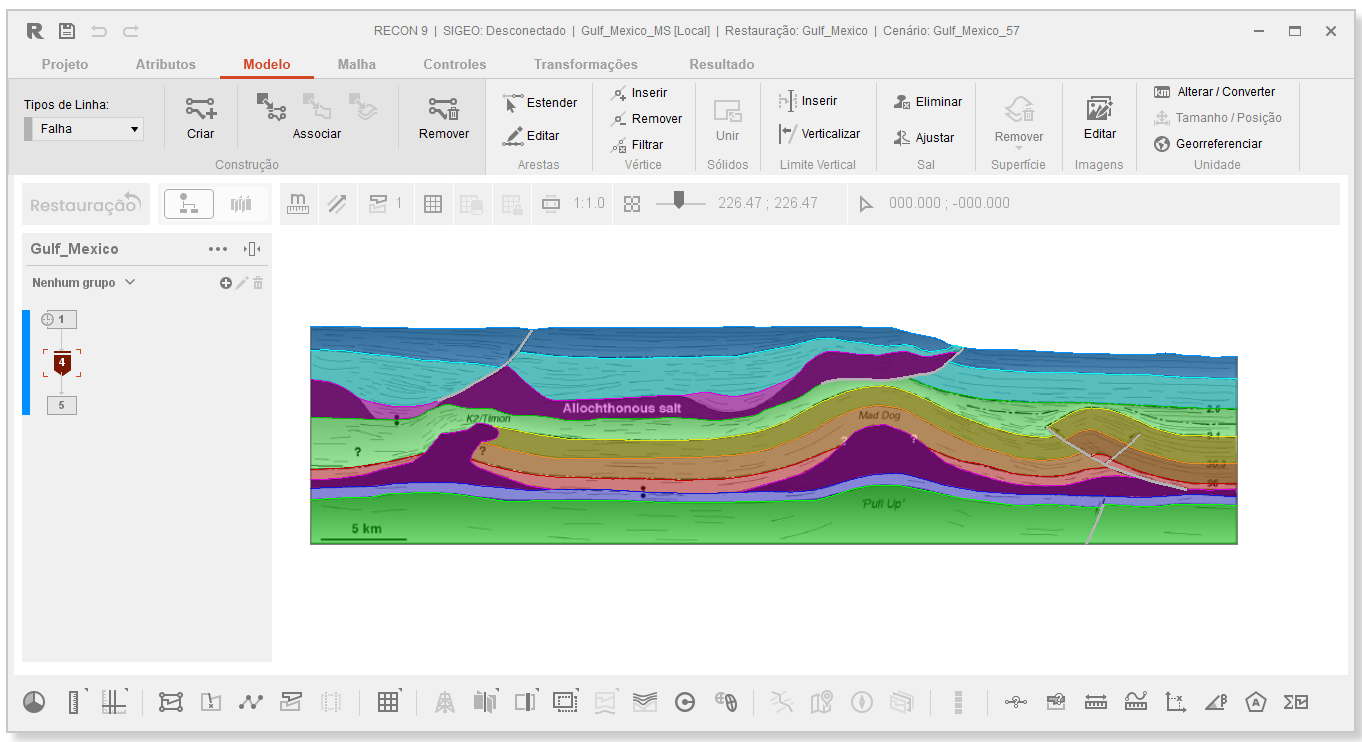
\includegraphics[width=\textwidth]{images/fig-recon}
    \caption{Captura de tela do Sistema Recon MS~\cite{Recon}.}\label{fig-recon}
  \end{center}
\end{figure}

De acordo com Fossen~\cite{Fossen}, restauração de seções geológicas pode ser entendida como uma manipulação da seção a fim de realizar a reconstituição dela ao seu estado anterior às deformações ocorridas ao longo do tempo. Em outras palavras, busca-se realizar uma retrodeformação na seção e utilizá-la na interpretação estrutural de uma região de interesse.

Um dos principais objetivos da restauração de uma seção geológica é a validação de sua interpretação estrutural. A validação se dá quando a retrodeformação identifica que o processo de formação da seção tem consistência geológica. Quando a restauração identifica essa consistência, a seção geológica é dita \emph{balanceada}. Por isso, o processo de restauração também é chamado de \emph{balanceamento} da seção geológica.

Neste capítulo são apresentadas as principais características do Sistema Recon MS para o objeto deste trabalho a fim de prover uma contextualização para o que é exibido nos demais capítulos. As próximas subseções tratam da descrição dos componentes principais e recursos básicos disponibilizados pelo sistema no processo de restauração de seções geológicas e também de visualização tridimensional do modelo. 

\subsection{Subdivisão Planar} % Falar do HED e da TopS

Segundo Berg~\cite{Berg}, uma subdivisão planar pode ser definida como uma subdivisão do plano através do uso de \textit{arestas}, \textit{vértices} e \textit{faces}. Essas são as entidades topológicas presentes em uma subdivisão planar, a face é uma região delimitada por arestas (segmentos de curva); os vértices são os limites das arestas, sendo um para cada extremidade (podendo ser o mesmo vértice no início e no final da aresta). Há ainda que se observar que a subdivisão planar é delimitada por uma face externa que representa o espaço no qual a subdivisão planar é definida.

A subdivisão planar precisa atender a alguns requisitos em relação às entidades topológicas: não deve haver vértices coincidentes; arestas só podem se cruzar em um vértice e faces também só se cruzam ou em um vértice, ou em uma aresta. Em outras palavras, não deve existir sobreposição de elementos topológicos. Uma ilustração na Figura~\ref{fig-subdivisao-planar-2} pode esclarecer como é a representação de uma subdivisão planar. Nessa imagem o plano é dividido em quatro regiões ($f_1$, $f_2$, $f_3$ e face externa) delimitadas por um conjunto de arestas.

\begin{figure} [h]
  \begin{center}
    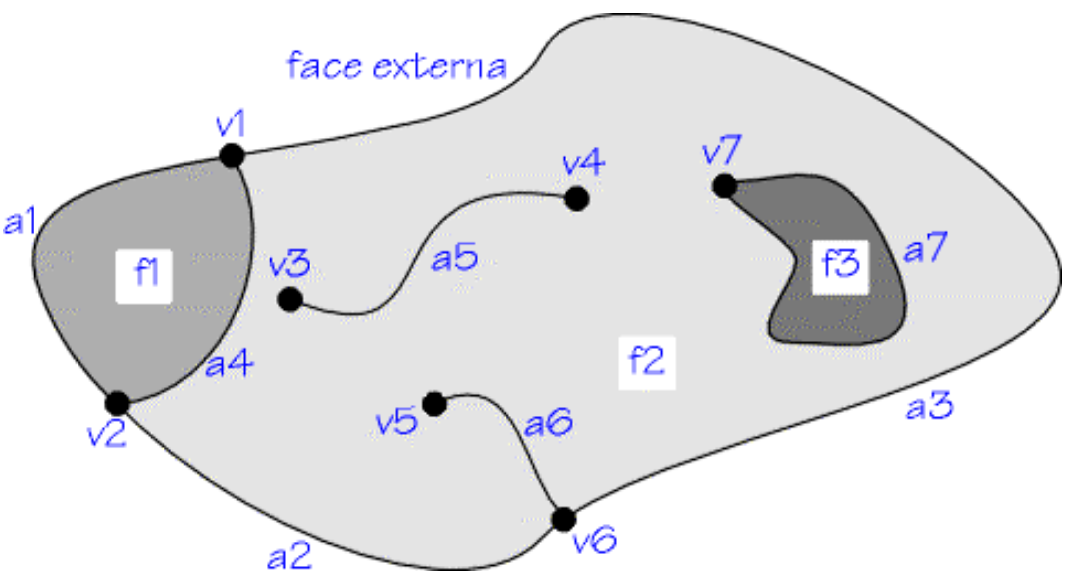
\includegraphics[width=\textwidth]{images/fig-subdivisao-planar-2}
    \caption{Representação de uma subdivisão planar~\cite{Ferraz}.}\label{fig-subdivisao-planar-2}
  \end{center}
\end{figure}

A nomenclatura dos componentes topológicos que formam a subdivisão planar são baseados na relação entre ela e sólidos homeomorfos a uma esfera. Uma vez que subdivisões planares são representações da topologia da fronteira desses sólidos~\cite{Cavalcanti}.

Em suma, a subdivisão planar tem os seguintes elementos topológicos~\footnote{Há ainda o elemento \emph{loop} ou laço que auxilia na definição de faces internas, porém para contextualização deste trabalho optou-se por apresentar apenas os elementos vértice, aresta e face.}:
\renewcommand{\labelitemi}{•}
\begin{itemize}
  \item \textbf{Vértice}: representa um ponto único dentro do plano.
  \item \textbf{Aresta} (edge): segmento de curva com vértices como limites.
  \item \textbf{Face}: região delimitada por um ou mais conjuntos conexos de arestas.
\end{itemize}

Uma seção geológica pode ser representada digitalmente por uma subdivisão planar uma vez que ela pode ser vista como um conjunto de polígonos que dividem o domínio da seção. Estes polígonos podem sofrer deformações e deslocamentos oriundos das transformações geológicas que a seção pode sofrer durante o balanceamento. Há ainda informações de adjacências entres essas porções que também precisam ser consideradas em um contexto computacional da seção geológica.

Na Figura~\ref{fig-subdivisao-planar} é possível perceber, por exemplo, que as camadas A, B e C possuem 3 blocos separados por falhas. Cada bloco é uma região fechada delimitada por um conjunto de segmentos. Deve-se observar ainda que essas regiões possuem atributos geológicos como idade, litologia, porosidade, etc. Mais informações a respeito dos atributos são apresentadas nas próximas subseções.

\begin{figure} [h]
  \begin{center}
    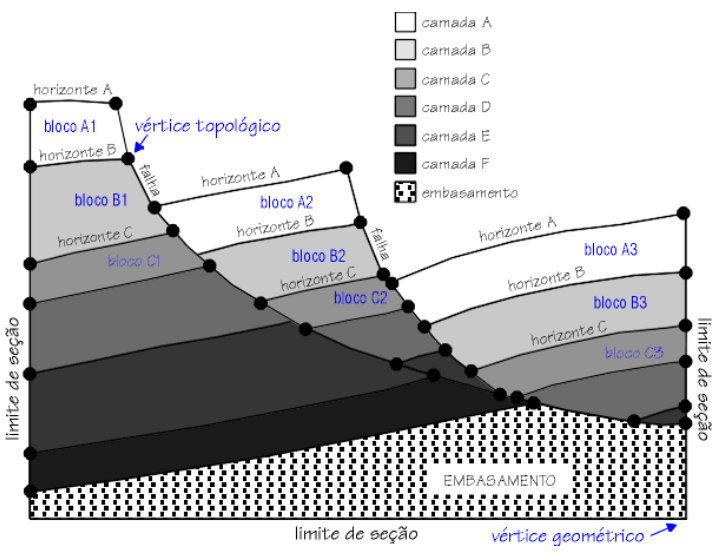
\includegraphics[width=\textwidth]{images/fig-subdivisao-planar}
    \caption{Seção geológica como uma subdivisão planar~\cite{Ferraz}}\label{fig-subdivisao-planar}
  \end{center}
\end{figure}

\subsection{Modelagem da Subdivisão Planar}

Para modelar a subdivisão planar dentro do Recon é utilizada a biblioteca computacional \emph{HED} (Half-EDge) desenvolvida pelo Instituto Tecgraf/PUC-Rio. Ela consiste na implementação de uma estrutura de dados topológicos baseada em arestas, a \textit{Half-Edge}~\cite{HED}, uma das razões para esta escolha são as relações fixas de adjacência que uma aresta apresenta em relação às outras componentes topológicas. Uma aresta sempre é delimitada por dois vértices (distintos ou não) e é adjacente à duas faces.

O HED introduz uma nova entidade que explora bem essa característica denominada \textit{half-edge} ou \textit{semiaresta} que é uma referência ao \quotes{uso} da aresta por uma face. Dessa forma, no HED, cada aresta é formada por duas semiarestas. Cada semiaresta guarda uma referência para uma face e também para um vértice de origem. Isto dá uma orientação para a semiaresta que é usada para indicar o sentido positivo da ordem dos vértices das faces, por exemplo.

A estrutura HED tem um aspecto hierárquico de listas duplamente encadeada de elementos topológicos. No nível mais alto está a subdivisão planar, denominada como \textit{HedSolid}, então vêm \textit{HedFace}, \textit{HedLoop}, \textit{HedHalfEdge} e \textit{HedVtx} no nível mais baixo. A representação da aresta, \textit{HedEdge} encontra-se no mesmo nível da \emph{HedHalfEdge}.

Uma propriedade importante em estruturas topológicas são as relações de adjacências entre suas componentes, a HED não provê de forma direta todas as relações, contudo é possível chegar às demais com uso de indireções. Por exemplo, partindo de uma aresta, como chegar às faces vizinhas? Basta ir às semiarestas da aresta, cada semiaresta possui referência para uma face.

Apresentado o HED e seus elementos, a associação com as entidades geológicas é intuitiva. Um bloco de camada geológica é representada por uma face; os segmentos de linhas de horizonte, falha ou borda de sal têm como correspondente as arestas, por último, cada conjunto contínuo de faces é associado a um sólido. Os sólidos representam uma subdivisão planar e, em alguns casos, a seção pode apresentar partes inteiramente descontínuas onde cada uma é um sólido diferente. Para casos onde é necessário sobreposição de partes, só é possível com a existência de mais de um sólido.

Destaca-se que a ideia de representar a seção geológica como uma subdivisão planar, ou uma estrutura HED, visa facilitar a criação e manipulação computacional da seção durante o processo de restauração. Todavia, a representação completa precisa levar em consideração também os atributos geológicos. Mais detalhes sobre a estrutura de dados HED podem ser encontrados em Mäntÿla~\cite{HED}, Arruda~\cite{Arruda} e Botsch \textit{et al.}~\cite{Botsch}.

\subsection{Atributos Geológicos}\label{geological-attributes}

Como dito, os blocos que formam a seção geológica possuem propriedades que também precisam estar salvas na estrutura de dados topológica.

Cada entidade do HED possui um campo reservado para um tipo genérico de informações. Nesse espaço reservado são organizados os atributos geológicos da seção e, portanto, o HED gerencia os atributos geológicos. Estes atributos são representados em estruturas chamadas \textit{GeoSolid}, \textit{GeoFace}, \textit{GeoEdge} e \textit{GeoVtx}. Pela nomenclatura, é fácil observar a relação com o HED. As principais informações organizadas nessas estruturas são:

\renewcommand{\labelitemi}{•}
\begin{itemize}
  \item \textbf{GeoSolid}: o sólido, por ser a estrutura de mais alto nível, guarda a referência à seção e ao cenário ao qual pertence dentro da restauração.
  \item \textbf{GeoFace}: é a estrutura que precisa armazenar dados do material geológico que a compõe (como idade, tipo, características físicas, etc.) e malha de triângulos que pode ser manipulada pelas transformações.
  \item \textbf{GeoEdge}: estrutura que guarda o tipo de linha (de horizonte, falha, topo de sal, etc.) e a subdivisão geométrica que forma a linha. 
  \item \textbf{GeoVtx}: é a única que armazena apenas o identificador universal.
\end{itemize}

Todas as estruturas de atributos geológicos possuem um campo para salvar este identificador que possui o formato \textit{UUID} --- \textit{universally unique identifier}~\cite{UUID} ou identificador único universal. Esse identificador é usado, por exemplo, na associação dos elementos geológicos com a malha triangular das faces, conforme é apresentado adiante.

\subsection{Seções Geológicas} % Falar da árvore de cenários

O Sistema Recon representa as seções geológicas pela estrutura descrita acima. Além disso, ele tem um conjunto de ferramentas para manipular uma seção geológica, desde a digitalização das informações que a definem geometricamente, da caracterização dos materiais e propriedades, da criação de dispositivos de controle e monitoramento da restauração, até o kit de transformações que irão deformar a seção.

\subsubsection{Criação de uma seção geológica}\label{item-section-creation}

Para criar uma seção geológica no Sistema Recon pode-se recorrer ao editor gráfico para desenhar linhas e atribuir propriedades manualmente conforme seu tipo (se for horizonte, falha, limites da seção, etc.). Alternativamente, em modelos que apresentem superfícies tridimensionais, como na Figura~\ref{fig-recon-1}, as seções podem ser criadas pela interseção de um plano vertical segundo uma direção dada pelo usuário. Essa ação é chamada de \textit{fatiamento} do modelo.

\begin{figure} [H]
  \begin{center}
    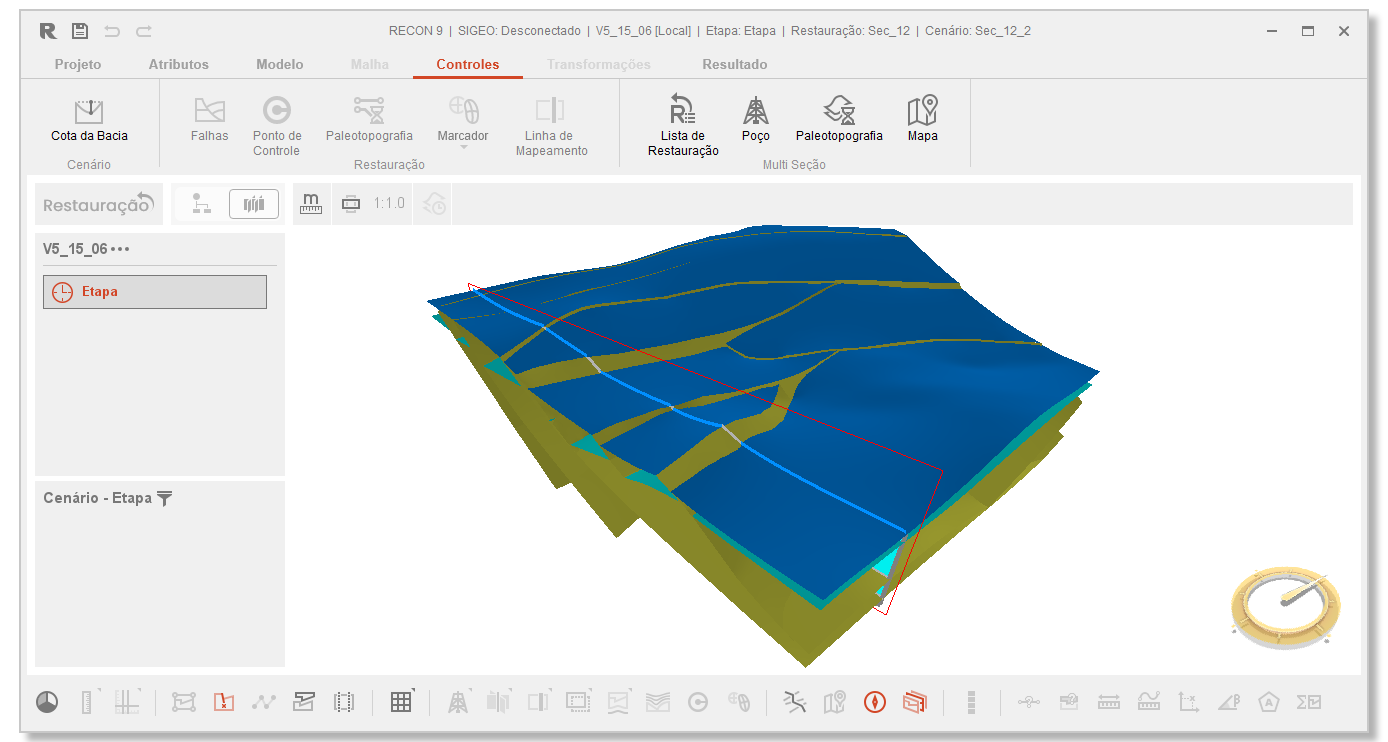
\includegraphics[width=\textwidth]{images/fig-recon-1}
    \caption{Sistema Recon exibindo um modelo com superfícies tridimensionais e uma seção em destaque.}\label{fig-recon-1}
  \end{center}
\end{figure}

\subsubsection{Malhas da seção geológica}

A seção geológica é representada como uma subdivisão planar, como já citado, e utiliza a biblioteca HED na representação dessa subdivisão. Na Figura~\ref{fig-recon-2} pode-se observar uma seção geológica e alguns elementos, como as linhas (\textit{HedEdges}) onde a sua cor representa o atributo de tipo e as faces (\textit{HedFaces}) que são, em termos simples, regiões fechadas por linhas. Neste exemplo, todas as faces pertencem à mesma camada geológica.

\begin{figure} [h]
  \begin{center}
    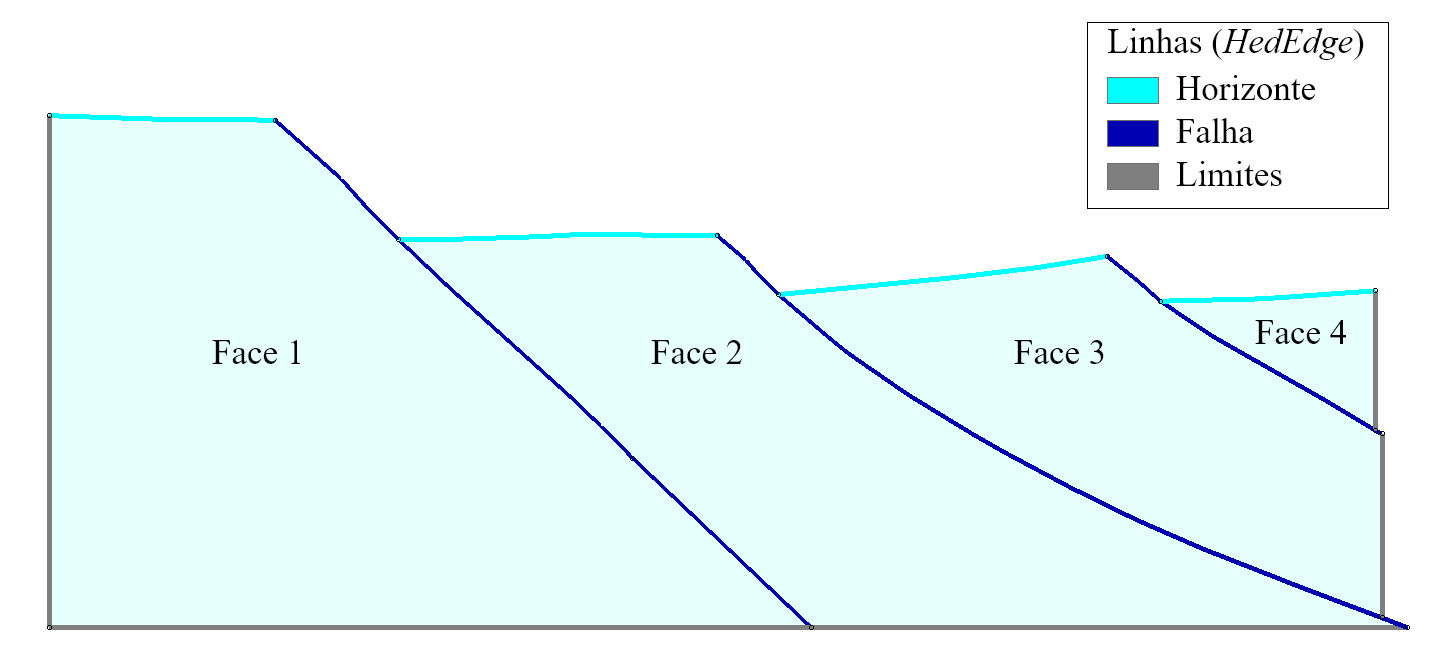
\includegraphics[width=\textwidth]{images/fig-recon-2}
    \caption{Seção geológica com destaque para os elementos de linhas e faces.}\label{fig-recon-2}
  \end{center}
\end{figure}

As faces têm um atributo muito importante para o trabalho de restauração, que são as malhas de triângulos. As malhas são penduradas por face para facilitar o uso, aproveitando-se do fato do HED gerenciar atributos. Neste caso, cada face possui uma malha independente das outras. 

No Sistema Recon, essa malha é armazenada numa estrutura de dados topológicos chamada \textit{TopS} (Topological Data Structure for Mesh Representation)~\cite{Tops} que trata-se de uma biblioteca computacional voltada para representação de malhas de elementos finitos. A Figura~\ref{fig-recon-3} exibe a mesma seção, mas com adição das malhas das faces.

\begin{figure} [H]
  \begin{center}
    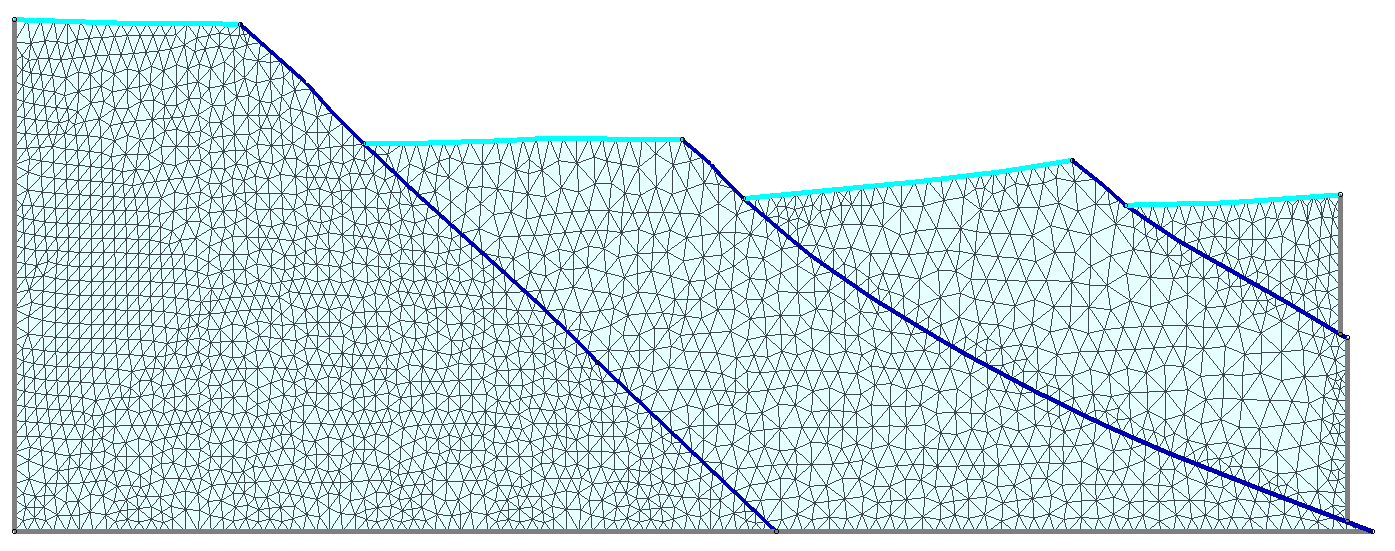
\includegraphics[width=350pt]{images/fig-recon-3}
    \caption{Malhas das faces de uma seção geológica no Sistema Recon.}\label{fig-recon-3}
  \end{center}
\end{figure}

A estrutura \emph{TopS}, assim como o HED, permite que sejam armazenadas informações em suas entidades topológicas. Em especial, nos vértices da malha, no Sistema Recon, é armazenado o \textit{UUID} do atributo geológico da entidade topológica do HED sobre a qual aquele vértice está localizado. Se o vértice da malha está no interior da face, ele guarda o \textit{UUID} da \textit{GeoFace} dessa face, o mesmo para caso esteja sobre uma aresta (\textit{GeoEdge}) ou vértice (\textit{GeoVertex}). A Figura~\ref{fig-recon-4} mostra um exemplo da forma como esses dados são obtidos.

\begin{figure} [H]
  \begin{center}
    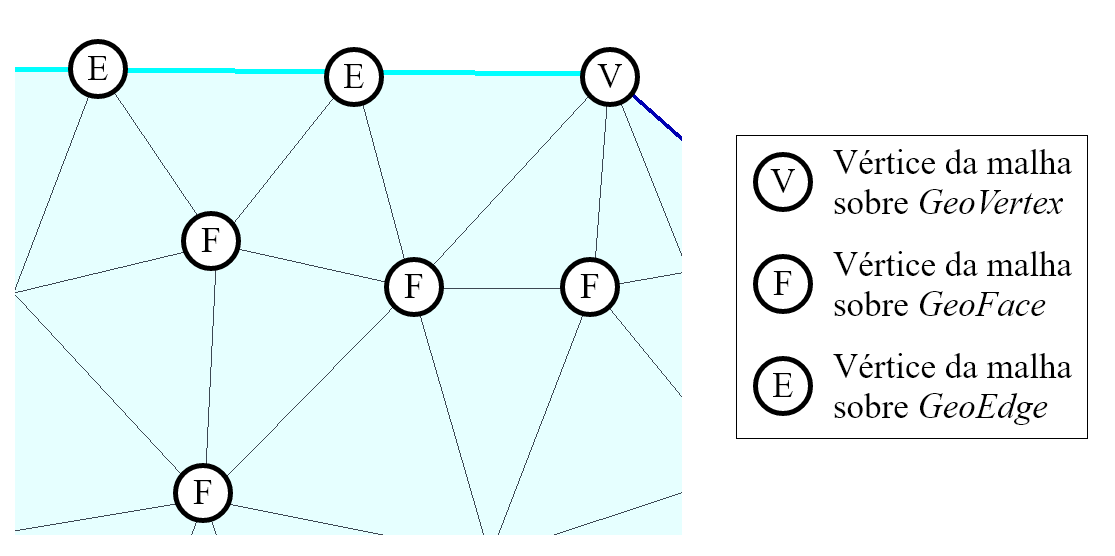
\includegraphics[width=\textwidth]{images/fig-recon-4}
    \caption{Trecho de uma malha de face com os tipos de atributo geológicos que estão sob os vértices da malha.}\label{fig-recon-4}
  \end{center}
\end{figure}

Essa relação permite identificar, a partir de um vértice da malha, sobre qual entidade geológica está este vértice. O uso desse recurso é descrito no próximo capítulo.

Salienta-se que a adoção da \emph{TopS} para gerenciar a malha da faces se dá pelos recursos que essa estrutura fornece para a representação de malhas, como pode ser consultado em Celes \emph{et al.}~\cite{Tops}. As malhas, no Sistema Recon, são atributos das faces e são armazenadas na estrutura \emph{GeoFace} contida no HED, como explicado no item~\ref{geological-attributes}.

As malhas de faces dentro do Sistema Recon, além de serem utilizadas como marcadores de deformações provocados por transformações geológicas ao longo da restauração de uma seção, tem também um uso relacionado ao mapeamento de informações nessa seção. As malhas permitem ter um acompanhamento geométrico de objetos como pontos e linhas no decorrer do processo de restauração. Há ainda a possibilidade de, a partir da deformação da malha, realizar uma deformação na imagem usada para digitalização da seção.

\subsubsection{Transformações geológicas}

As transformações geológicas são procedimentos que buscam reverter (ou simular) as movimentações e deformações ocorridas ao longo do tempo~\cite{Santi}. As transformações são aplicadas às entidades topológicas de uma seção geológica e também são aplicadas às malhas das faces. No entanto, para que isso aconteça, é necessário antes a definição de \textit{Módulos} na seção. 

Módulos são agrupamentos de faces ou blocos da seção submetidos a uma mesma movimentação ou efeito tectônico. Isso é um recurso importante para estabelecer relação entre a modelagem geométrica e a Geologia. No Sistema Recon, módulos são criados e destruídos dinamicamente para se aplicar as transformações geológicas desejadas.

Com o módulo definido, consegue-se aplicar uma transformação. Esta irá ser aplicada à malha de cada uma das faces que compõem aquele módulo.

Como visto na Figura~\ref{fig-recon-5} as transformações geológicas se dividem em grupos conforme o tipo de regime tectônico. Para os modelos aos quais este trabalho se propõe, podem se destacar as transformações do grupo \emph{Distensivo} e também as \emph{Gravitacionais} como a descompactação que trata da remoção da camada do topo, geralmente após a restauração desta, o que acaba por gerar um aumento na espessura das camadas inferiores. Mais informações sobre as transformações presentes no Sistema Recon MS podem ser consultadas no manual do usuário do sistema~\cite{Recon}.

\begin{figure} [H]
  \begin{center}
    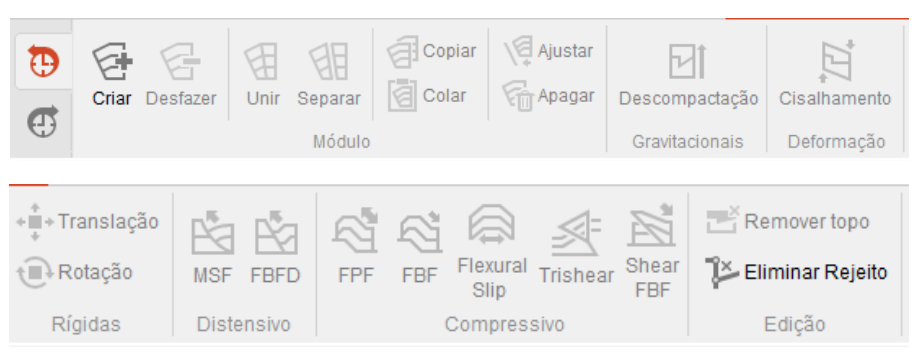
\includegraphics[width=\textwidth]{images/fig-recon-5}
    \caption{Aba \quotes{Transformações} do Sistema Recon.}\label{fig-recon-5}
  \end{center}
\end{figure}

\subsubsection{Árvore de cenários}

A restauração de seções é um processo linear no sentido de que cada novo passo depende do estado no passo anterior. Qualquer decisão sobre uma transformação geológica em um passo desses acarreta em um resultado diferente ao final. Além do mais, balanceamento de seções não é uma atividade de resposta única, o objetivo é obter uma interpretação geológica plausível para a seção geológica atual, ou seja, uma interpretação que permita que seus componentes estruturais possam ser restaurados~\cite{Fossen}. 

Diante disso, o Sistema Recon disponibiliza em sua interface de manipulação das seções um componente capaz de registrar o histórico de etapas no processo de restauração. Mais que isso, ao usuário é dada a possibilidade de voltar em algum ponto e criar uma nova linha de estudo dentro desse processo, ou ainda apagar uma sequência de etapas que ele julga estar incorreta.

Isso tudo é possível graças a uma estrutura de dados representada graficamente através de um componente de interface que auxilia na tomada de decisões no processo de tentativa e erro. Essa estrutura de dados é chamada árvore de cenários. Um cenário é a representação de um estado de restauração de uma seção. Por exemplo, se de um passo a outro da restauração ocorre uma transformação, o estado anterior pode ser registrado em um cenário e o posterior em um outro. De cada cenário pode-se criar diversos outros como se fossem diferentes linhas do tempo, ou diferentes interpretações daquele passo de restauração.

Árvores são um tipo especial de estrutura de dados e neste caso de uso é definida como tendo uma raiz ou nó inicial que aponta para um ou mais nós. Estes, igualmente, podem apontar para diferentes nós numa escala hierárquica. A Figura~\ref{fig-recon-6} apresenta um exemplo de árvore de cenários tirada do Sistema Recon. Nesta imagem, cada quadrinho representa a seção num dado estado e como identificação, cada cenário também possui um número.

\begin{figure} [H]
  \begin{center}
    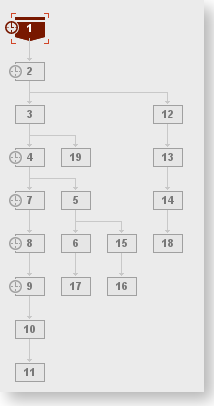
\includegraphics[width=160pt]{images/fig-recon-6}
    \caption{Exemplo de árvore de cenários de uma seção do Sistema Recon.}\label{fig-recon-6}
  \end{center}
\end{figure}

Um requisito para que se faça a restauração da seção é a definição do chamado \emph{cenário origem}, que é aquele que representa a seção em sua configuração original. Na Figura~\ref{fig-recon-6} o cenário origem é o número 1 e pode ser visto com uma representação especial na árvore de cenários. Um cenário, para ser marcado como \emph{origem}, precisa ter todas as malhas já definidas incluindo outras condições. Além disso, após a marcação como origem, esse cenário não pode ser modificado e dessa forma pode ser usado como uma referência para outros processos dentro do Sistema Recon.

A cada nova manipulação da seção pode-se criar um novo cenário e assim ter este histórico da restauração. Essa maneira de organizar uma restauração é útil não só no contexto de uma seção isolada, mas principalmente quando se trabalha em modelos de multisseções que irão sofrer os mesmos processos de restauração, mas de maneiras diferentes. Com um registro do quê e quando ocorreu uma dada transformação em diferentes seções é possível ter uma visão mais geral do modelo em uma sequência cronológica.

\subsection{Ambiente Multisseções}

Apesar dos principais recursos do Sistema Recon atuarem diretamente com seção geológica, isso não significa dizer que só seja possível manipular modelos com uma única seção geológica. Uma das grandes mudanças ocorridas no programa ao longo dos anos foi a criação de ferramentas para tratar de modelos com múltiplas seções, ou modelos multisseção~\cite{Felipe, Garcia}. A versão usada neste trabalho traz um importante recurso para a manipulação desses modelos: o ambiente multisseção.

O ambiente multisseção (MS) do Sistema Recon trata-se de um visualizador 3D onde podem ser vistas as superfícies geológicas e também as seções em um contexto global do modelo.

Como sistema de referências, o ambiente MS usa coordenadas UTM (Universal Transversa de Mercador)~\cite{IBGE} para localizar seus objetos. Neste sistema, cada ponto é representado por um par $(N, E)$ onde $N$ é a coordenada norte-sul em metros e $E$, a coordenada leste-oeste.

A Figura~\ref{fig-recon-7} exibe o Sistema Recon no ambiente MS, onde é possível notar o (1) visualizador tridimensional com superfícies e seções geológicas, (2) a lista de \textit{EtapasMS} que será apresentada a seguir juntamente da (3) lista de cenários da etapa.

\begin{figure} [H]
  \begin{center}
    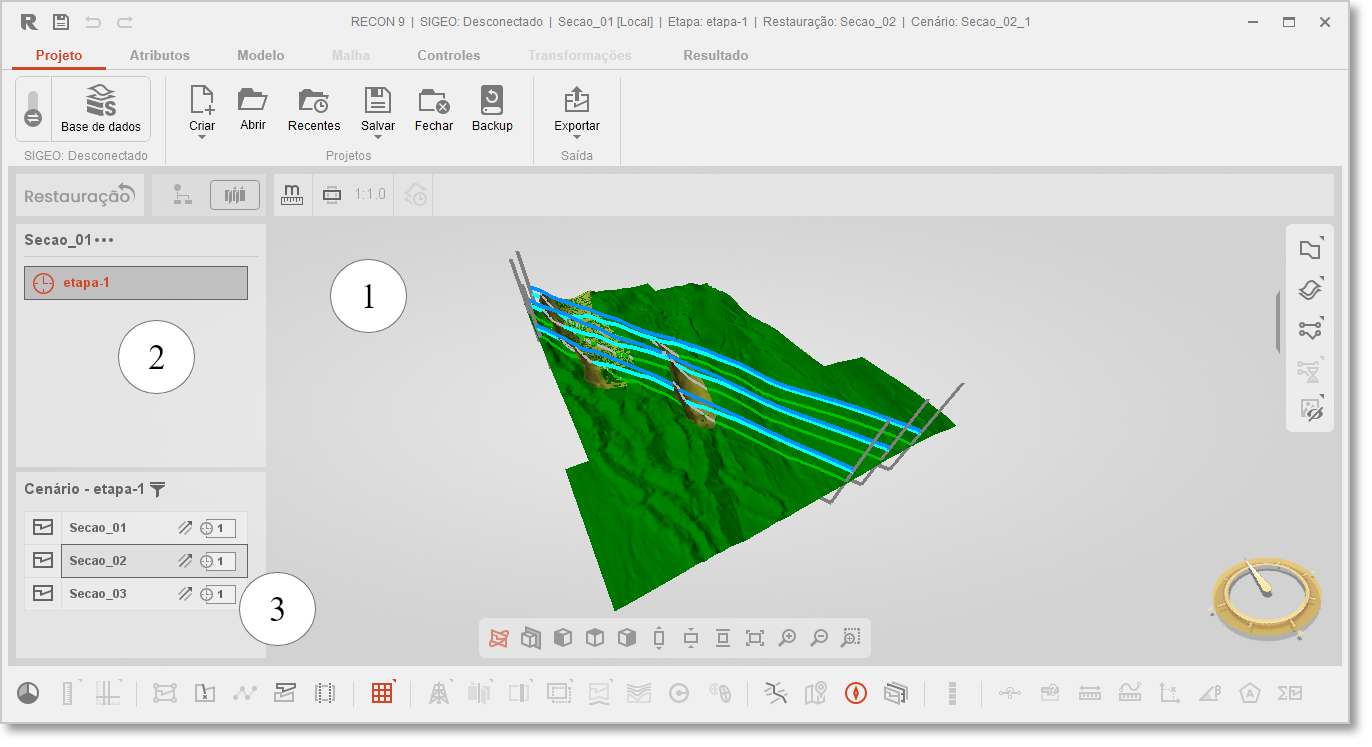
\includegraphics[width=\textwidth]{images/fig-recon-7}
    \caption{Ambiente Multisseção do Sistema Recon.}\label{fig-recon-7}
  \end{center}
\end{figure}

\subsection{Etapas de restauração}\label{step-ms}

Como brevemente apresentado, o ambiente MS permite ter um olhar mais global do modelo e de todos os componentes que o formam. Nesse contexto é então preciso organizar as seções de forma que haja o máximo de coerência do ponto de vista geral durante a restauração do modelo. Podem existir seções que compartilham uma mesma falha ou um mesmo evento tectônico, por exemplo.

Como já visto, cada seção conta com um registro de cada passo dado no andamento da restauração e é um recurso presente apenas localmente e independente. No entanto, seções relativamente próximas, ou que foram restauradas de maneira semelhante precisam sincronizar esse histórico para que haja uma ordem melhor do modelo sob um aspecto global.

Com essa finalidade, esta versão do Sistema Recon também possui o conceito e implementação da \textit{EtapaMS}. Uma \textit{EtapaMS} trata-se de um conjunto de cenários de seções diferentes mas que, de certa forma, representam o mesmo marco geológico, como a restauração de uma falha ou descompactação. Cada \textit{EtapaMS} pode ter apenas 1 cenário por seção dentro de sua estrutura, isso permite ter um histórico do modelo multisseção análogo à árvore de cenário da seção individualmente.

No Sistema Recon, as \textit{EtapasMS} são dispostas em lista no ambiente multisseção. Ao selecionar um item dessa lista, logo abaixo é exibido o conjunto de cenários (por seção) que compõem aquela \textit{EtapaMS}, como mostra a Figura~\ref{fig-recon-7}.

Uma forma de uso das \textit{EtapasMS} para a restauração de modelos geológicos é organizar os estados de seções diferentes que respondam ao mesmo evento ou marco geológico. Caso haja uma falha X que atravessa 3 seções e em todas elas essa falha é restaurada, pega-se o cenário de cada seção onde isso ocorre e cria-se uma \textit{EtapaMS} correspondente a este marco. As \emph{EtapasMS} permitem que haja um sincronismo entre as seções onde ocorreram um mesmo evento geológico. Esta organização da restauração é parte muito importante para o mapeamento de superfícies e volume.



  % -*- coding: utf-8; -*-

\chapter{Linhas de Mapeamento}

O mapeamento descrito neste trabalho é baseado exclusivamente na restauração de seções geológicas. Para tanto, há a necessidade de uma camada de informações proveniente das seções que contenha os dados a serem usados no mapeamento tridimensional. Essas informações podem ser extraídas com auxílio de um objeto geométrico auxiliar presente nas seções geológicas: \textit{linhas de mapeamento}.

Neste capítulo é apresentado o conceito de linha de mapeamento existente no Sistema Recon, suas características, alguns casos de uso e também suas derivações.

\section{Conceito}

Linhas de mapeamento são linhas formadas por \textit{pontos de mapeamento}. Estes pontos são objetos mapeados nas malhas da seção e guardam a informação referente à sua localização dentro desta malha.

Um ponto de mapeamento, em razão dos tipos de entidades topológicas presentes na malha, pode ser do tipo nó, aresta ou elemento:

\renewcommand{\labelitemi}{•}
\begin{itemize}
  \item Nó: o ponto está sobre um nó da malha. É guardado o identificador desse nó.
  \item Aresta: caso onde o ponto localiza-se sobre uma aresta de elemento. Além do identificador da aresta, é armazenada a coordenada paramétrica do ponto na aresta.
  \item Elemento: o ponto encontra-se no interior de um elemento. Guarda-se o identificador do elemento e as coordenadas baricêntricas do ponto no elemento triangular.
\end{itemize}

A criação dessas linhas se dá pela definição de uma linha-guia que pode cruzar diferentes regiões da seção. Para cada região interceptada, é criada uma parte de linha de mapeamento, essa parte armazena o identificador da malha da região. A interseção dos pontos da linha-guia com a malha produz os pontos de mapeamento.

A linha de mapeamento pode ser criada em qualquer cenário durante a restauração da seção e sua geometria pode ser calculada com base na malha em função dos pontos de mapeamento que a formam. Após a criação, uma versão da linha de mapeamento é gerada para cada cenário anterior e subsequente ao que foi usado na definição da linha-guia. Com isso, pode ser realizado o mapeamento dessa linha ao longo das etapas de restauração da seção.

O requisito para que seja calculada a geometria da linha em diferentes cenários é que a malha mantenha a mesma topologia. No entanto, mesmo em casos de edição, é possível realizar uma interpolação dos atributos presentes na malha para sua nova versão. Incluem-se nisso as partes de linha de mapeamento que irão também receber uma nova versão equivalente dada a alteração na topologia da malha.

Dentro do Sistema Recon MS, a linha de mapeamento é um recurso importante na interpretação dos resultados gerados na restauração do modelo. Com ela é possível ter uma linha que acompanha a movimentação da malha de um cenário a outro.

As linhas de mapeamento (Figura~\ref{fig-linemap}) permitem realizar um mapeamento geométrico ao longo de uma restauração tomando como base uma linha-guia poligonal definida pelo usuário.

\begin{figure} [h]
  \begin{center}
    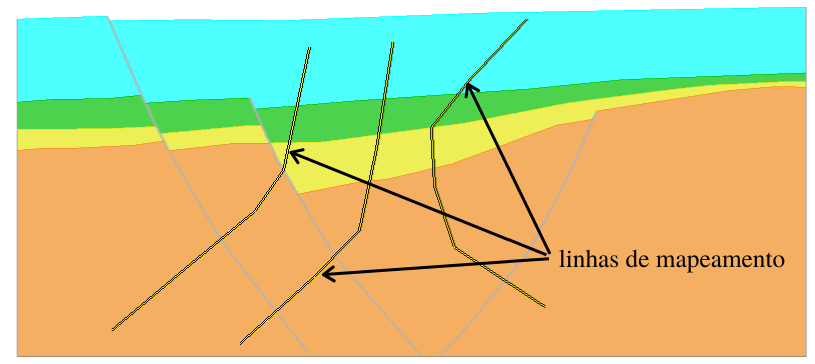
\includegraphics[width=\textwidth]{images/fig-linhas-de-mapeamento-ed}
    \caption{Linhas de mapeamento em uma seção.}\label{fig-linemap}
  \end{center}
\end{figure}

A Figura~\ref{fig-linemap-history} apresenta o resultado após uma transformação do tipo \textit{move sobre falha} (MSF)~\cite{Recon} onde é possível observar, além da deformação da camada, a linha de mapeamento sofrendo a mesma movimentação. Este tipo de uso pode ser interpretado como se houvesse ali um falso horizonte para avaliar o quantidade de movimento na restauração do rejeito.

\begin{figure} [h]
  \begin{center}
    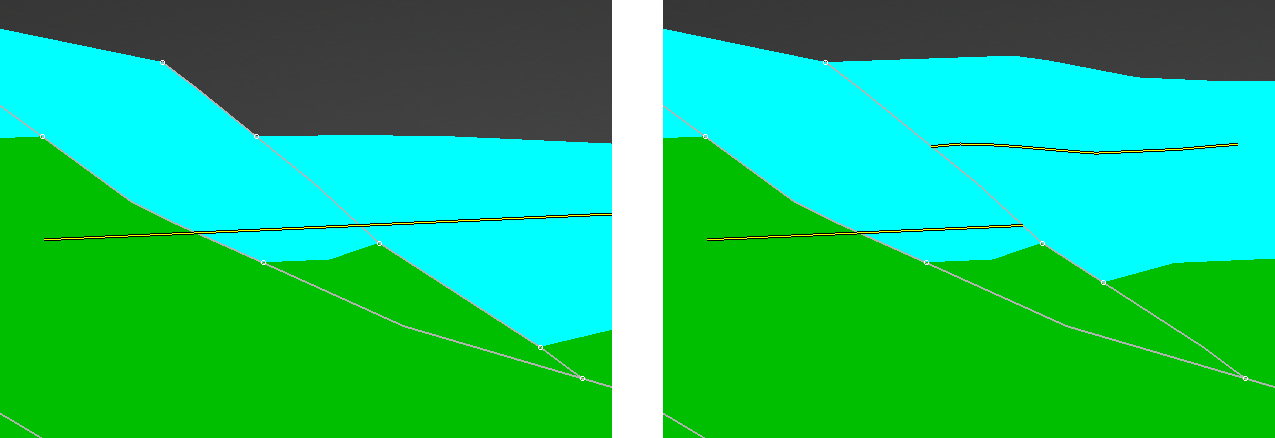
\includegraphics[width=\textwidth]{images/fig-linemap-history}
    \caption{Linhas de mapeamento em diferentes etapas}\label{fig-linemap-history}
  \end{center}
\end{figure}

\section{Criação das Linhas de Mapeamento}

O processo de criação da linha de mapeamento é feito para cada parte individualmente, de forma que, ao visualizar as partes tem-se a linha de mapeamento completa. Na Figura~\ref{fig-linemap-malhas} é possível ver uma linha de mapeamento cortando algumas regiões diferentes.

\begin{figure} [h]
  \begin{center}
    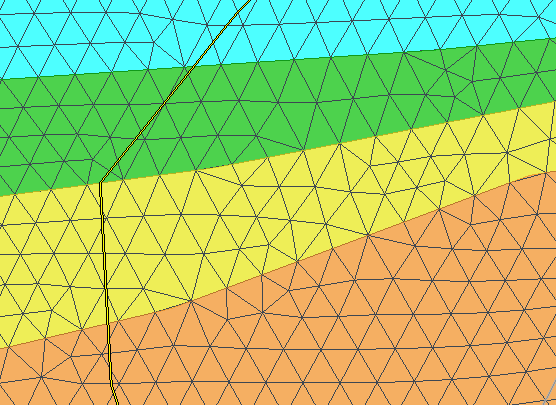
\includegraphics[width=250pt]{images/fig-linhas-de-mapeamento-malhas}
    \caption{Linhas de mapeamento cortando múltiplas faces.}\label{fig-linemap-malhas}
  \end{center}
\end{figure}

Na Figura~\ref{fig-linemap-parts} estão evidenciadas as partes que formam a linha de mapeamento. Como já dito, cada parte está associada à malha de um região diferente.

\begin{figure} [h]
  \begin{center}
    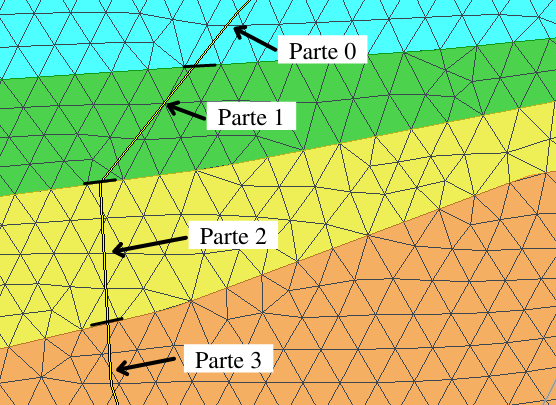
\includegraphics[width=250pt]{images/fig-lm-parts}
    \caption{Partes de uma linha de mapeamento}\label{fig-linemap-parts}
  \end{center}
\end{figure}

A Figura~\ref{fig-lm-topo} mostra a identificação dos pontos em uma parte de linha de mapeamento e a Tabela~\ref{tab-lm-topo} exibe quais informações topológicas são salvas de cada ponto.

\begin{figure} [hbt!]
  \begin{center}
    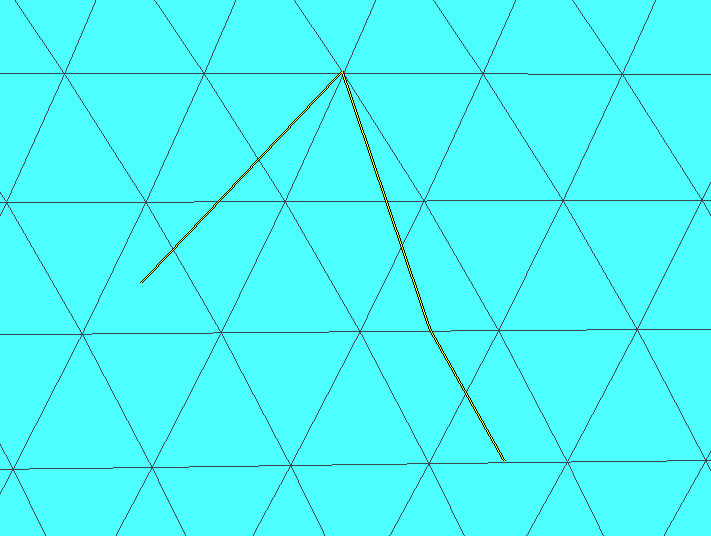
\includegraphics[width=260pt]{images/fig-lm-topo}
    \caption{Informações topológicas da malha mapeadas para a linha de mapeamento.}\label{fig-lm-topo}
  \end{center}
\end{figure}

% -*- coding: utf-8; -*-

\begin{table} [hbt!]
 \begin{center}
	 \caption{Informações topológicas salvas na linha de mapeamento.\label{tab-lm-topo}}
	~\\[-2mm]
	 \begin{tabularx}
		 {\textwidth}
		 {cp{2.0cm} lp{3.0cm} lp{10.0cm}}

		 \textbf{Ponto}
		 & \textbf{Tipo}
		 & \textbf{Informação armazenada} \\ \toprule

		 %~\\[-1mm]
		 A
		 & Elemento
		 & id=30, coordenadas baricêntricas=(0,33; 0,33; 0,33) \\ \midrule

		 %~\\[-1mm]
		 B
		 & Nó   
		 & id=431 \\ \midrule

		 %~\\[-1mm]
		 C
		 & Aresta
		 & id=130, coordenada paramétrica=0,45 \\ \midrule

		 %~\\[-1mm]
		 D
		 & Aresta
		 & id=145, coordenada paramétrica=0,55 \\ \midrule

	 \end{tabularx}
 \end{center}
\end{table}


\section{Derivações das Linhas de Mapeamento}

As linhas de mapeamento têm também casos de usos mais especializados dentro do Sistema Recon, como na criação e representação de poços. Poços são criados semelhantemente às linhas ou por importação de modelos com poços em 3D. Possuem característica de seguir a trajetória do poço e possuem uma finalidade mais limitada. Nos casos de poços 3D, a linha correspondente ao poço é apenas uma projeção do objeto tridimensional no plano da seção.

Há o uso nas chamadas linhas de interseção (\textit{CrossLine}) que servem para identificar e mapear as linhas de cruzamento entre seções no espaço tridimensional do multisseções, com isso é possível ter uma noção do que ocorre com seções transversais mesmo estando no domínio bidimensional da restauração.

Por último, foi criada a \textit{linha de mapeamento do modelo} ou \textit{LMModel}, cujo objetivo é servir para o mapeamento de linhas geológicas das seções para superfícies de horizontes geológicos e falhas. As \emph{LMModels} representam os elementos geológicos ao longo da restauração do modelo. Assim, é possível ter um acompanhamento do que ocorre com as entidades geológicas na seção, além de poder verificar como se deu a movimentação de cada ponto de horizonte, falha ou topo de sal ao longo da restauração.

As \textit{LMModels} são linhas de mapeamento baseadas no pontos do contorno da malha das regiões, ou seja, as partes que a formam possuem apenas pontos de mapeamento do tipo nó.

Pelo objetivo proposto, as \textit{LMModels} são linhas de mapeamento que tomam a geometria das entidades geológicas como entrada. Então, não há necessidade de criar uma linha-guia como é feita na linha de mapeamento original; a própria linha de horizonte, falha, ou topo de sal é usada como linha-guia.

Conforme o tipo do elemento geológico base, há um tipo de \textit{LMModel} e informações adicionais armazenadas:

\renewcommand{\labelitemi}{•}
\begin{itemize}
  \item Horizonte: a informação de idade deste horizonte.
  \item Falha: o identificador da falha é o dado armazenado.
  \item Topo de sal: apenas uma referência direta à linha original.
\end{itemize}

Todas essas informações  geológicas atreladas ao mapeamento topológico das \textit{LMModels}, quando em conjunto com as diversas seções geológicas de um modelo multisseções, são o que fazem dela o principal dado para a realização de um mapeamento de informações de evolução do modelo tridimensional ao longo do tempo, já que trazem todo o histórico de movimentação das camadas de um modelo geológico.

A utilização das \emph{LMModels} neste trabalho é feito com o auxílio de estruturas de dados que organizam as informações em subconjuntos divididos por etapa de restauração e idade (caso de linhas de horizonte), o que é visto na sequência. Com isso, é obtido o conjunto de informações que representam a restauração das seções no Sistema Recon.

\begin{figure} [h]
  \begin{center}
    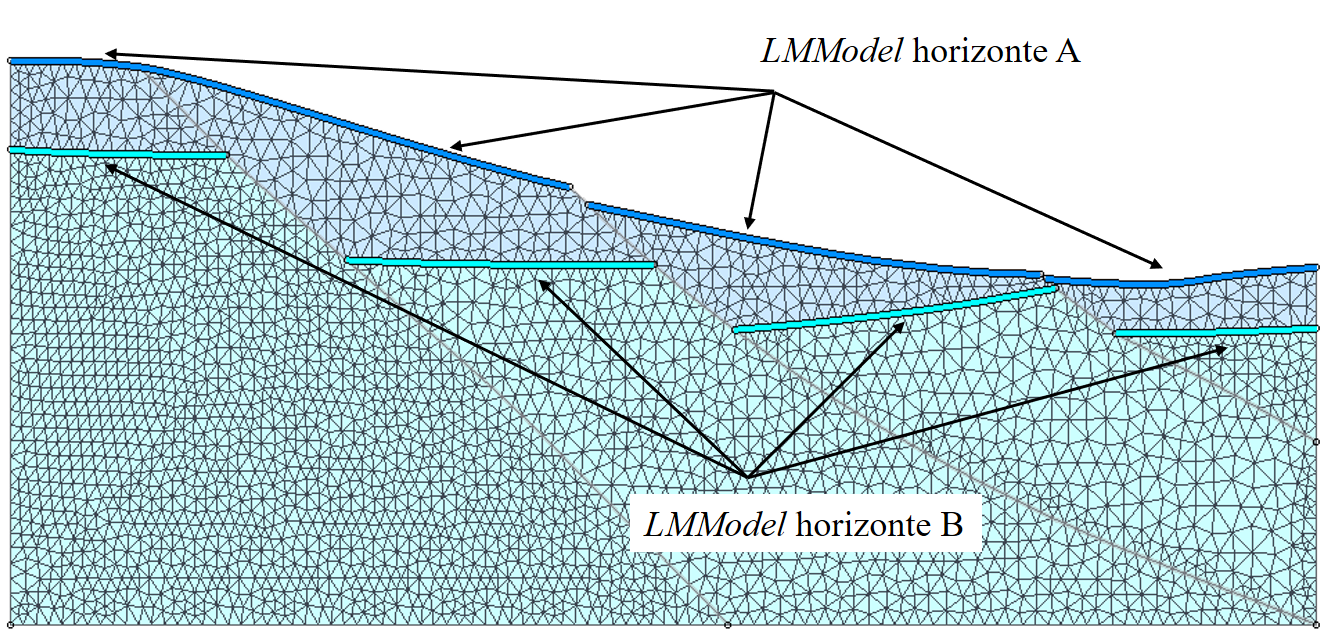
\includegraphics[width=350pt]{images/fig-lmmodel-example}
    \caption{\textit{LMModels} em uma seção geológica no Sistema Recon}\label{fig-lmmodel-example}
  \end{center}
\end{figure}

A Figura~\ref{fig-lmmodel-example} mostra \textit{LMModels} de dois horizontes diferentes. A representação delas dentro do Sistema Recon é feita com uma linha de maior espessura que as linhas de horizonte. No entanto, os pontos são os mesmos do contorno da malha. Observa-se na Figura~\ref{fig-lmmodel-mesh-diff} a diferença entre a linha de horizonte e a \textit{LMModel}, evidenciando o contorno da malha entre as duas regiões.

\begin{figure} [h!]
  \begin{center}
    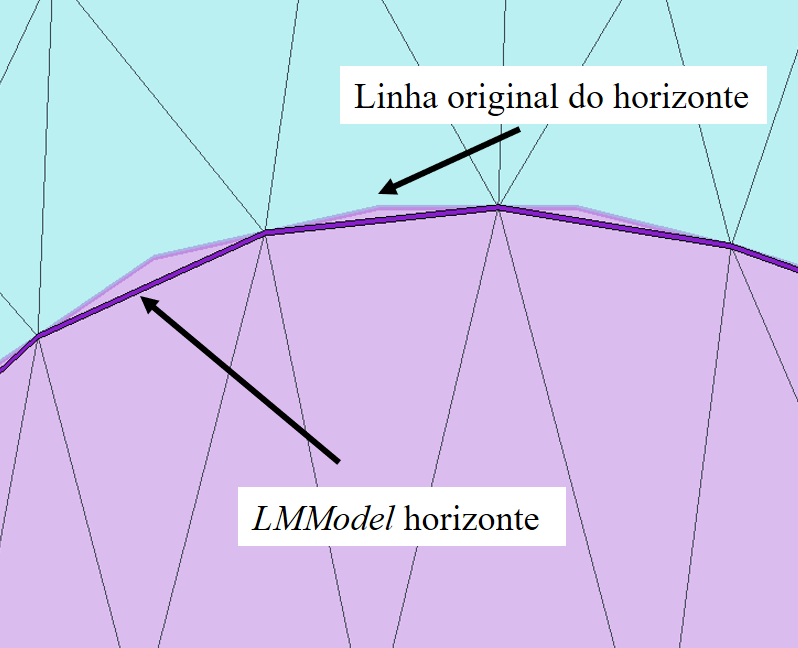
\includegraphics[width=275pt]{images/fig-lmmodel-mesh-diff}
    \caption{Diferença entre \textit{LMModel} e a linha de horizonte e uma seção geológica no Sistema Recon}\label{fig-lmmodel-mesh-diff}
  \end{center}
\end{figure}

A ilustração na Figura~\ref{fig-lmmodel-ms} apresenta as \textit{LMModels} de dois horizontes em um modelo multisseções. É esse conjunto de informações no ambiente tridimensional que será usado como parâmetro para o mapeamento de superfícies no Sistema Recon.

\begin{figure} [h!]
  \begin{center}
    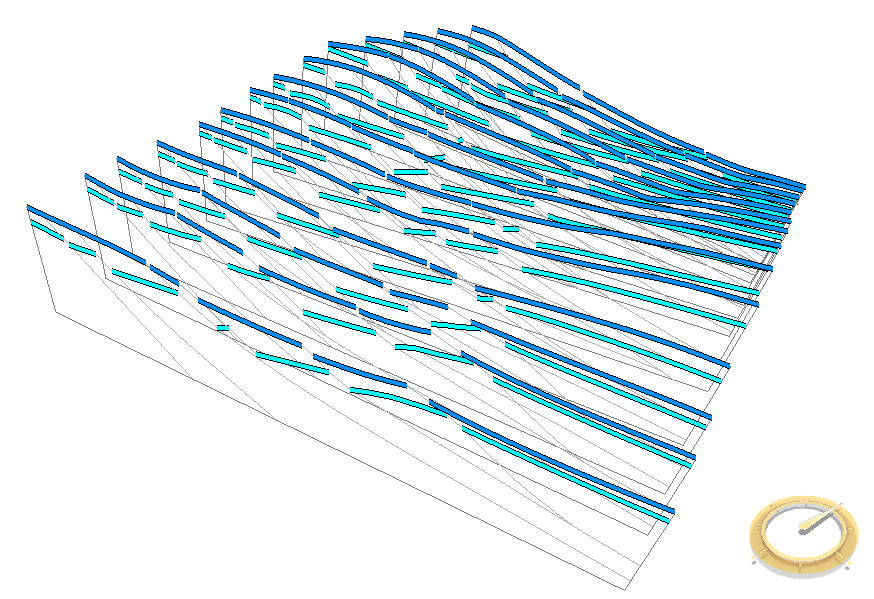
\includegraphics[width=300pt]{images/fig-lmmodel-ms}
    \caption{\textit{LMModels} no ambiente multisseções do Sistema Recon}\label{fig-lmmodel-ms}
  \end{center}
\end{figure}

A partir das \emph{LMModels} é possível obter o histórico de deslocamentos das linhas de horizontes ao longo do processo de restauração. As \emph{LMModels} são usadas no processo de mapeamento de superfícies como \emph{pontos de controle} para o deformador de superfícies que é apresentado no capítulo seguinte.



  % -*- coding: utf-8; -*-

\chapter{Mapeamento de superfícies}

No capítulo anterior foi apresentada a criação de linhas de mapeamento nas seções geológicas que servem como pontos de controle para o mapeamento das deformações sofridas pelas diversas seções para deformações das superfícies na restauração geológica tridimensional no Sistema Recon. Este capítulo mostra o mapeamento de superfícies que, neste trabalho, pode ser definido como o uso de informações das seções geológicas como parâmetros matemáticos para deformar os pontos da superfície e assim obter uma configuração coerente com a movimentação tectônica resultante da restauração das seções geológicas. A metodologia descrita a seguir foi apresentada por Müller~\cite{Muller} para tratar a deformação de superfícies com o uso de restrições presentes no domínio da mesma e através de minimização de uma energia.

\section{Metodologia}\label{surface-mapping-metodology}

A deformação de uma superfície pode ser modelada como um problema variacional com funções Lagrangeanas descritas pelo operador de Laplace com diferentes ordens e que podem descrever diferentes energias. A energia de superfície de membrana é uma EDP (equação diferencial parcial) de segunda ordem, descrita pelo operador de Laplace $\Delta{q}$ e a equação $\Delta{q}=0$ minimiza a área da superfície. A energia de placas-finas que minimiza a curvatura da superfície é descrita pela EDP de quarta ordem $\Delta^2{q}=0$. Já para minimização da variação da curvatura de superfícies pode ser usada uma EDP de sexta ordem, ou tri-harmônica, $\Delta^3{q}=0$, e a superfície resultante desta minimização é dita superfície de mínima variação~\cite{Muller, Botsch}.

A deformação de uma superfície pode ocorrer com base em duas premissas: que sejam conhecidas a posição inicial dos pontos da superfície e a posição deformada de pontos de controle (que também pertencem à superfície). A partir da informação desses pontos de controle busca-se encontrar a posição deformada de todos os pontos da superfície. A solução desse problema começa na obtenção de uma solução estacionária que minimize uma energia~\cite{Muller}.

Dois tipo de métodos podem ser usados para, dada uma superfície $\mathcal{S}$ num espaço $R^3$ com contorno $\Omega$ descrita num espaço cartesiano $x$ com pontos iniciais conhecidos e pontos de controle cujas deformações são conhecidas, calcular a deformação de $\mathcal{S}$. Os métodos baseados em superfície que dependem de uma boa qualidade da representação discreta da superfície e os baseados em deformação espacial que, como diz o nome, não dependem da representação da superfície~\cite{Botsch}. Dentre este últimos, cita-se: 

\renewcommand{\labelitemi}{•}
\begin{itemize}
  \item o método Lattice Based Freeform Deformation, usa funções de forma B-spline e um tensor descrito pelos pontos de controle, sua formulação resulta em um sistema retangular de equações lineares solucionável por meio de inversas generalizadas ou mínimos quadrados;
  \item o método Cage Based Freeform Deformation, pode ser considerado uma generalização do método anterior e utiliza uma gaiola de malha grossa que engloba a superfície a ser deformada e uma interpolação linear entre os pontos da gaiola e os pontos de controle que por sua vez compõem novas funções de interpolação;
  \item o método com Radial Basis Functions (RBF), conhecido por interpolar muito bem dados de nuvens de pontos e será visto em mais detalhes a seguir.
\end{itemize}

Considere $m$ conhecidos pontos de controle $\boldsymbol{s}=\{s_1, s_2, \ldots, s_m\}$ e outros $n$ pontos com posição final desconhecidas $\boldsymbol{v}=\{v_1, v_2, \ldots, v_n\}$ de uma superfície $\mathcal{S}$, sendo conhecida a posição deformada dos $m$ pontos $\boldsymbol{s'}=\{s'_1, s'_2, \ldots, s'_m\}$ em $\mathcal{S}'$, precisamos definir uma função $\boldsymbol{d}\to R^3$ que interpole exatamente os $m$ pontos $\boldsymbol{d}(s_i)=(s'_i-s_i)$ e que interpole, garantindo a solução estacionária da função Lagrangeana, os $n$ pontos desconhecidos.

Uma RBF é representada pela combinação linear de kernels radialmente simétricos $\varphi_j(\boldsymbol{x})=\lVert\boldsymbol{x}_j-\boldsymbol{x}\rVert$ localizados nos centros $\boldsymbol{x}_j\subset R^3$ ponderados por funções peso $\boldsymbol{w}_j\subset R^3$ somada a um polinômio de baixo grau (cuja base é $\pi(\boldsymbol{x})=\{x,y,z,1\}$ e ponderado por $\boldsymbol{\lambda}_k\subset R^3$) para garantir precisão polinomial:

\begin{align}
  &\boldsymbol{d}(x)=\sum_{j=1}^m \boldsymbol{w}_j\varphi_j(\boldsymbol{x})+\sum_{k=1}^4 \boldsymbol{\lambda}_k\pi_k(\boldsymbol{x})\label{eq-surf-rbf}
\end{align}

De volta ao início do problema, o interesse é solucionar a EDP tri-harmônica $\Delta^3\boldsymbol{d}(x)=0$. Para isso é preciso escolher uma função kernel que seja solução fundamental dessa equação. Foi mostrado por Botsch~\cite{Botsch} que $\varphi(r)=r^3$ é uma solução fundamental que leva para uma superfície de variação mínima. Para solução baseada em superfície, essa minimização deve ser obtida de forma explícita. Os coeficientes $\boldsymbol{w}_j$ e $\boldsymbol{\lambda}_k$ são obtidos com a solução de um sistema linear (Eq.~\ref{eq-ls-surf-deformer}) de equações $(m+4)\times(m+4)$ desde que se satisfaça a interpolação dos $m$ pontos de controle com as restrições impostas nas posições $x_j=s_j$~\cite{Muller}.

\begin{align}
  \begin{bmatrix}
    \varphi_1(s_1) & \cdots & \varphi_m(s_1) & \pi_1(s_1) & \cdots & \pi_4(s_1)\\ 
    \vdots & \ddots & \vdots & \vdots & \ddots & \vdots\\
    \varphi_1(s_m) & \cdots & \varphi_m(s_m) & \pi_1(s_m) & \cdots & \pi_4(s_m)\\ 
    \pi_1(s_1) & \cdots & \pi_1(s_m) & 0 & \cdots & 0\\
    \vdots & \ddots & \vdots & \vdots & \ddots & \vdots\\
    \pi_4(s_1) & \cdots & \pi_4(s_m) & 0 & \cdots & 0
  \end{bmatrix}
  \begin{Bmatrix}
    w_1^T\\
    \vdots\\
    w_m^T\\
    \lambda_1^T\\
    \vdots\\
    \lambda_4^T
  \end{Bmatrix}=
  \begin{Bmatrix}
    (s'_1-s_1)^T\\
    \vdots\\
    (s'_m-s_m)^T\\
    0\\
    \vdots\\
    0
  \end{Bmatrix}\label{eq-ls-surf-deformer}
\end{align}

Depois de resolver o sistema de equações e conseguir os coeficientes de ponderação, os $n$ pontos desconhecidos podem ser obtidos com $v'_i=v_i+\boldsymbol{d}(v_i)$.

A fim de demonstrar as diferenças para diferentes tipos de energias para a função Lagrangeana na deformação de uma superfície, é apresentado o exemplo da Figura~\ref{fig-eg-surf-deformer-1}. Uma superfície quadrada e plana de comprimento $L=20m$,com seu contorno deformado da seguinte forma: topo e base segundo uma função senoidal $z_{y(0,L)}=\frac{L}{2}\sin(\frac{\pi x}{L})$ e laterais fixas. Os resultados obtidos levaram em consideração as Lagrangeanas de segunda ordem $\Delta\boldsymbol{d}=0$, quarta ordem $\Delta^2\boldsymbol{d}=0$ e sexta ordem $\Delta^3\boldsymbol{d}=0$.

\begin{figure} [H]
  \begin{center}
    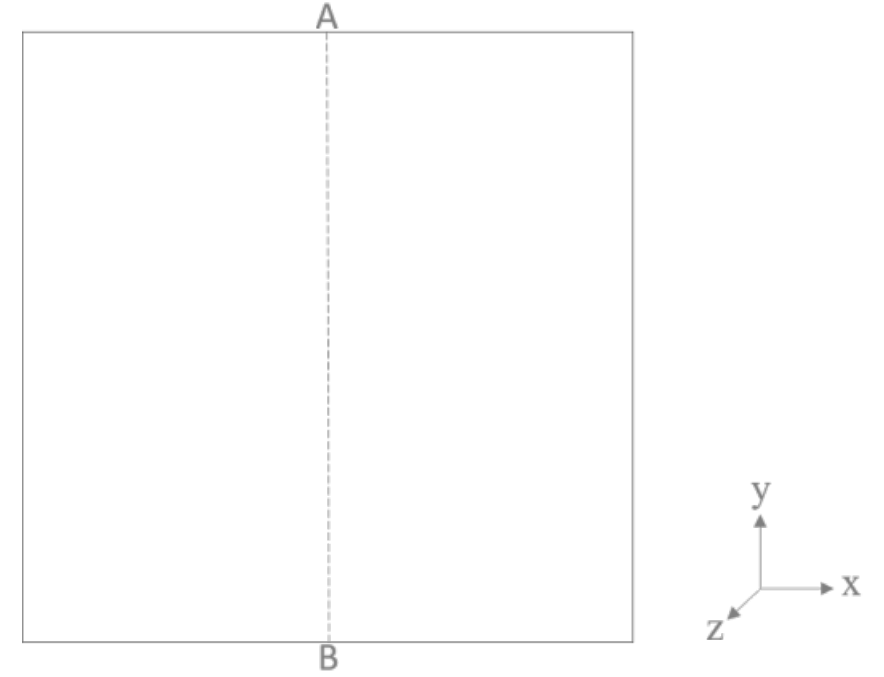
\includegraphics[width=200pt]{images/fig-eg-surf-deformer-1}
    \caption{Configuração inicial da superfície a ser deformada.~\cite{Muller}}\label{fig-eg-surf-deformer-1}
  \end{center}
\end{figure}


\begin{figure} [H]
  \begin{center}
    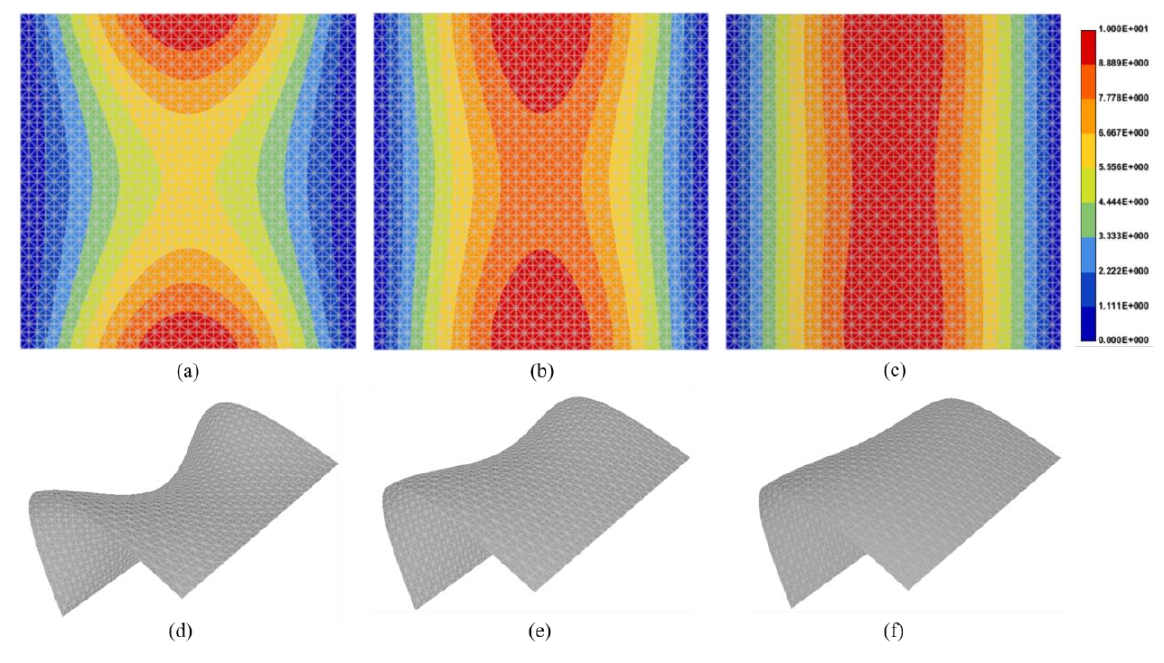
\includegraphics[width=\textwidth]{images/fig-eg-surf-deformer-2}
    \caption{Configuração deformada da superfície segundo as Lagrangeanas de 2ª ordem (a,d), 4ª ordem (b,e) e 6ª ordem (c, f). As figuras (a, b e c) representam os resultados na direção $z$, escala em metros.\cite{Muller}}\label{fig-eg-surf-deformer-2}
  \end{center}
\end{figure}

A Figura~\ref{fig-eg-surf-deformer-2} deixa clara as diferenças na deformação da superfície conforme a energia minimizada. De modo específico para a deformação de superfícies geológicas onde há um viés físico atrelado, a solução que minimiza a energia de mínima variação e que, portanto, resulta na mínima variação da curvatura é a que melhor se adequa ao comportamento previsto para este tipo de simulação.

O gráfico da Figura~\ref{fig-eg-surf-deformer-3} destaca o campo de deslocamentos em $z$ sobre o segmento $\overline{AB}$ da Figura~\ref{fig-eg-surf-deformer-1} para cada um dos três tipos de deformação mencionados.

\begin{figure} [H]
  \begin{center}
    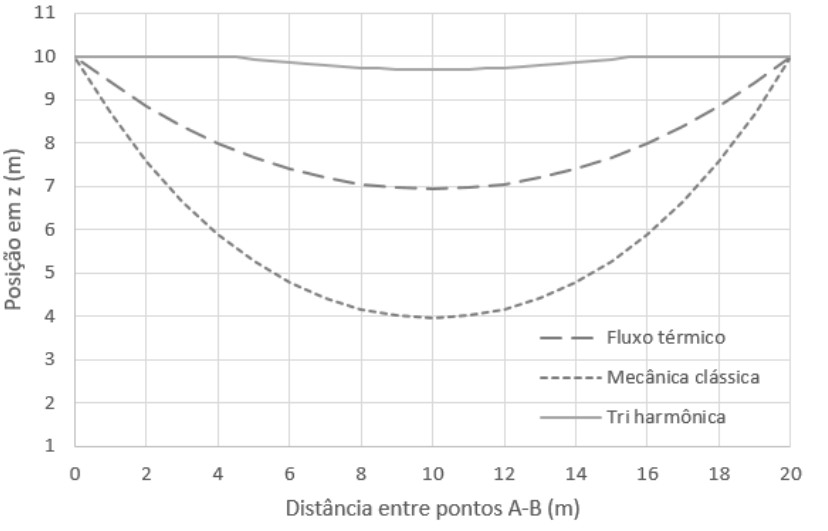
\includegraphics[width=250pt]{images/fig-eg-surf-deformer-3}
    \caption{Coordenada $z$ sobre o segmento $\overline{AB}$.\cite{Muller}}\label{fig-eg-surf-deformer-3}
  \end{center}
\end{figure}

Os procedimentos computacionais para os tipos de minimização de energia de superfície descritos nesta seção foram implementados por Müller e estão disponíveis na biblioteca \emph{MGeo Deformer}~\cite{Muller} do Sistema Recon.

\section{Preparação dos dados}
 
A metodologia mostrada anteriormente é capaz de realizar a deformação de superfície mediante conhecimento da posição inicial da mesma e também de informação de movimentação de pontos de controle, pontos estes que devem fazer parte do domínio da superfície. Desse modo, no contexto de restauração de seções no Sistema Recon, o mapeamento de superfície é obtido com a deformação desta superfície de acordo com parâmetros provenientes das seções. Em outras palavras, o mapeamento de superfície usa dados das seções como pontos de controle para se conseguir um comportamento equivalente no ambiente tridimensional. Essa é uma forma sucinta de descrever o modo como o mapeamento de superfície é feito. Nesta subseção serão apresentadas as etapas que permitem o uso do deformador de superfícies (\emph{MGeo Deformer}) com o intuito de se obter o mapeamento de superfícies.

Importante salientar que o ideal é que após a seção ter sido criada ocorra o mínimo de edição inicial nas linhas geradas. Isso é importante pois quanto melhor definida esteja a seção após o fatiamento (item~\ref{item-section-creation}), mais coerente com as superfícies tridimensionais estará o modelo como um todo. Edições nas linhas são comuns de acontecerem para que seja possível realizar a restauração da seção, entretanto, em caso de edições maiores ocorrerá o descasamento entre seção e superfícies e, nesta etapa, poderão haver incongruências.

\subsection{\textit{LMModels}}\label{lmmodels-surface-map}

O objetivo desta subseção é mostrar como obter informação de deslocamento dos horizontes entre etapas de restauração de uma seção geológica a partir de \textit{LMModels}. O deslocamento de pontos de horizonte é o dado principal vindo das seções para o mapeamento de deformações de horizontes, uma vez que as seções geológicas são cortes transversais planos de um conjunto de superfícies tridimensionais.

Como já visto, as \textit{LMModels} são linhas de mapeamento da seção baseadas em entidades geológicas. Estas linhas acompanham a movimentação tectônica na seção durante a restauração. Para esta etapa do trabalho, considera-se apenas as \textit{LMModels} de horizonte, ou seja, aquelas que tem como origem uma linha de horizonte, como as mostradas na Figura~\ref{fig-lmmodel-example}.

A movimentação tectônica da seção pode ser mensurada como uma diferença entre uma e outra etapa de restauração, mais especificamente, a distância entre os pontos de \textit{LMModels} correspondentes entre a etapa atual e a próxima.

A \textit{LMModel} em si não possui pontos geométricos, ela armazena apenas os índices dos nós do contorno da malha na extensão correspondente a uma linha de horizonte (Figura~\ref{fig-lmm-mesh-boundary}). Dessa forma, entre um cenário e outro da mesma seção, pode ocorrer uma edição na malha que pode alterar os nós do contorno e assim alterando o conjunto de índices que formam a \textit{LMModel}.

\begin{figure} [H]
  \begin{center}
    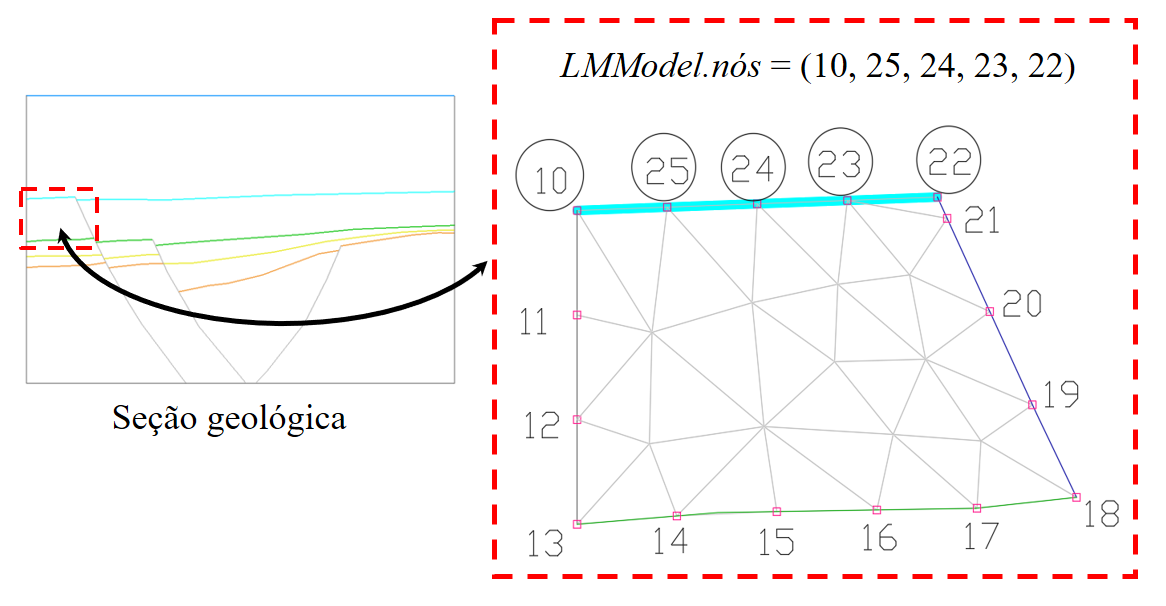
\includegraphics[width=310pt]{images/fig-lmm-mesh-boundary}
    \caption{Índices de nós que compõem uma parte de \textit{LMModels}.}\label{fig-lmm-mesh-boundary}
  \end{center}
\end{figure}

Para que se possa estabelecer uma relação direta de deslocamento entre pontos de uma \textit{LMModel} para diferentes cenários é necessário que se faça uma interpolação entre as malhas envolvidas. Esta ação serve para assegurar que se tenha um mesmo número de pontos formando a \textit{LMModel} correspondente ao longo da restauração de uma seção.

Para exemplificar melhor esse problema, considere a seção geológica da Figura~\ref{fig-lmm-interp1} (a) que destaca os pontos que formam a \textit{LMModel} do horizonte A (do topo). Considera-se que na etapa seguinte (cenário 2), houve uma transformação e uma edição na malha, com isso a \textit{LMModel} correspondente teve diminuição no número de pontos, como mostra a Figura~\ref{fig-lmm-interp1} (b).

\begin{figure} [H]
  \begin{center}
    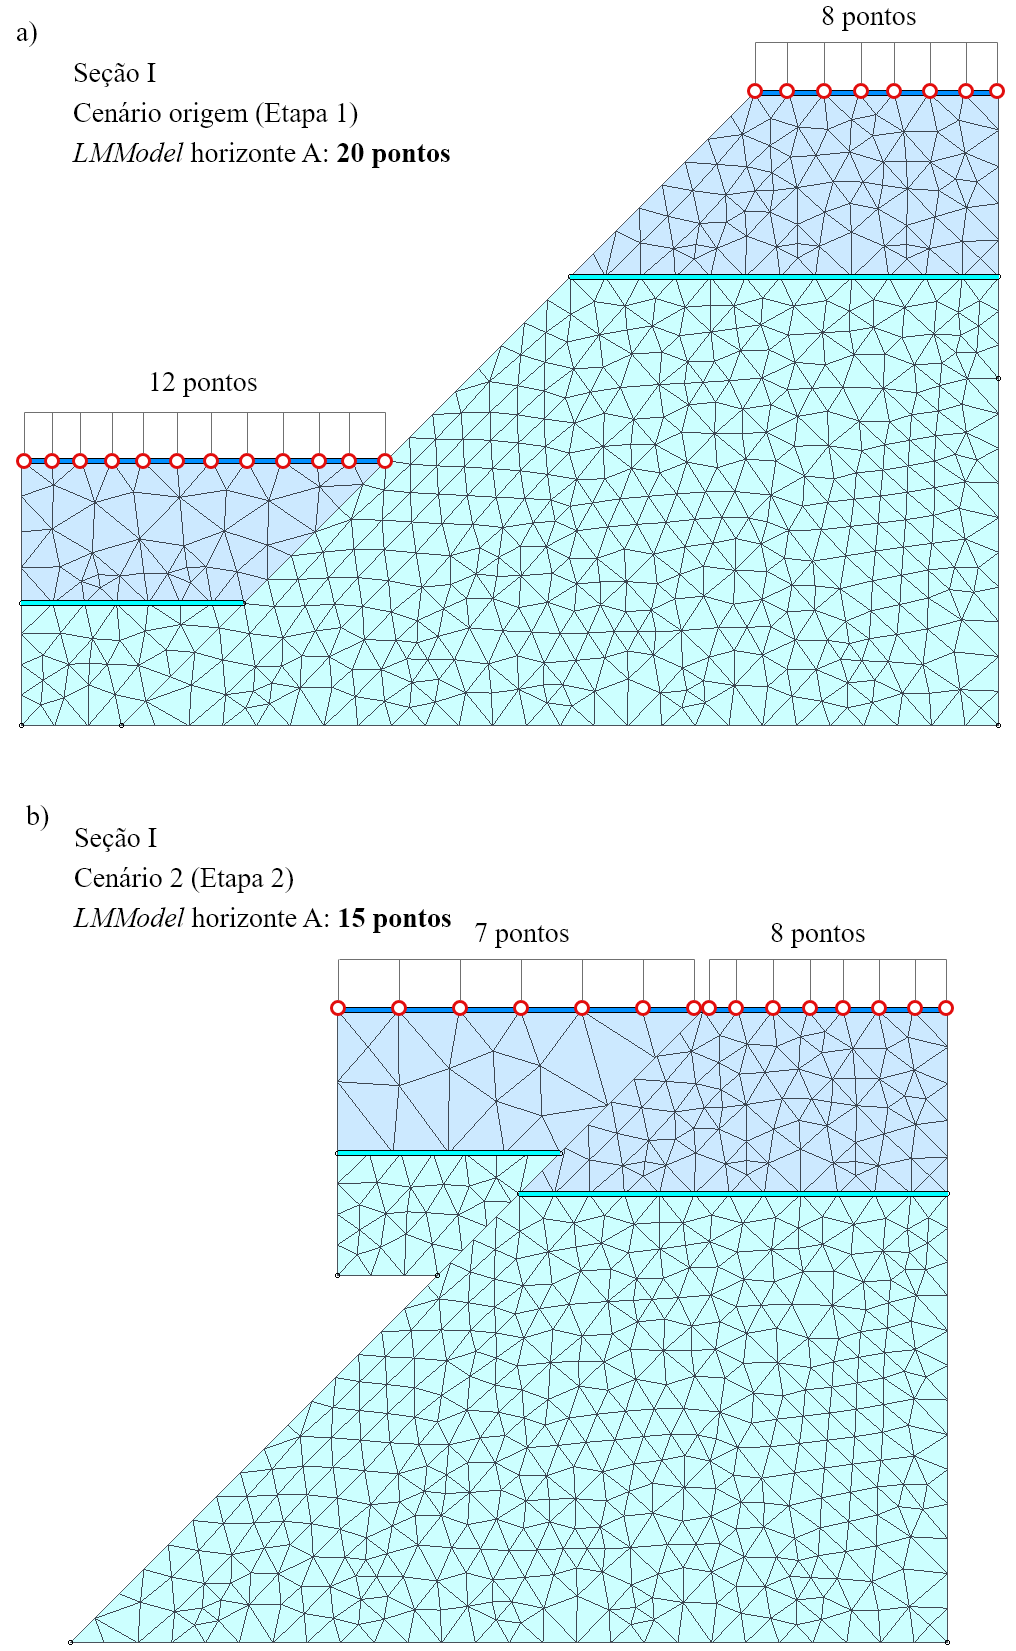
\includegraphics[width=300pt]{images/fig-lmm-interp1}
    \caption{\textit{LMModel} no cenário origem e cenário 2 com diferente número de pontos.}\label{fig-lmm-interp1}
  \end{center}
\end{figure}

Para que seja feito o cálculo de deslocamento entre as \textit{LMModels} destes cenários é necessário uma interpolação entre as malhas, como já dito. Essa interpolação fornece os pontos no cenário 2 que correspondem àqueles da \textit{LMModel} no cenário origem e assim ter dados para encontrar informações de deslocamento de uma etapa a outra.

Convencionou-se neste trabalho que a obtenção dos pontos de \textit{LMModels} toma como base para interpolação aquela criada no cenário origem, já que é um cenário mais restrito para edições após o início da restauração. Além disso, os pontos das \emph{LMModels} do cenário origem são usados com restrição para o \emph{remesh} da malha de superfície (item~\ref{surface-remesh}). Um esquema ilustrativo é visto na Figura~\ref{fig-lmm-interp2}.

\begin{figure} [H]
  \begin{center}
    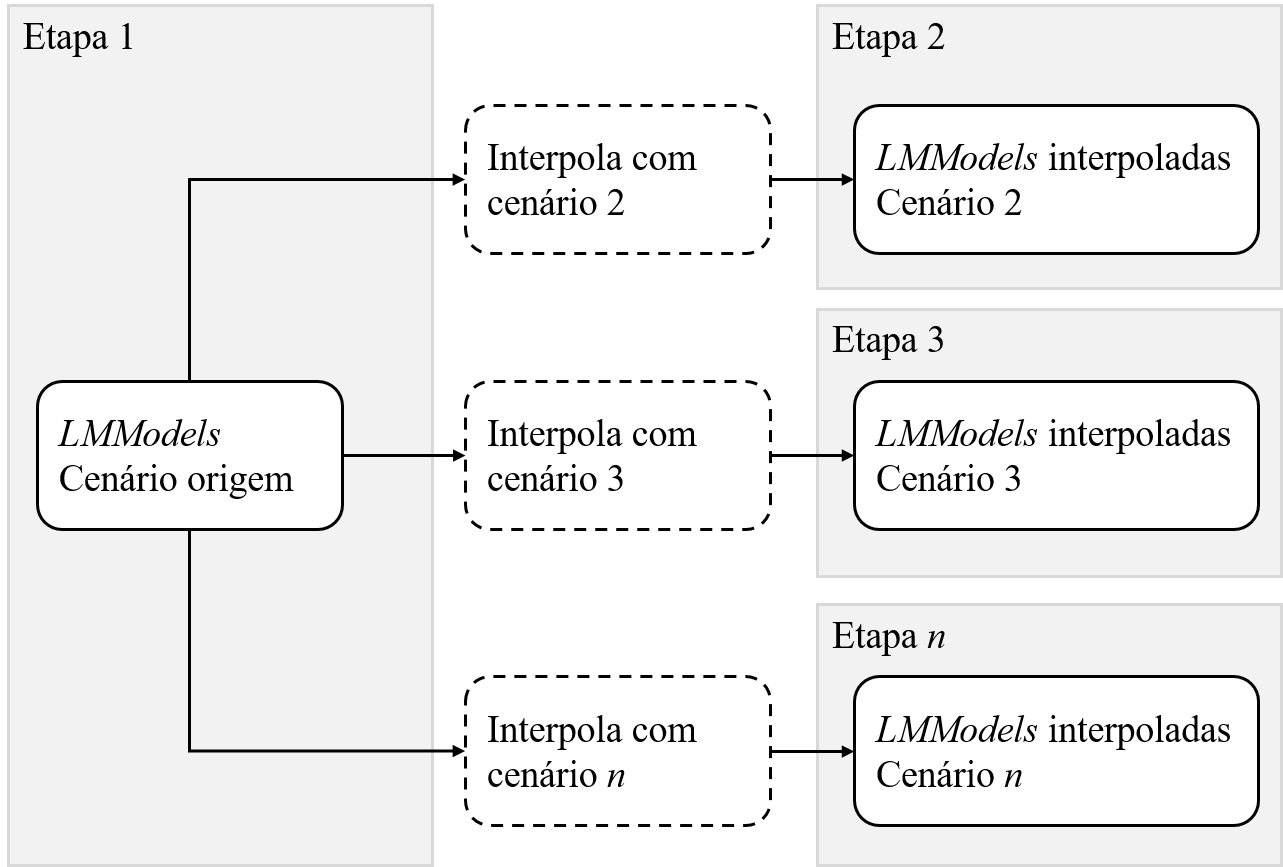
\includegraphics[width=350pt]{images/fig-lmm-interp2}
    \caption{Esquema de como obter número igual de pontos de \textit{LMModels} em diferentes cenários}\label{fig-lmm-interp2}
  \end{center}
\end{figure}

Ao se repetir esta ação para todas as seções que compõem o modelo, é possível criar uma estrutura de dados multidimensional com todos os pontos geométricos que formam as \textit{LMModels} a fim de facilitar o uso dessas informações. De maneira sucinta, esta estrutura é apresentada na Figura~\ref{fig-lmm-data-structure} como sendo análoga a uma matriz de 3 dimensões onde cada elemento é um conjunto de dois pontos cartesianos\footnote{os pontos nas malhas da seção estão em coordenadas bidimensionais, no entanto, ao criar esta estrutura de dados, todos os pontos são convertidos para coordenadas espaciais \textit{x}, \textit{y} e \textit{z} com base nas coordenadas UTM onde a seção se localiza.} e um dado booleano que indica se houve movimentação quando a diferença entre os pontos \textit{current} e \textit{next} é maior que uma dada tolerância.

\begin{figure} [H]
  \begin{center}
    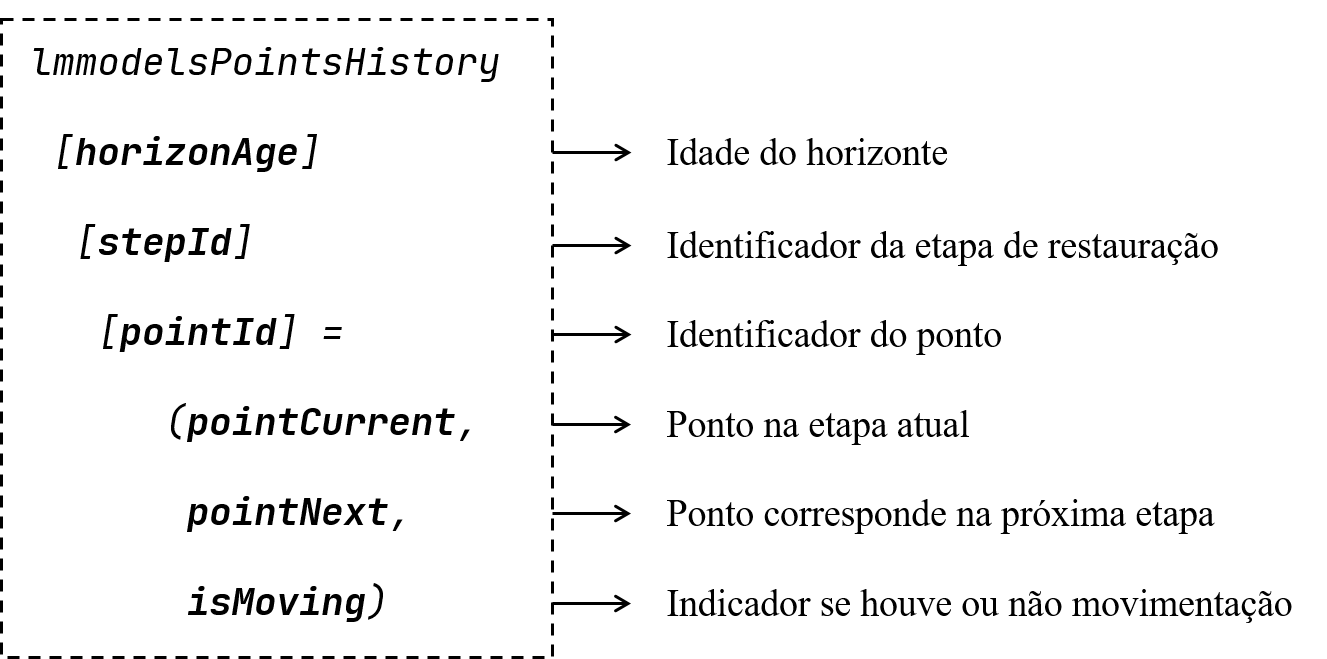
\includegraphics[width=350pt]{images/fig-lmm-data-structure}
    \caption{Estrutura de dados que armazena os pontos das \textit{LMModels} do modelo.}\label{fig-lmm-data-structure}
  \end{center}
\end{figure}

Importante ressaltar que é preciso ter o modelo já com todas as seções restauradas, uma vez que qualquer edição posterior nas seções, acarretará na necessidade de recriar a estrutura de dados de \textit{LMModels}.

\subsection{\textit{Remesh} da superfície}\label{surface-remesh}

No item~\ref{surface-mapping-metodology} foi apontada a necessidade de haver pontos de controle pertencentes à superfície, pontos estes que precisam ter sua posição final conhecida. Uma parte destes pontos de controle são as \textit{LMModels}, ou melhor, os pontos que representam o histórico de movimentação das \textit{LMModels}.

A interseção de um plano transversal a um conjunto de superfícies geológicas tridimensionais é o que produz a seção geológica, onde cada linha de horizonte é a representação de uma parte da superfície no plano bidimensional. Não por acaso, as \textit{LMModels} são mapeamentos dessas linhas de horizonte e, portanto, também mapeiam a superfície. No entanto, os pontos que formam a \textit{LMModel} foram gerados com base nas malhas de triângulos da seção e não possuem qualquer relação com os pontos que estão na superfície.

Com a finalidade de resolver esse problema é apresentado nesta subseção a necessidade de um \textit{remesh} (regeração da malha) que forma a superfície, cujo objetivo é produzir uma nova malha que contenha os pontos que formam as \textit{LMModels} das seções geológicas.

O \textit{remesh} é realizado com auxílio do algoritmo de regeração de malhas de superfícies considerando curvaturas proposto por Miranda \textit{et al.}~\cite{Miranda}. Os dados de entrada são as linhas de borda da superfície, uma malha de suporte representada por três funções generalizadas, criadas a partir da malha de suporte e um conjunto de pontos de restrição no domínio da superfície que, após o \textit{remesh} deverão fazer parte da malha.

As funções generalizadas são a maneira como a malha de suporte é representada e são apresentadas a seguir, de forma sucinta:

\renewcommand{\labelitemi}{•}
\begin{itemize}
  \item 1ª função: recebe um ponto da superfície como entrada e devolve o tamanho característico da aresta de um triângulo equilátero ideal na posição desse ponto. O cálculo desse tamanho envolve o uso de uma estrutura de dados \textit{octree}\footnote{Uma estrutura de árvore onde cada nó pode possuir oito filhos e representa a subdivisão do espaço em oito octantes~\cite{Donald}.} que fornece um refinamento de tamanho de acordo com a curvatura da superfície.
  \item 2ª função: calcula o ponto ideal que irá formar um novo triângulo de acordo com uma dada aresta no processo de contração de contorno de geração da malha. Além da aresta, são passados à função a altura do triângulo e um vetor unitário na direção perpendicular à aresta que será usado para definir o plano de interseção com a superfície e assim encontrar o ponto ideal.
  \item 3ª função: usada para melhoria na malha após a suavização. Recebe um ponto qualquer e retorna o ponto mais próximo pertencente à malha da superfície de suporte. Com a suavização, alguns nós mudam de lugar e podem acabar fora da superfície, ocorrendo isso, esta terceira função é utilizada para trazer de volta os pontos distantes. 
\end{itemize}

O algoritmo utiliza avanço de fronteira na primeira fase e faz uso da 1ª e 2ª funções para determinar a primeira versão da nova malha. Após isso começa a etapa de melhoria com suavização e em paralelo, o uso da 3ª função~\cite{Miranda}. O resultado final é uma malha com mais elementos em regiões de alta curvatura, como mostra a Figura~\ref{fig-remesh} onde as imagens (a) e (b) são as superfícies de suporte e as imagens (c) e (d) suas versões regeradas, respectivamente.

\begin{figure} [H]
  \begin{center}
    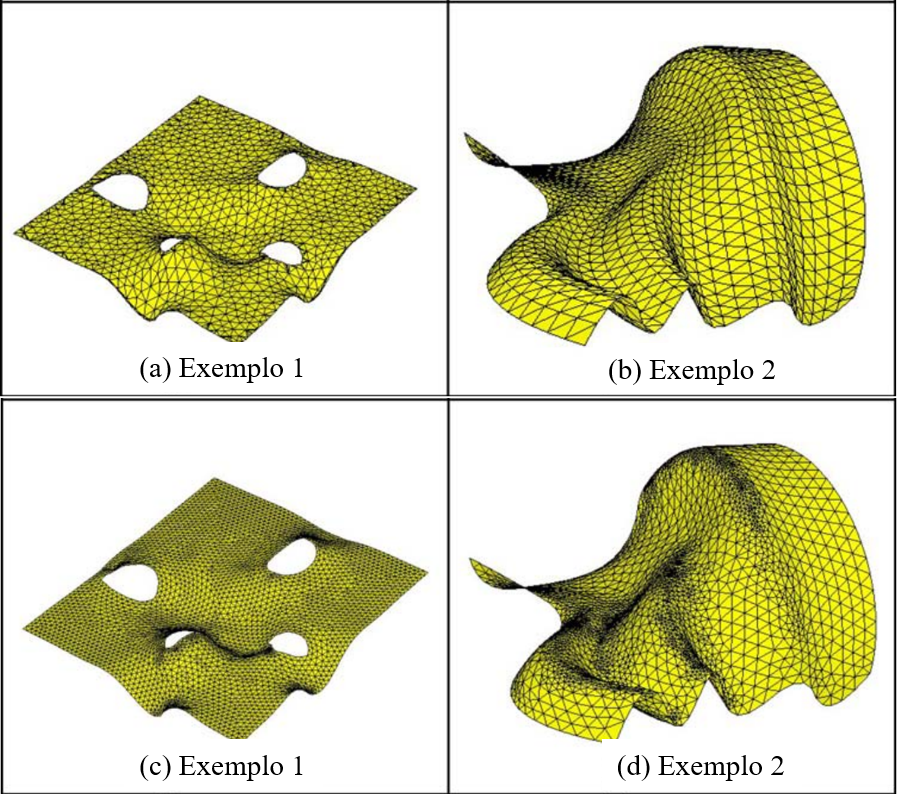
\includegraphics[width=350pt]{images/fig-remesh}
    \caption{Exemplo de resultado obtido com algoritmo de \textit{remesh}~\cite{Miranda}.}\label{fig-remesh}
  \end{center}
\end{figure}

Os pontos de restrição usados para a regeração da malha de superfície são as \textit{LMModels} da seção, portanto, passam a ser os pontos de controle da superfície geológica. Uma vez que os pontos que formam as \textit{LMModels} são todos iguais em número, pois tomam o cenário origem da \textit{EtapaMS} inicial e são interpolações com os cenários seguintes, o \textit{remesh} pode ser feito nesta \textit{EtapaMS} inicial e essa malha ser mantida para todo o restante do processo.

De uma \textit{EtapaMS} à outra, com as \textit{LMModels}, é possível ter o deslocamento das linhas de horizontes, por exemplo. Sendo os pontos das \textit{LMModels} nós da malha da superfície, esses nós passam a ter informação de posição final definida. Sendo assim, já seria possível realizar a deformação da superfície conforme metodologia já apresentada, pois o principal requisito está satisfeito. No entanto, se tratando do mapeamento de uma superfície que, num modelo geológico de multisseções, precisa estar coerente com o que ocorre nas seções, mais algumas restrições precisam ser impostas conforme descrito nas subseções a seguir.

\subsection{Definição das bordas origem/destino}

Na restauração de seções um dos principais objetivos é a eliminação do rejeito de falha, principalmente se tratando de modelos de tectônica distensiva onde há a presença de blocos divididos por essas falhas~\cite{Santi}. Nestes modelos, geralmente se quer movimentar um bloco sobre uma linha de falha até um certo ponto, de modo que a camada do topo esteja alinhada com a sua correspondente no bloco vizinho. A Figura~\ref{fig-section-horizon-restored} mostra uma seção com um horizonte restaurado com o uso da transformação \quotes{move sobre falha}.

\begin{figure} [H]
  \begin{center}
    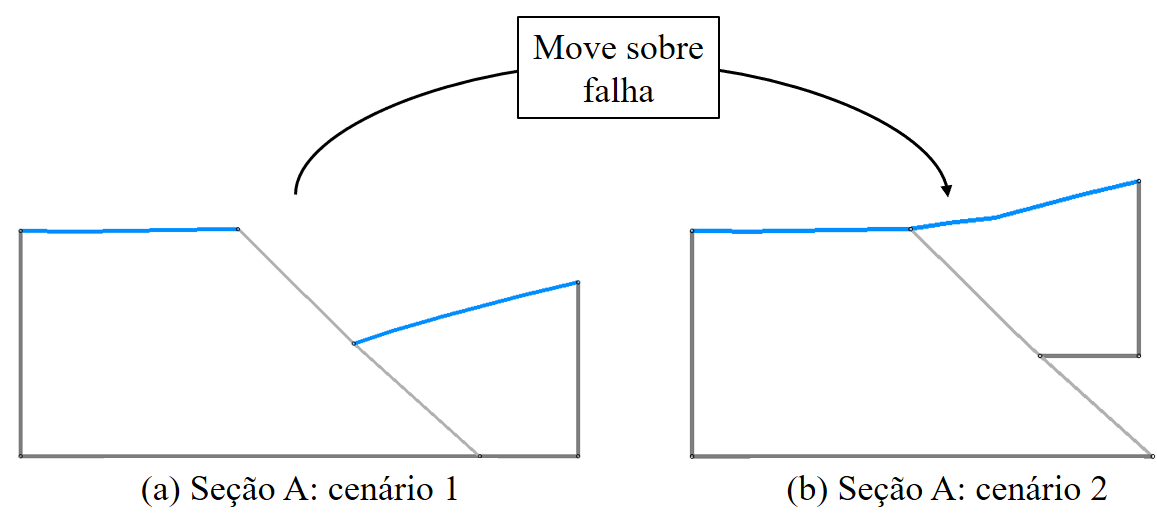
\includegraphics[width=350pt]{images/fig-section-horizon-restored}
    \caption{Restauração de horizonte em uma seção geológica através de uma transformação.}\label{fig-section-horizon-restored}
  \end{center}
\end{figure}

Esta ação de movimentar uma porção da seção até um certo limite é um comportamento necessário no mapeamento de superfícies, isto é, o mapeamento de superfícies precisa respeitar um limite de movimentação análogo àquele adotado na seção.

Em geral, no uso do Sistema Recon, uma \textit{EtapaMS} representa um marco geológico ocorrido em todas as seções do modelo simultaneamente. O que para este trabalho convencionou-se que seja uma restauração do rejeito de uma falha ou uma descompactação de topo restaurado. Logo, para o mapeamento de superfícies, é necessário que cada \textit{EtapaMS} represente a restauração de uma falha (ou descompactação) ocorrida ao mesmo tempo em todas seções onde tal falha atravesse. Pois, como nas seções, as superfícies de horizontes também estão com as falhas cruzando seu domínio, como mostra a Figura~\ref{fig-surfaces-horizon-faults}.

\begin{figure} [H]
  \begin{center}
    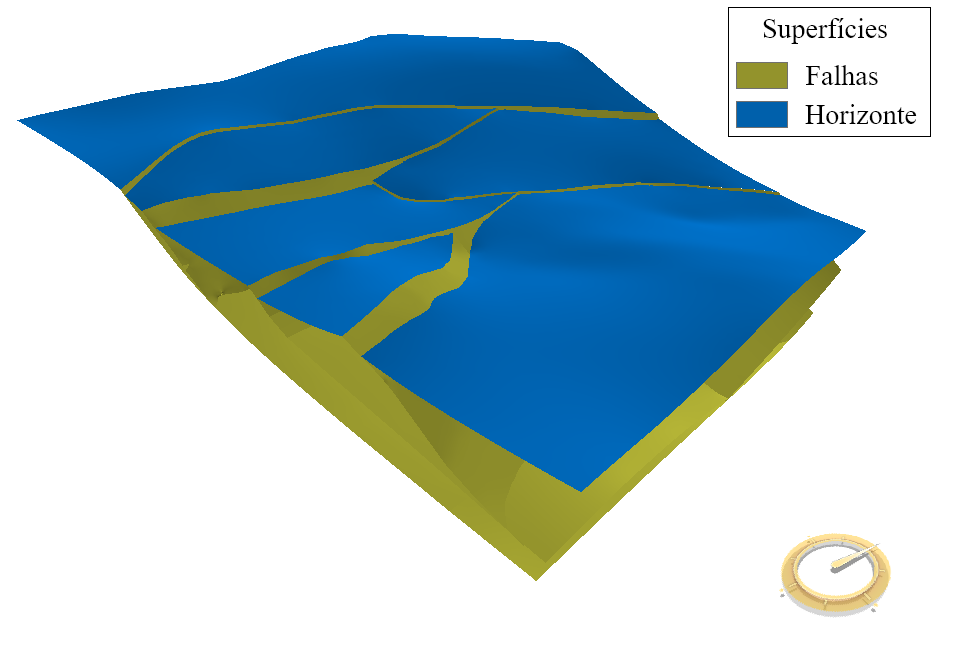
\includegraphics[width=310pt]{images/fig-surfaces-horizon-faults}
    \caption{Vista 3D de uma superfície de horizonte atravessada por várias superfícies de falhas.}\label{fig-surfaces-horizon-faults}
  \end{center}
\end{figure}

Como forma de definir limites de movimentação na deformação da superfície, pode-se indicar bordas de origem e destino da superficie. Esse é um procedimento análogo à movimentação de bloco ocorrida nas seções ao longo de uma falha. Essa indicação servirá ainda para auxiliar na definição da direção de movimentação das partes envolvidas em uma dada \textit{EtapaMS} na deformação da superfície.

Esse mapeamento de superfície é feito passo a passo conforme o número de \textit{EtapasMS} do modelo. Com a \textit{EtapaMS} vem a informação de qual falha está sendo restaurada\footnote{Para o caso de descompactação, a etapa de selecionar bordas não é necessária.}, com isso é necessário selecionar e marcar as bordas da superfície na região da falha para assim guiar a direção e o limite de movimentação durante a deformação da mesma.

O processo em mais detalhes pode ser explicado com o auxílio do exemplo de um modelo geológico simplificado, mostrado na Figura~\ref{fig-select-borders-1}, onde há uma superfície de horizonte, uma falha, 3 seções transversais e cuja \textit{EtapaMS} corrente é a de restauração dessa falha.

\begin{figure} [H]
  \begin{center}
    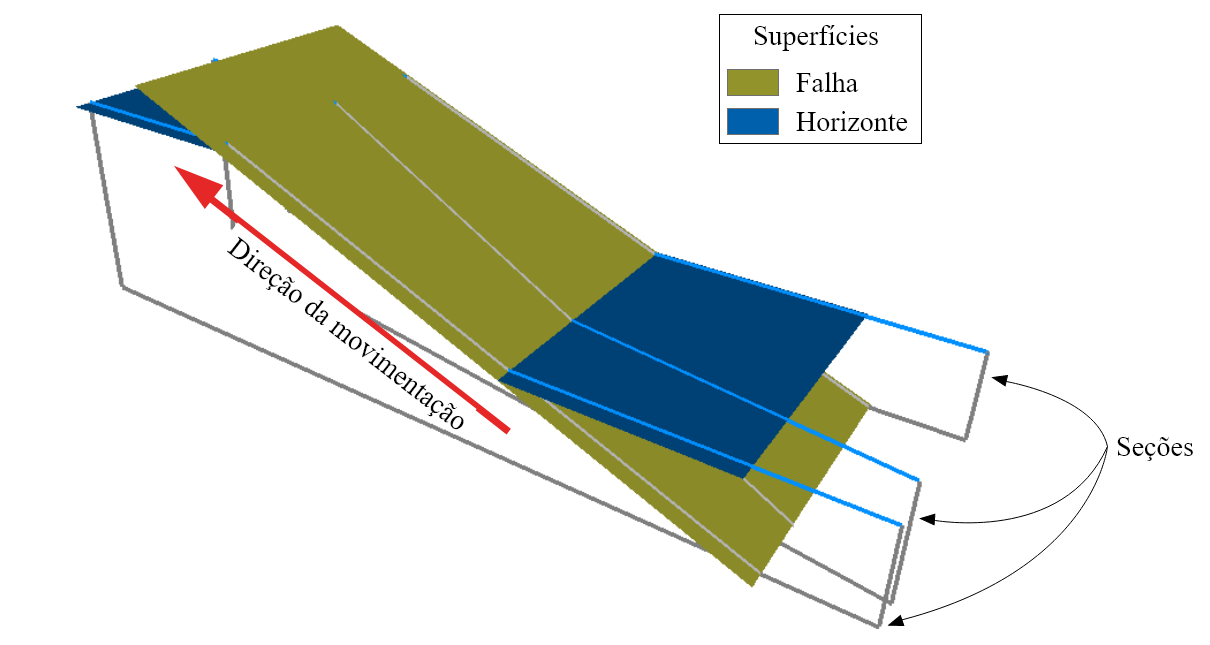
\includegraphics[width=350pt]{images/fig-select-borders-1}
    \caption{Modelo geológico tridimensional simplificado.}\label{fig-select-borders-1}
  \end{center}
\end{figure}

Neste caso, tal qual ocorre nas seções, o pedaço de superfície de horizonte à direita na imagem é que deve se movimentar e ir de encontro à parte que está do lado esquerdo. Logo, o pedaço à direita possui a borda de origem e o da esquerda, a borda de destino, como mostra a Figura~\ref{fig-select-borders-2}.

\begin{figure} [H]
  \begin{center}
    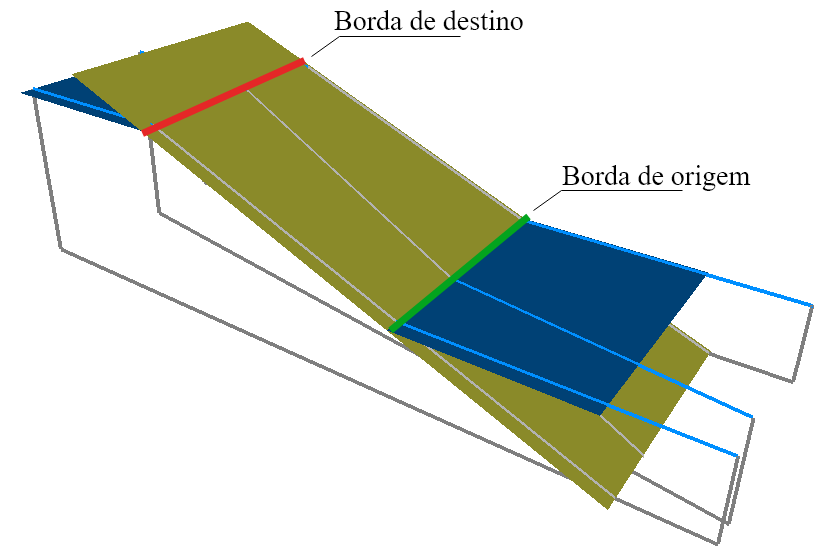
\includegraphics[width=300pt]{images/fig-select-borders-2}
    \caption{Indicação da localização das curvas origem e destino}\label{fig-select-borders-2}
  \end{center}
\end{figure}

A partir dessa marcação, que na prática ocorre nos pontos do contorno da malha da superfície, são calculados os vetores direção de cada ponto da borda de origem que deverão se deslocar até interceptar a linha poligonal formada pelos pontos da curva de destino. Esse algoritmo, se baseia na direção das seções no plano \textit{xy}, como numa vista de mapa. Observa-se pela Figura~\ref{fig-select-borders-3}, com vista em mapa, que nesse exemplo a seção do meio (seção S2) está inclinada em relação às outras seções que são paralelas entre si.

\begin{figure} [H]
  \begin{center}
    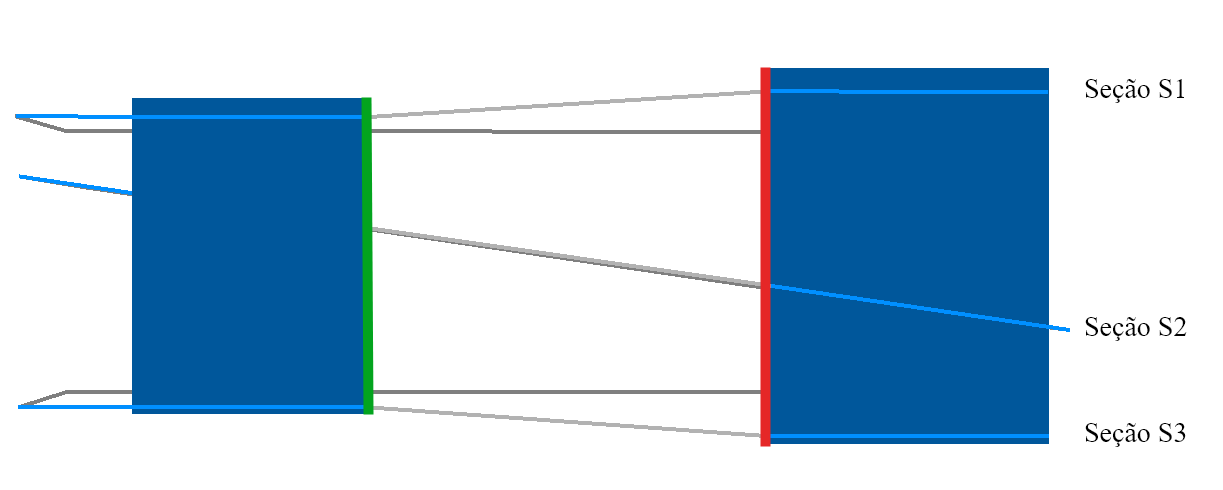
\includegraphics[width=350pt]{images/fig-select-borders-3}
    \caption{Vista de mapa do modelo para evidenciar a direção das seções.}\label{fig-select-borders-3}
  \end{center}
\end{figure}

A fim de dar mais detalhes sobre como o algoritmo de cálculo das direções funciona, considere a ilustração na Figura~\ref{fig-select-borders-4} com base nas seções e nas bordas de origem e destino desprezando o eixo \textit{z}:

\begin{figure} [H]
  \begin{center}
    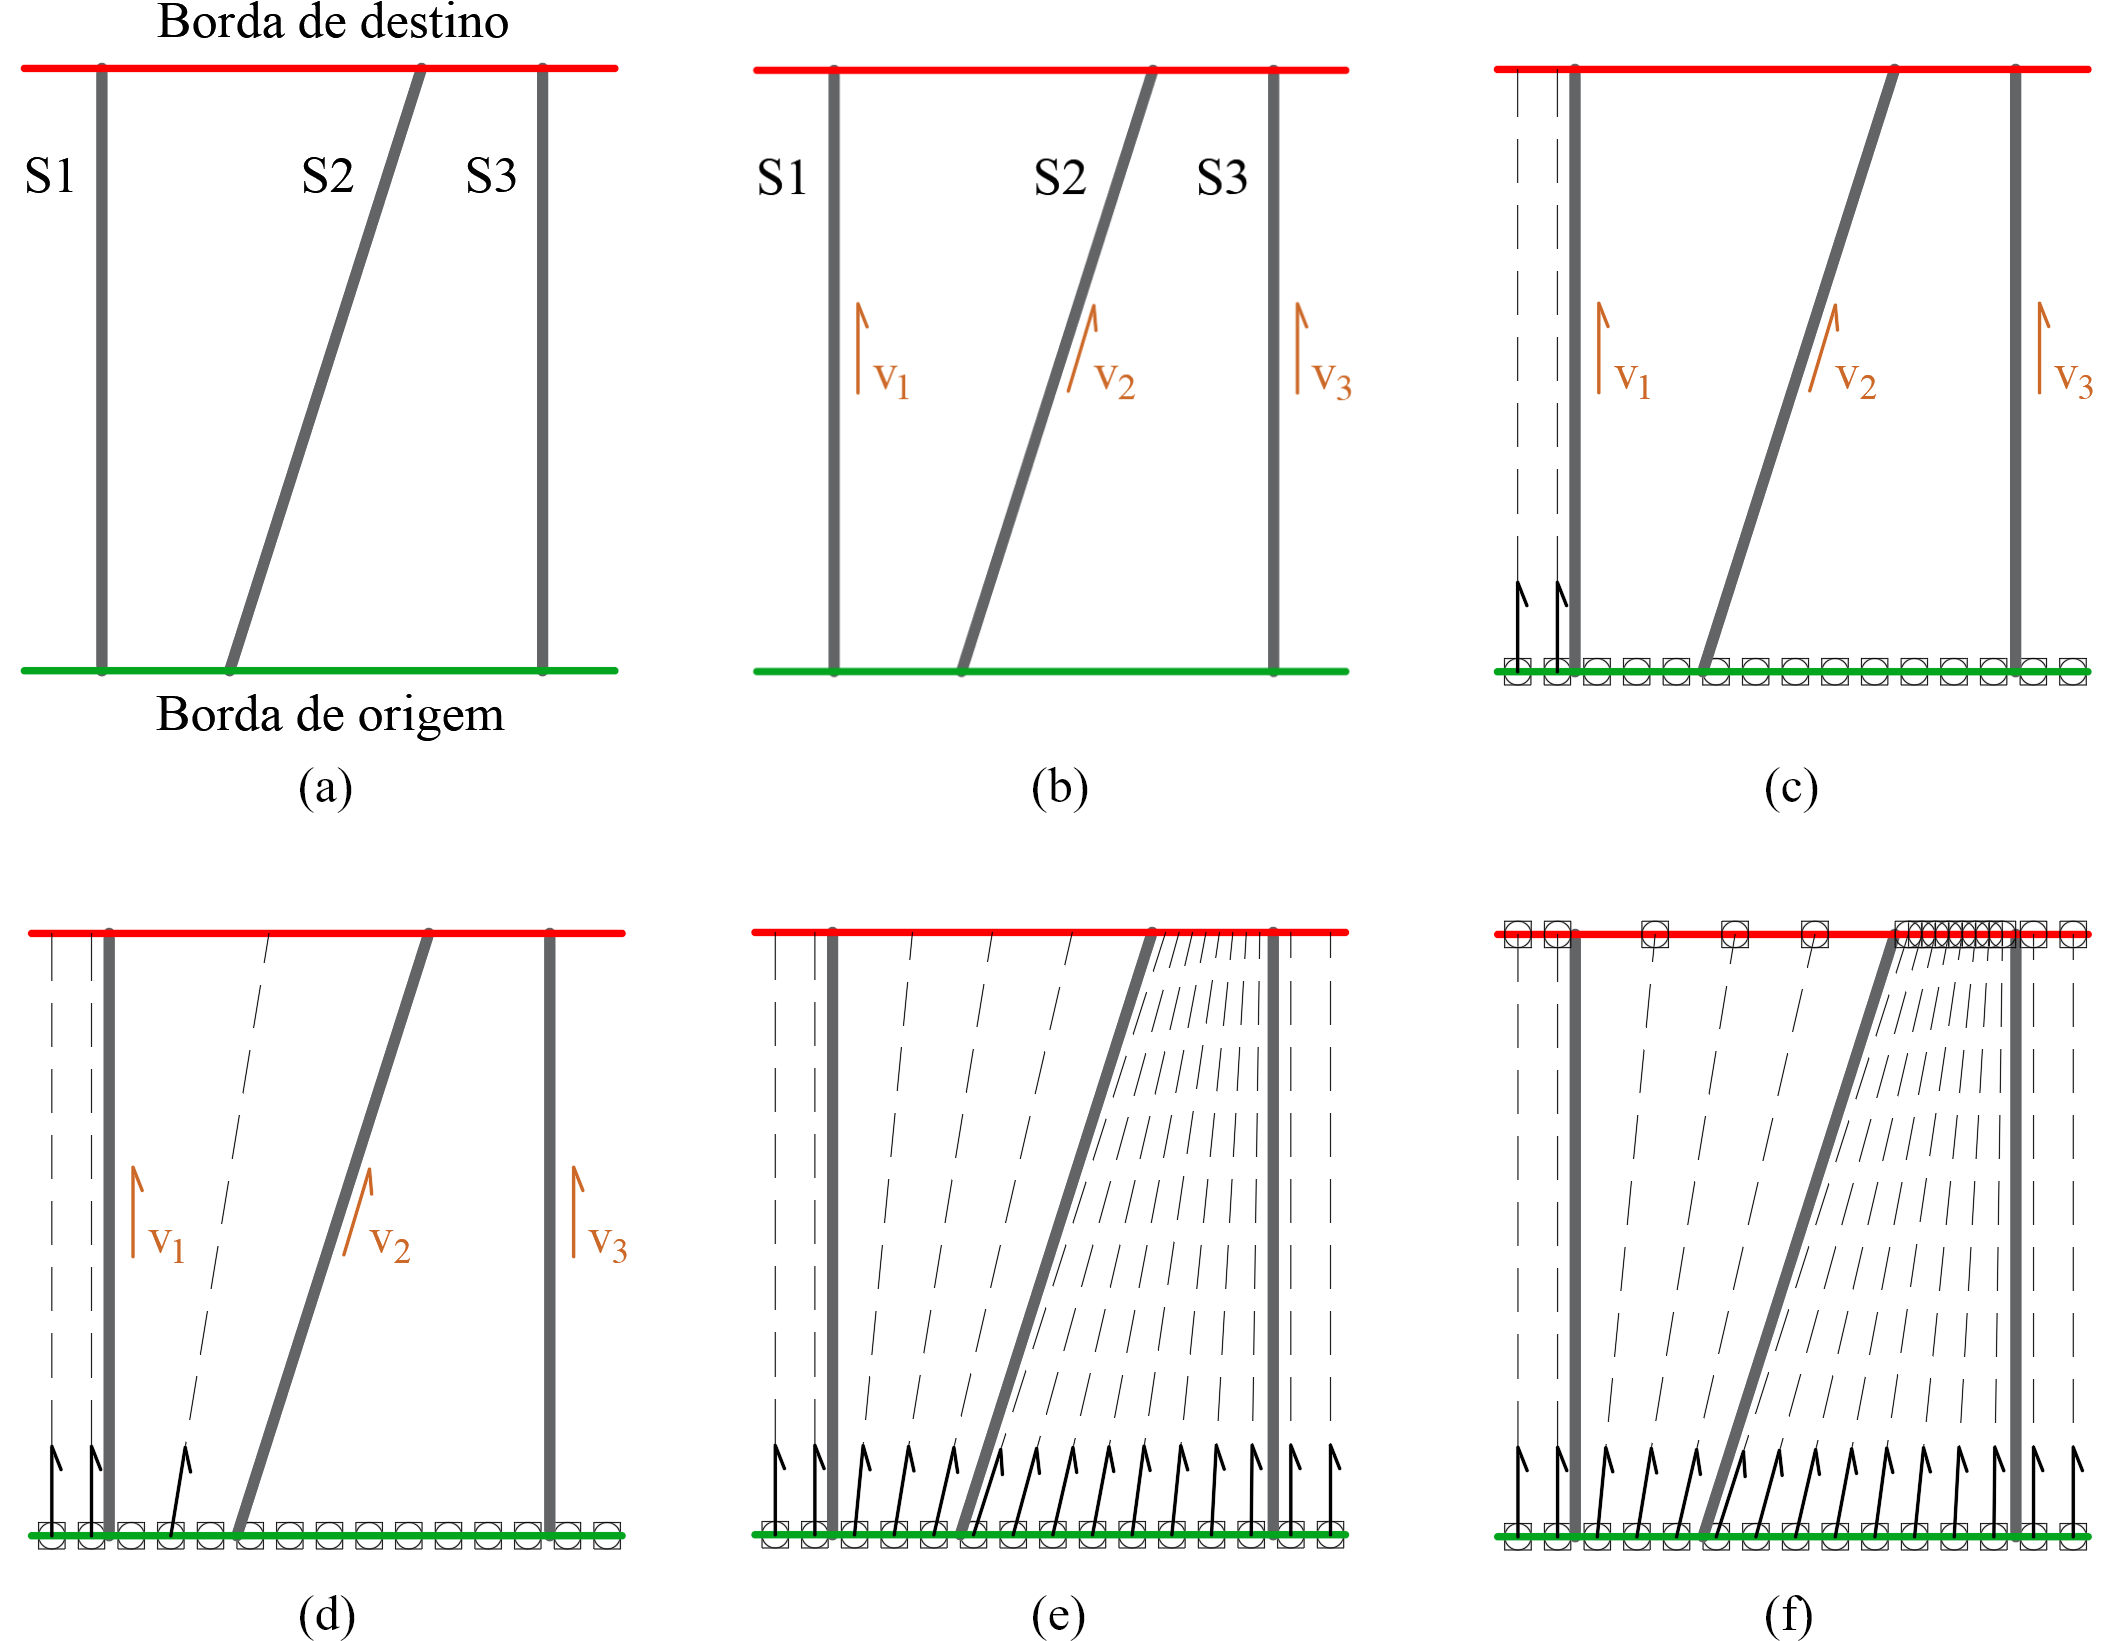
\includegraphics[width=370pt]{images/fig-select-borders-4}
    \caption{Procedimento para cálculo da direção dos pontos da borda de origem para a borda de destino.}\label{fig-select-borders-4}
  \end{center}
\end{figure}

Na Figura~\ref{fig-select-borders-4}-a estão representadas as bordas origem e destino e também as seções geológicas que cortam essas bordas. A primeira parte do procedimento (Figura~\ref{fig-select-borders-4}-b) consiste em calcular o vetor unitário que tem a mesma inclinação das seções. Isso é feito com dados dos pontos de interseção da seção com as superfícies de falha na região das bordas. Com as direções das seções definidas, se inicia o cálculo da direção dos pontos da superfície na borda de origem (Figura~\ref{fig-select-borders-4}-c), cada ponto à esquerda da primeira seção recebe a mesma direção desta. Para pontos de borda que estão entre seções (Figura~\ref{fig-select-borders-4}-d), a direção é calculada como uma combinação linear das direções das seções vizinhas, com base na distância do ponto até a interseção destas seções com a borda de origem. Prossegue-se com o cálculo de todas as direções dos pontos de borda (Figura~\ref{fig-select-borders-4}-e) e assim como nos pontos à esquerda da primeira seção, os pontos que estão logo ao lado direito da última seção recebem a direção desta. Por último (Figura~\ref{fig-select-borders-4}-f), são calculados os pontos de destino dos pontos da borda de origem, com o vetor direção, é traçado uma reta até interceptar (ou não) a poligonal formada pela borda de destino, caso haja a interseção, esse ponto é salvo como destino do ponto da borda de origem.

Assim como os pontos das \textit{LMModels}, cada ponto da borda de origem que encontrar um ponto correspondente na borda de destino da superfície passa a ser um ponto de controle, pois possui uma posição final definida, que irá auxiliar na deformação da superfície ao ser executado o mapeamento.

Importante salientar que a definição das bordas origem e destino só é requerida para a superfície que está no topo do modelo pois a restrição na movimentação se baseia em unir partes do horizonte do topo, assim como ocorre nas seções.

\subsection{Definição de movimentação dos nós da superfície}

Outra característica presente na restauração de seções com falhas distensivas é que, conforme a metodologia de restauração, o bloco alto permanece parado enquanto o bloco baixo se movimenta deslizando-se pela linha de falha (Figura~\ref{fig-hang-foot-wall}).

\begin{figure} [H]
  \begin{center}
    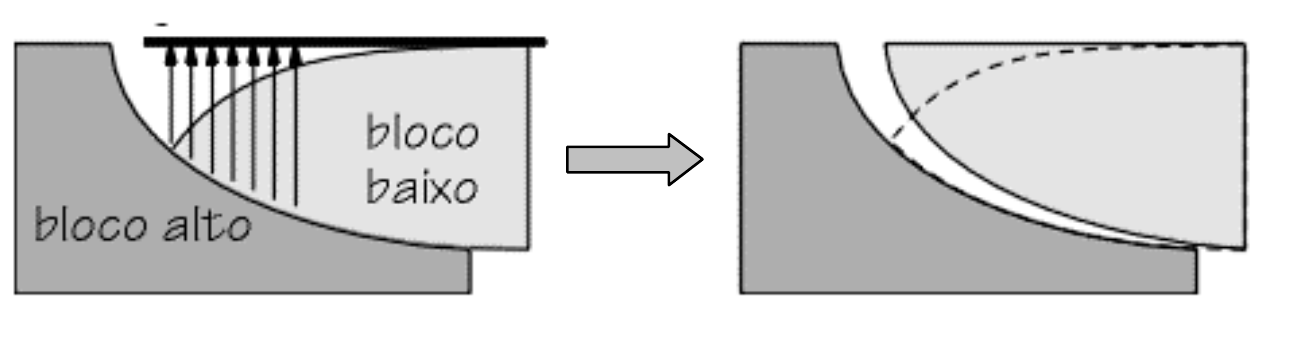
\includegraphics[width=300pt]{images/fig-hang-foot-wall}
    \caption{Movimentação do bloco baixo sobre o bloco alto.~\cite{Santi}}\label{fig-hang-foot-wall}
  \end{center}
\end{figure}

Este é um caso comum que ocorre no processo de restauração, onde quase sempre uma parte da seção se movimenta em relação a uma parte que fica imóvel. Assim como discutido na subseção anterior, este comportamento também precisa ser levado para o mapeamento de superfície a fim de manter a coerência no ambiente tridimensional, uma vez que trata-se do mesmo modelo.

Na deformação da superfície, na definição do mapeamento da mesma, é preciso indicar, a cada etapa, quais pontos da superfície irão se movimentar e quais permanecerão imóveis. De imediato, é correto afirmar que os pontos das \textit{LMModels} que possuem posição final diferente da posição inicial e também os pontos da borda de origem que têm um correspondente na borda de destino irão se movimentar. Também se pode garantir que os pontos das \textit{LMModels} que não mudam de uma \textit{EtapaMS} para outra e os pontos da borda de destino ficarão imóveis.

Todos estes pontos fazem parte da malha da superfície (após o \textit{remesh}) e são eles os primeiros a receber essa marcação de \quotes{move} ou \quotes{não move}. Para o restante dos pontos a marcação é feita com o auxílio do algoritmo de \textit{breadth-first search} (BFS) ou busca em largura~\cite{Nilsson}. Essa BFS roda sobre um grafo construído com base na malha da superfície. 

Para criar esse grafo, ocorre uma iteração por todos as arestas da malha da superfície para coleta dos índices de seus dois vértices, $v_i$ e $v_j$. Cada vértice no grafo possui uma lista de outros vértices que são seus adjacentes. Na lista do primeiro vértice $v_i$ é adicionado o segundo vértice $v_j$. Assim, no grafo, cada nó possui uma lista de seus nós adjacentes.

Com o grafo pronto é preciso identificar os primeiros a receberem uma marcação de \quotes{move} ou \quotes{não move}, sumarizando:

\renewcommand{\labelitemi}{•}
\begin{itemize}
  \item todos os nós da borda de origem são marcados como \quotes{move};
  \item todos os nós da borda de destino são marcados como \quotes{não move};
  \item Os pontos das \textit{LMModels} (que são parte da superfície) são marcados como: \quotes{move} se o correspondente na próxima \textit{EtapaMS} estiver em outra posição e \quotes{não move}, caso contrário (não há deslocamento).
\end{itemize}

A BFS é um algoritmo que realiza uma busca a partir de todos os nós do primeiro nível, daí então vai para o segundo nível que são todo os nós vizinhos do primeiro e assim por diante~\cite{Nilsson}, como mostrado na Figura~\ref{fig-bfs}, sempre visitando todos os nós do nível corrente antes de incrementar a posição na profundidade dos dados.

\begin{figure} [h]
  \begin{center}
    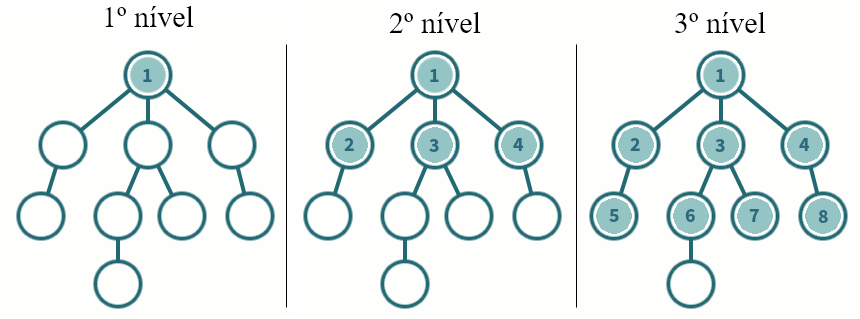
\includegraphics[width=350pt]{images/fig-bfs}
    \caption{Busca em largura ou BFS.~\cite{BFS}}\label{fig-bfs}
  \end{center}
\end{figure}

Neste caso, o primeiro nível é formado por todos os pontos inicialmente marcados, seja com \quotes{move} ou \quotes{não move}, inicia-se então a iteração com a BFS onde cada nó visitado posteriormente recebe a mesma marcação do vizinho anterior. Este laço se repete até que todos os nós da superfície tenham sido visitados.

\section{Exemplos e resultados}

Nesta seção são apresentados alguns exemplos para demonstrar o mapeamento de superfícies com base na restauração de seções. Todo o processo foi feito em uma versão experimental do Sistema Recon onde os desenvolvimentos deste trabalho têm sido implementados.

\subsection{Exemplo: modelo geológico simplificado}

Como já apresentado na Figura~\ref{fig-select-borders-1}, este é um modelo produzido manualmente que serviu para a experimentação na fase inicial do desenvolvimento deste trabalho. Ele, de forma mais completa, apresenta três seções paralelas, dois horizontes e uma falha (Figura~\ref{fig-example-1-1}). Também possui apenas uma etapa de restauração. 

\begin{figure} [H]
  \begin{center}
    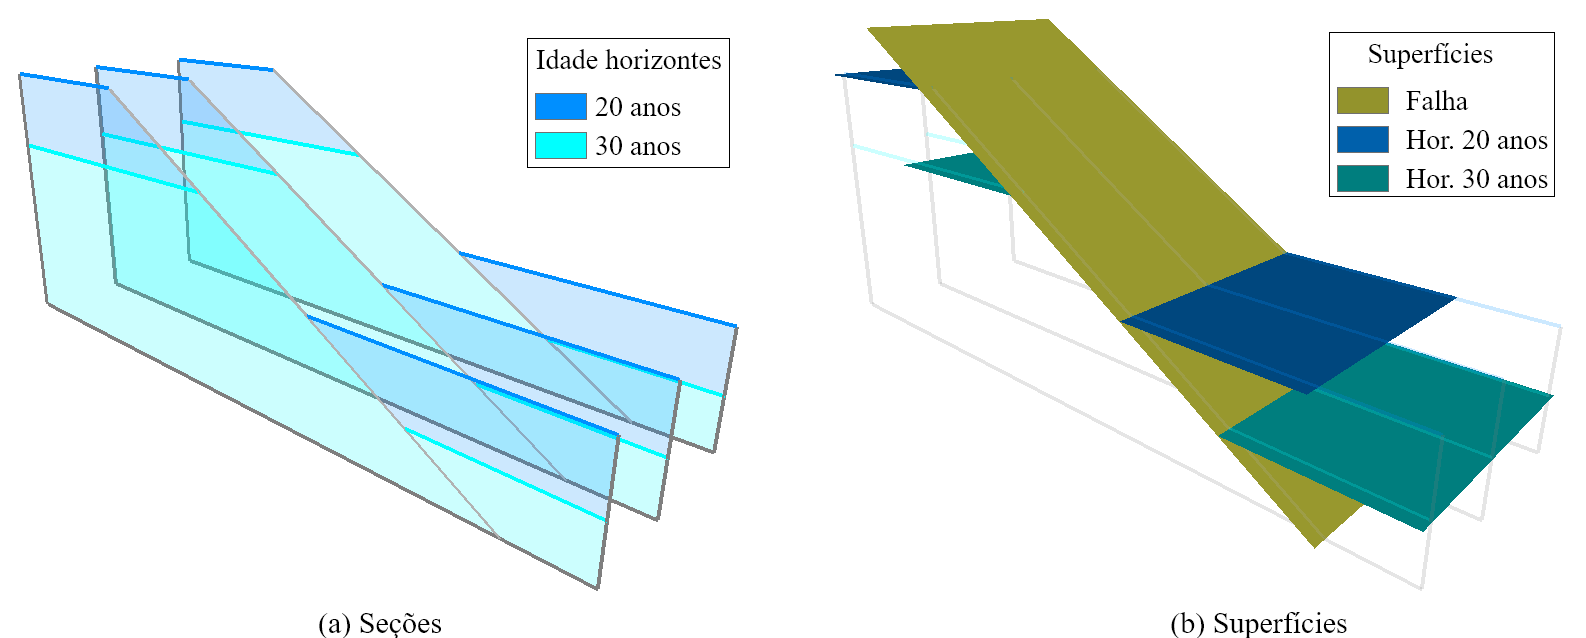
\includegraphics[width=\textwidth]{images/fig-example-1-1}
    \caption{Vista tridimensional das (a) seções e (b) superfícies do modelo simplificado.}\label{fig-example-1-1}
  \end{center}
\end{figure}

O modelo já se encontra com suas seções geológicas restauradas, com isso então pode-se começar com a criação das \textit{LMModels} e sua estrutura de dados com a forma apresentada na Figura~\ref{fig-lmm-data-structure}. A representação visual das \textit{LMModels} criadas pode ser vista na Figura~\ref{fig-example-1-2}.

\begin{figure} [h]
  \begin{center}
    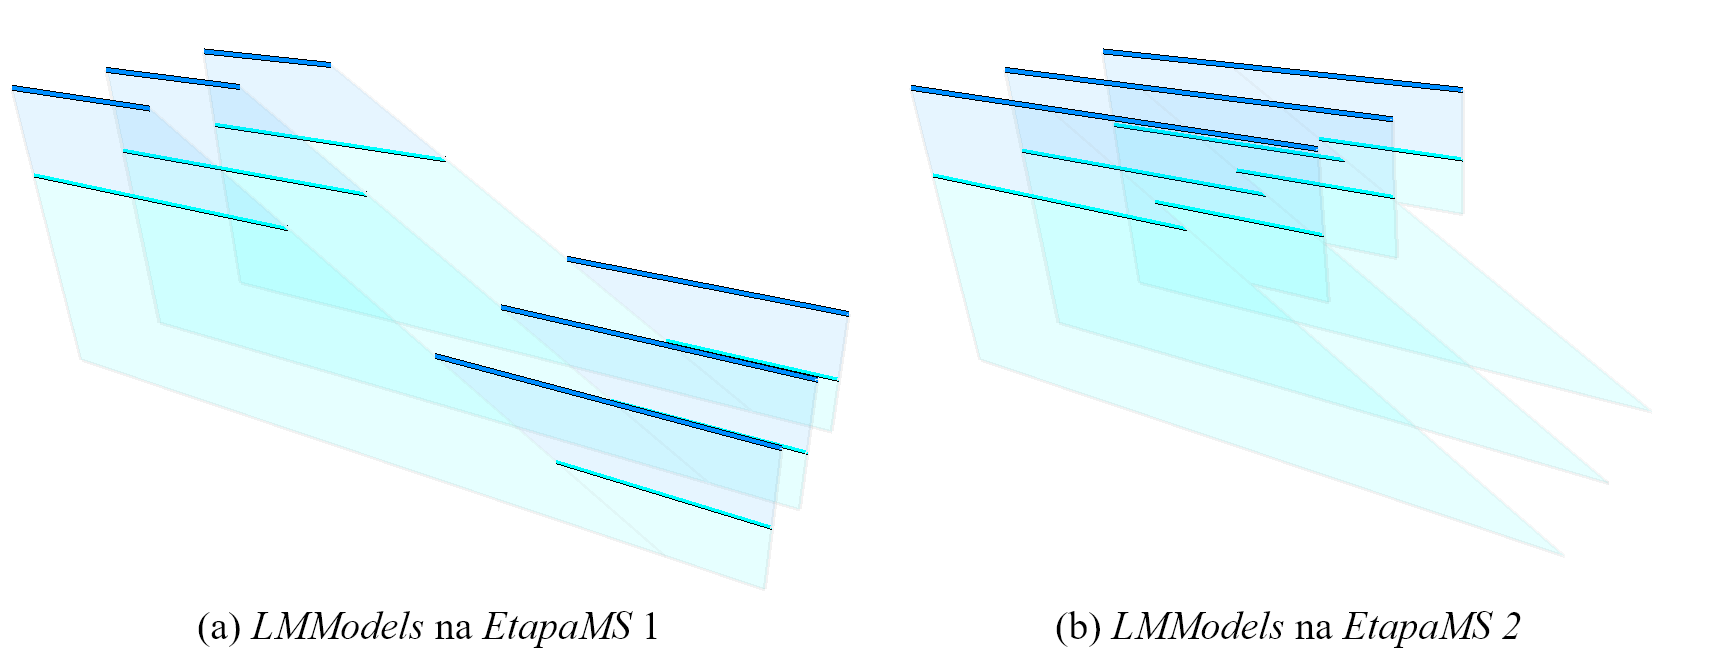
\includegraphics[width=\textwidth]{images/fig-example-1-2}
    \caption{Vista tridimensional das \textit{LMModels} nas \textit{EtapasMS} 1 e 2.}\label{fig-example-1-2}
  \end{center}
\end{figure}

Após a criação das \textit{LMModels} realiza-se o \textit{remesh} das superfícies para adicionar os pontos das \textit{LMModels} como nós da malha. A Figura~\ref{fig-example-1-3} mostra as malhas das superfícies de horizonte da parte de cima do modelo, evidenciando ainda os pontos das \textit{LMModels} que agora deverão fazer parte da malha como a imagem à direita mostra.

\begin{figure} [H]
  \begin{center}
    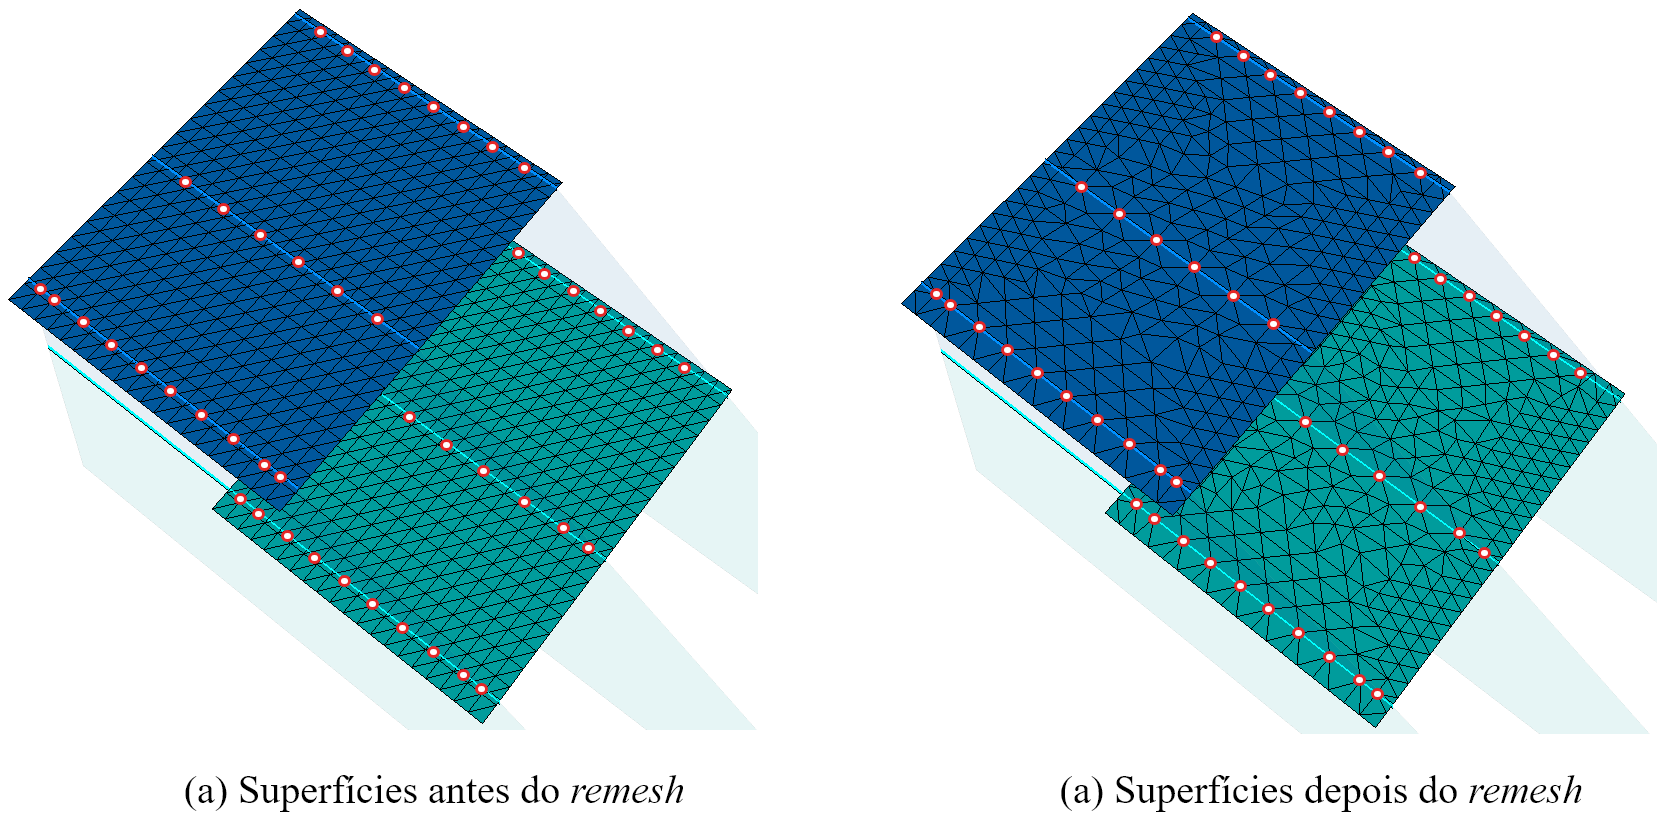
\includegraphics[width=\textwidth]{images/fig-example-1-3}
    \caption{Superfícies de horizonte antes e depois do \textit{remesh} para inclusão das \textit{LMModels} nas malhas.}\label{fig-example-1-3}
  \end{center}
\end{figure}

Logo depois do \textit{remesh}, parte-se para a definição das bordas origem e destino da superfície de horizonte do topo, que são aquelas que deverão se unir ao fim da deformação aplicada à superfície. Na Figura~\ref{fig-example-1-4} é possível notar os nós da borda dos pedaços de superfície do topo, dentre esses nós estão marcados aqueles que formam o trecho de borda de destino e origem, também sinalizados na Figura~\ref{fig-example-1-4}.

\begin{figure} [H]
  \begin{center}
    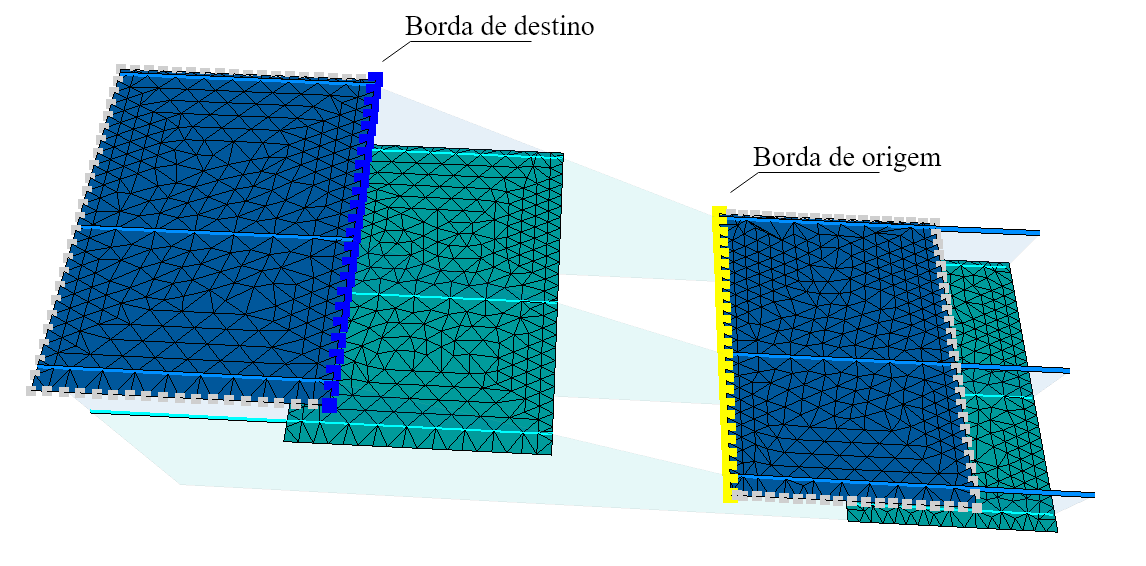
\includegraphics[width=350pt]{images/fig-example-1-4}
    \caption{Seleção das bordas de origem e destino do exemplo 1.}\label{fig-example-1-4}
  \end{center}
\end{figure}

Na etapa seguinte, calculam-se as direções dos pontos de borda e também a definição dos pontos que se movem ou não da malha da superfície. Esses dois passos são feitos após a confirmação da escolha das bordas, de forma automática. Finalmente, é chamado o algoritmo do deformador de superfícies. A próxima imagem na Figura~\ref{fig-example-1-5} mostra as superfícies deformadas segundo a restauração das seções. À direita são vistos, em destaque, os pontos da superfície que foram marcados como \quotes{move}, em verde e \quotes{não move}, em vermelho.

\begin{figure} [H]
  \begin{center}
    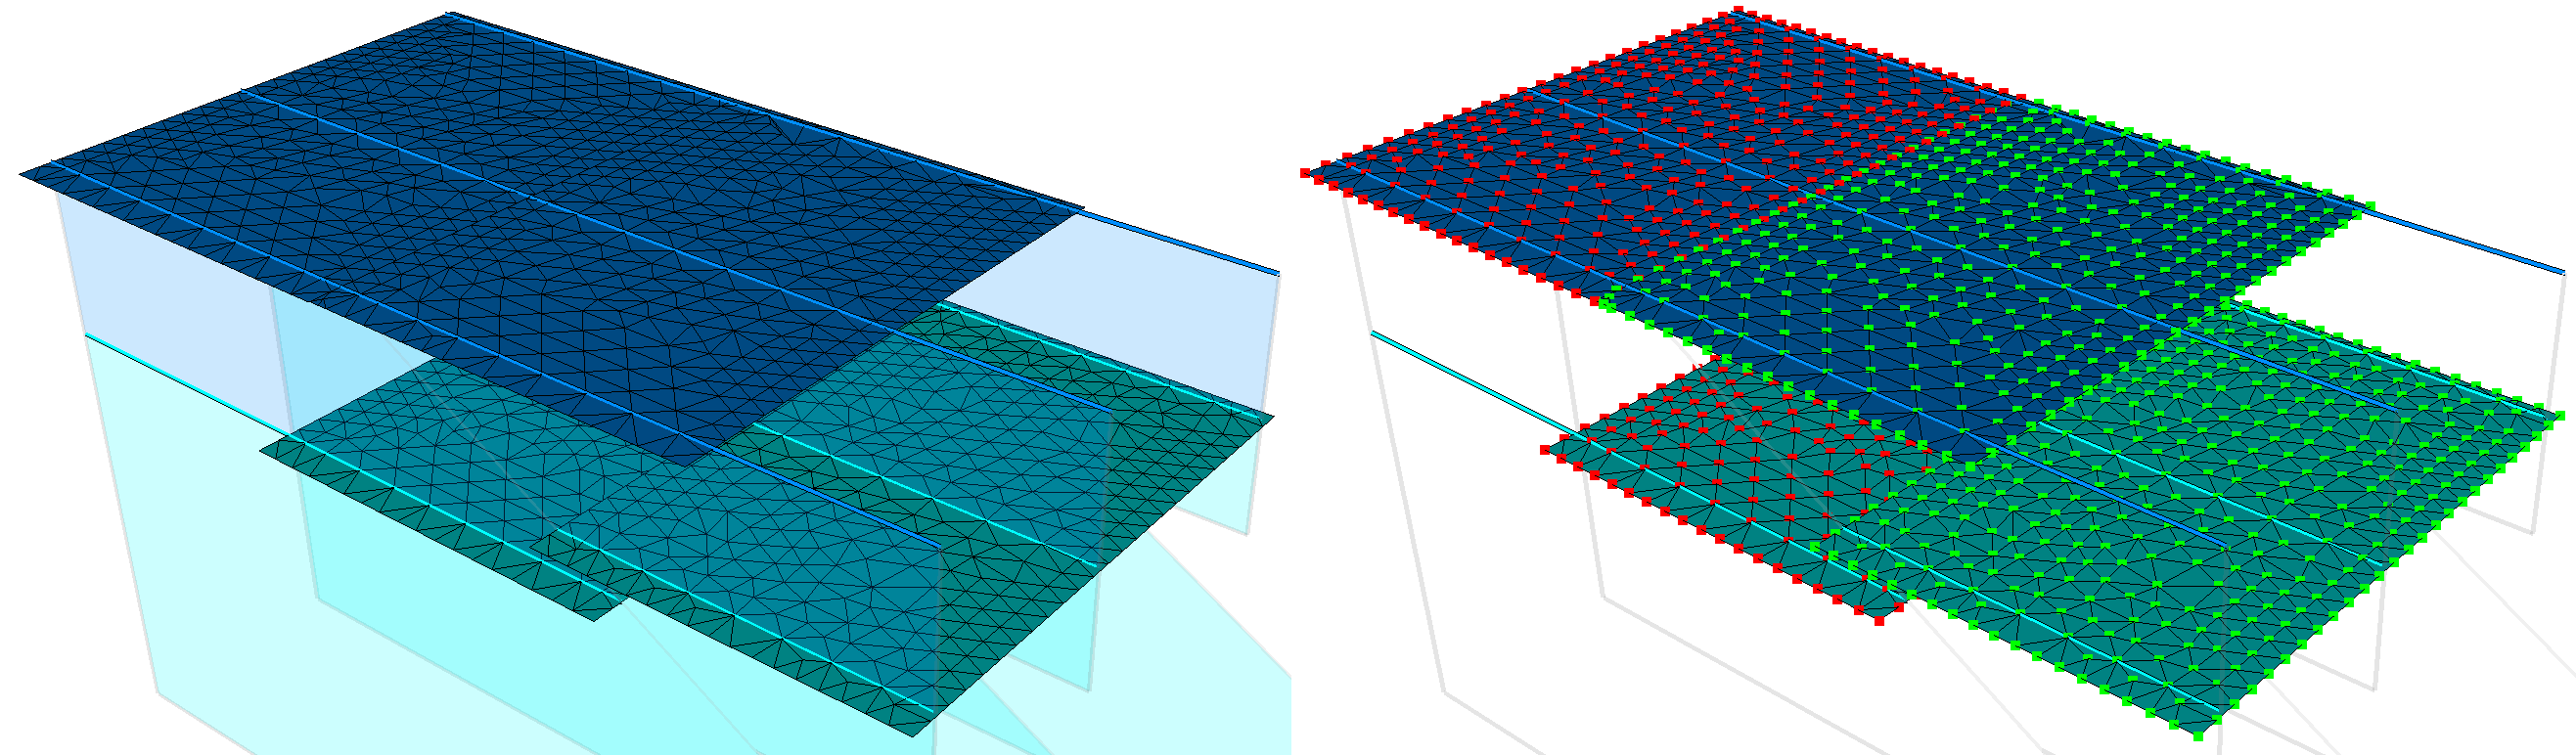
\includegraphics[width=\textwidth]{images/fig-example-1-5}
    \caption{Mapeamento de superfície do modelo de exemplo 1.}\label{fig-example-1-5}
  \end{center}
\end{figure}

O deformador de superfícies é chamado uma vez para cada superfície do modelo, no entanto, apenas a superfície do topo possui um conjunto de pontos de controle na borda próxima à falha que está sendo restaurada, ficando assim, as superfícies mais velhas sendo deformadas apenas com base na restauração das seções através das \textit{LMModels}.

\subsection{Exemplo: modelo geológico Cenpes}\label{ex-2-surf}

Este segundo exemplo utiliza um modelo geológico adaptado cedido pelo Centro de Pesquisa, Desenvolvimento e Inovação Leopoldo Américo Miguez de Mello (Cenpes/Petrobras)~\cite{Cenpes}, com dois horizontes e sete falhas com suas respectivas superfícies. No modelo foram criadas e restauradas 16 seções e conta ao todo com 14 \textit{EtapasMS}. A Figura~\ref{fig-example-2-1} mostra o modelo geológico numa vista tridimensional de cima (a) com a superfície do horizonte mais recente e (b) da superfície do horizonte mais antigo além da identificação das falhas. E a Figura~\ref{fig-example-2-2} exibe as seções geológicas numa vista tridimensional.

\begin{figure} [H]
  \begin{center}
    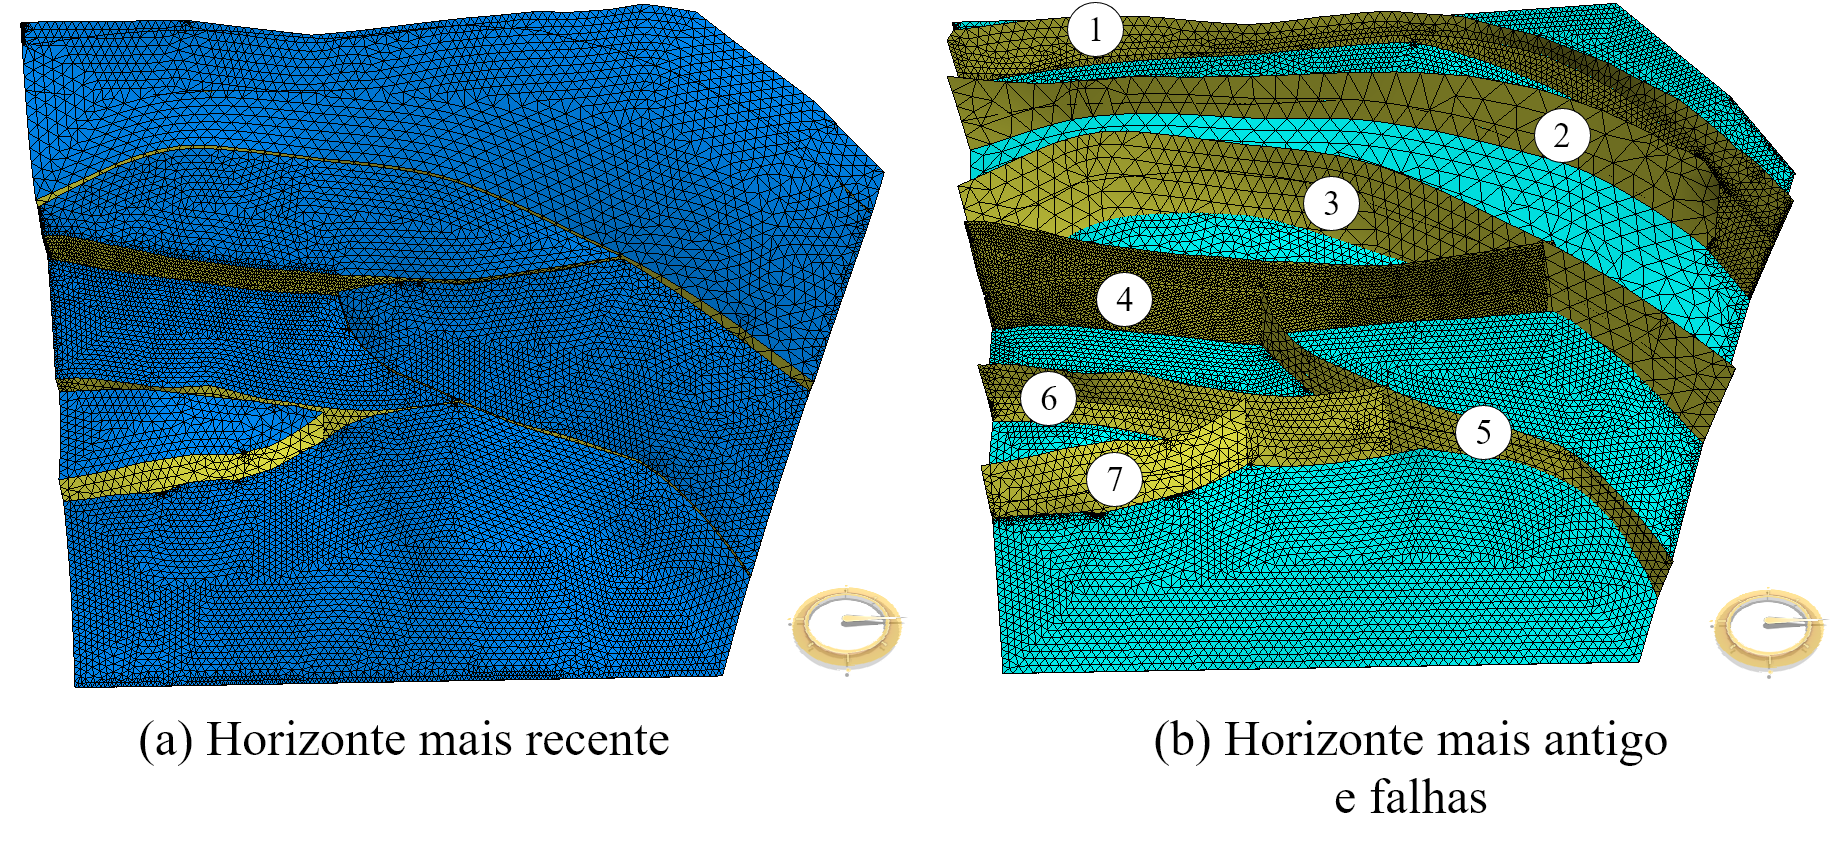
\includegraphics[width=\textwidth]{images/fig-example-2-1}
    \caption{Vista de cima do modelo geológico adaptado cedido pelo Cenpes.}\label{fig-example-2-1}
  \end{center}
\end{figure}



\begin{figure} [H]
  \begin{center}
    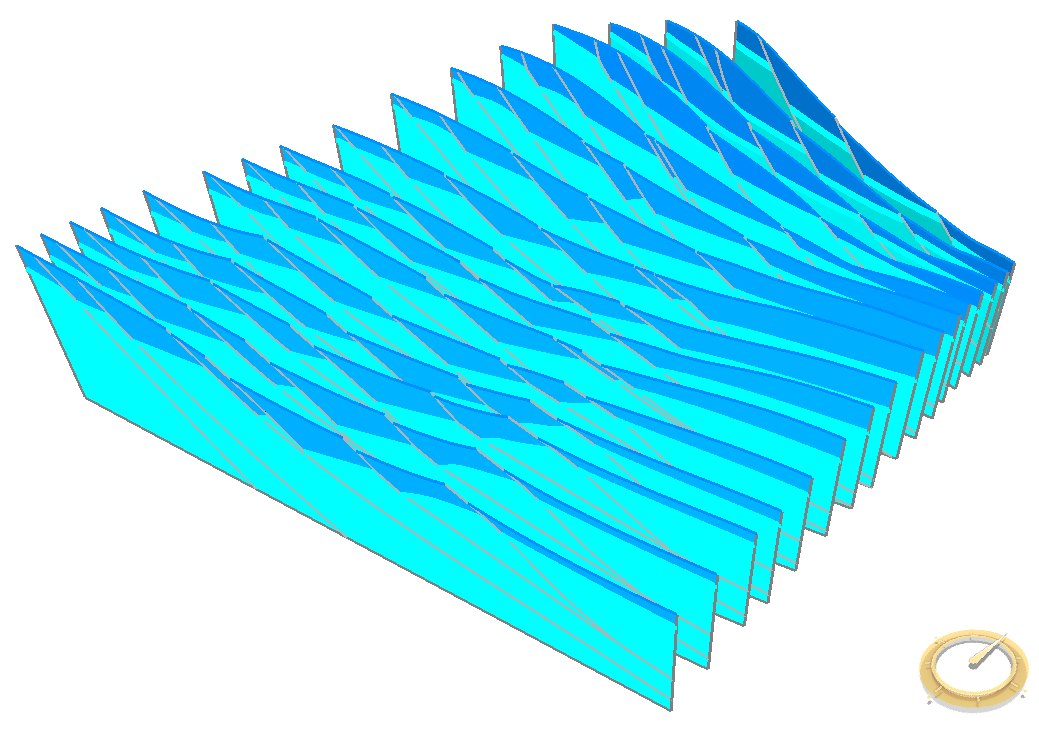
\includegraphics[width=320pt]{images/fig-example-2-2}
    \caption{Vista das seções que compõem o modelo geológico adaptado cedido pelo Cenpes.}\label{fig-example-2-2}
  \end{center}
\end{figure}

Conforme mencionado, a primeira ação para iniciar o mapeamento de superfícies é a criação das \textit{LMModels} a partir das seções geológicas restauradas e após isso criar a estrutura de dados como apresentado na Figura~\ref{fig-lmm-data-structure}. As \textit{LMModels} das seções no ambiente multisseção do Sistema Recon são apresentadas na Figura~\ref{fig-example-2-3}.

\begin{figure} [H]
  \begin{center}
    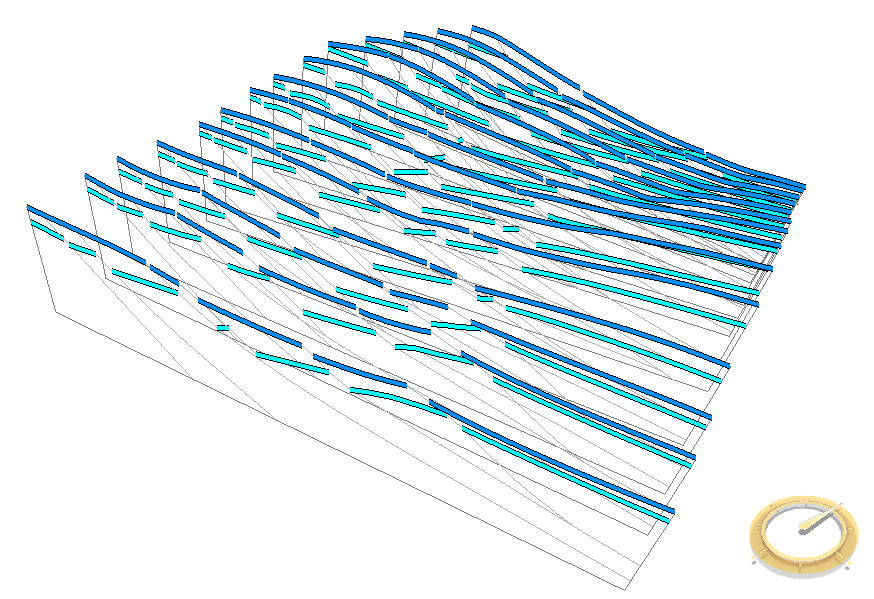
\includegraphics[width=320pt]{images/fig-lmmodel-ms}
    \caption{Vista das \textit{LMModels} do modelo geológico adaptado cedido pelo Cenpes.}.\label{fig-example-2-3}
  \end{center}
\end{figure}

Com as \textit{LMModels} criadas, parte-se então para o \textit{remesh} das malhas das superfícies para inclusão dos nós das \textit{LMModels} da primeira \textit{EtapaMS}. Conforme já visto, a regeração das malhas de superfícies com os pontos da \textit{LMModels} é importante para que haja uma ligação direta com o que ocorre nas seções e assim ter a principal base de dados vindos da seção para o mapeamento de superfícies. A nova malha da superfície do topo é mostrada na Figura~\ref{fig-example-2-4} juntamente das \textit{LMModels}.

\begin{figure} [h]
  \begin{center}
    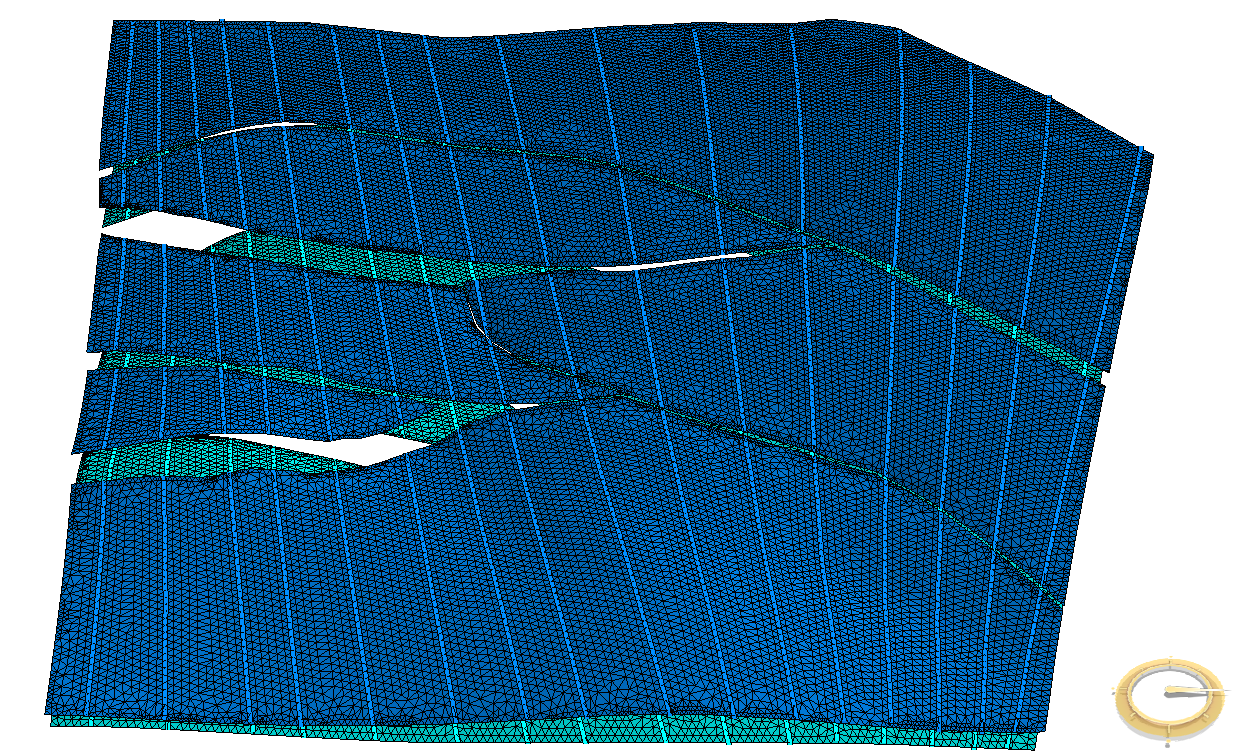
\includegraphics[width=\textwidth]{images/fig-example-2-3}
    \caption{Visão geral da nova malha de superfície do modelo geológico adaptado cedido pelo Cenpes.}\label{fig-example-2-4}
  \end{center}
\end{figure}

A primeira \textit{EtapaMS} possui os cenários das seções que restauram a falha 7, que são um total de 6 seções, como mostra a Figura~\ref{fig-example-2-5}. Nesta \textit{EtapaMS} apenas as seções que cortam a falha 7 se movimentam. Essa forma de organizar as cenários que realizam a mesma atividade em uma \textit{EtapaMS} é muito importante para o mapeamento de superfícies, pois favorece um comportamento coerente com a movimentação tectônica quando se deforma a superfície.

\begin{figure} [H]
  \begin{center}
    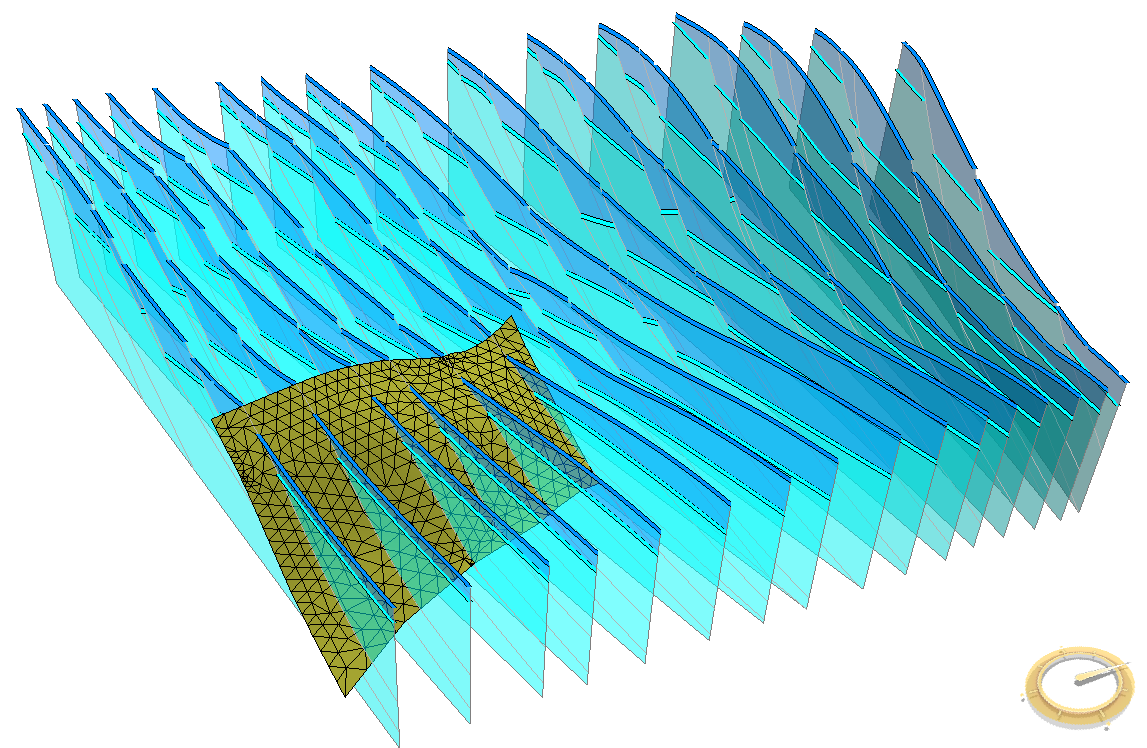
\includegraphics[width=300pt]{images/fig-example-2-5}
    \caption{Falha 7 do modelo em destaque na \textit{EtapaMS} inicial.}\label{fig-example-2-5}
  \end{center}
\end{figure}

Com a primeira falha já definida, é possível passar para a fase de seleção das bordas origem e destino na superfície do topo. São selecionados trechos de bordas de pedaços diferentes da superfície, pois a falha 7 está entre tais pedaços. As bordas origem e destino dessa primeira \textit{EtapaMS} podem ser vistas na Figura~\ref{fig-example-2-6}.

\begin{figure} [H]
  \begin{center}
    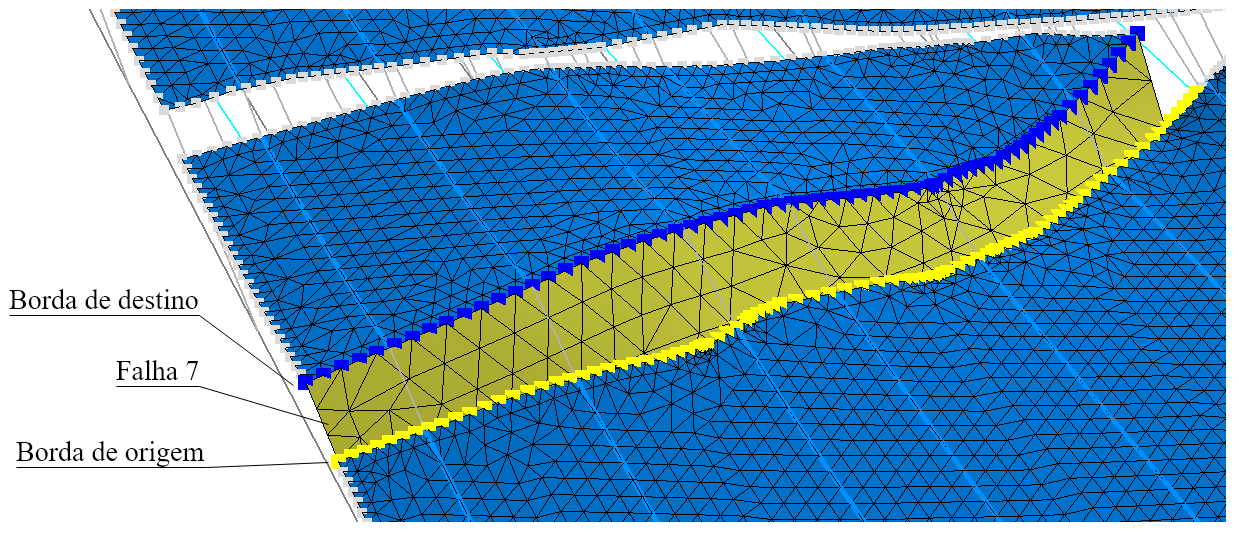
\includegraphics[width=350pt]{images/fig-example-2-6}
    \caption{Bordas origem e destino da \textit{EtapaMS} referente à falha 7.}\label{fig-example-2-6}
  \end{center}
\end{figure}

Conforme apresentado anteriormente, a fase seguinte é o cálculo dos pontos destino dos nós da borda de origem. Faz-se a definição, para cada ponto da superfície, do atributo \quotes{move} ou \quotes{não move}. Após isso pode-se executar o deformador de superfícies e o resultado (antes e depois) pode ser conferido na Figura~\ref{fig-example-2-7}.

\begin{figure} [H]
  \begin{center}
    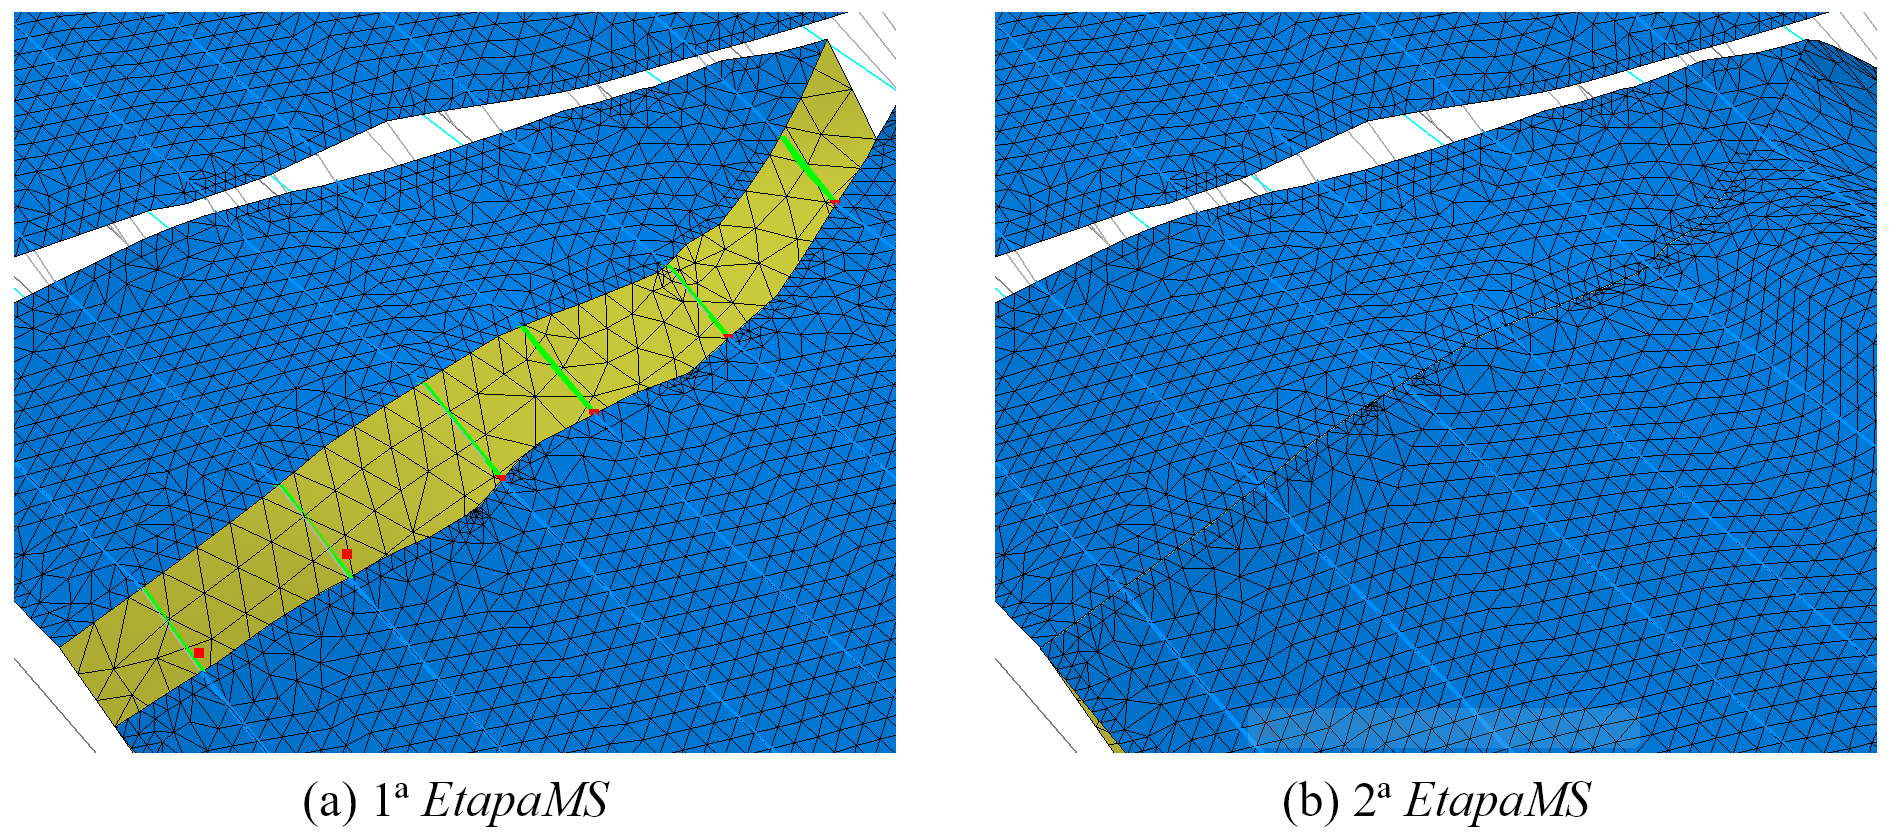
\includegraphics[width=\textwidth]{images/fig-example-2-7}
    \caption{Antes e depois da execução do deformador na superfície do topo na \textit{EtapaMS} inicial.}\label{fig-example-2-7}
  \end{center}
\end{figure}

Para a superfície mais antiga, também é chamado o deformador mas sem uma definição de bordas origem e destino, ficando restrita apenas aos pontos de controle das \textit{LMModels}. Na ilustração do antes e depois dessa superfície (Figura~\ref{fig-example-2-8}) é notável que a parte que se move não chega a coincidir com o pedaço imóvel nesta \textit{EtapaMS}, no entanto, é isso que também ocorre na restauração das seções, o que evidencia o caráter de conformidade desse mapeamento com o que acontece nas seções.

\begin{figure} [H]
  \begin{center}
    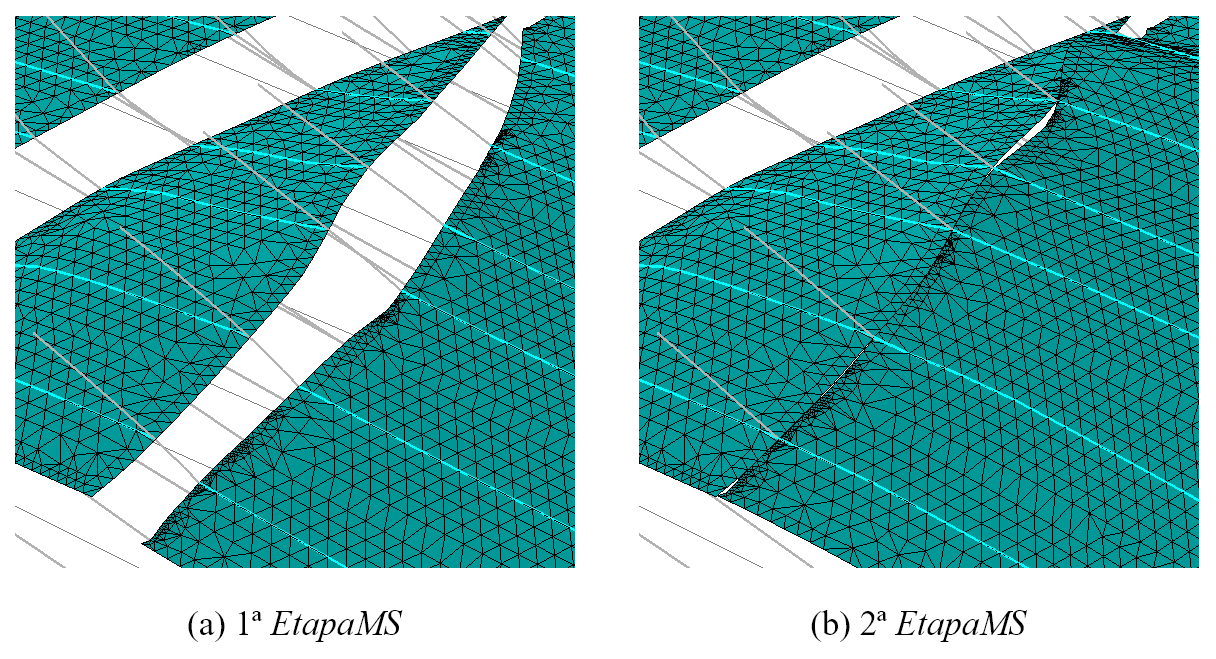
\includegraphics[width=340pt]{images/fig-example-2-8}
    \caption{Antes e depois da execução do deformador na superfície mais antiga na \textit{EtapaMS} inicial.}\label{fig-example-2-8}
  \end{center}
\end{figure}

Esse processo é repetido para cada uma das \textit{EtapasMS} do modelo, onde sempre um novo trecho de bordas origem e destino precisa ser definido (exceto em \textit{EtapaMS} de descompactação). A sequência das Figuras~\ref{fig-example-2-9} até \ref{fig-example-2-12} destaca cada um dos mapeamentos feitos com sua respectiva \textit{EtapaMS}:

\begin{figure} [H]
  \begin{center}
    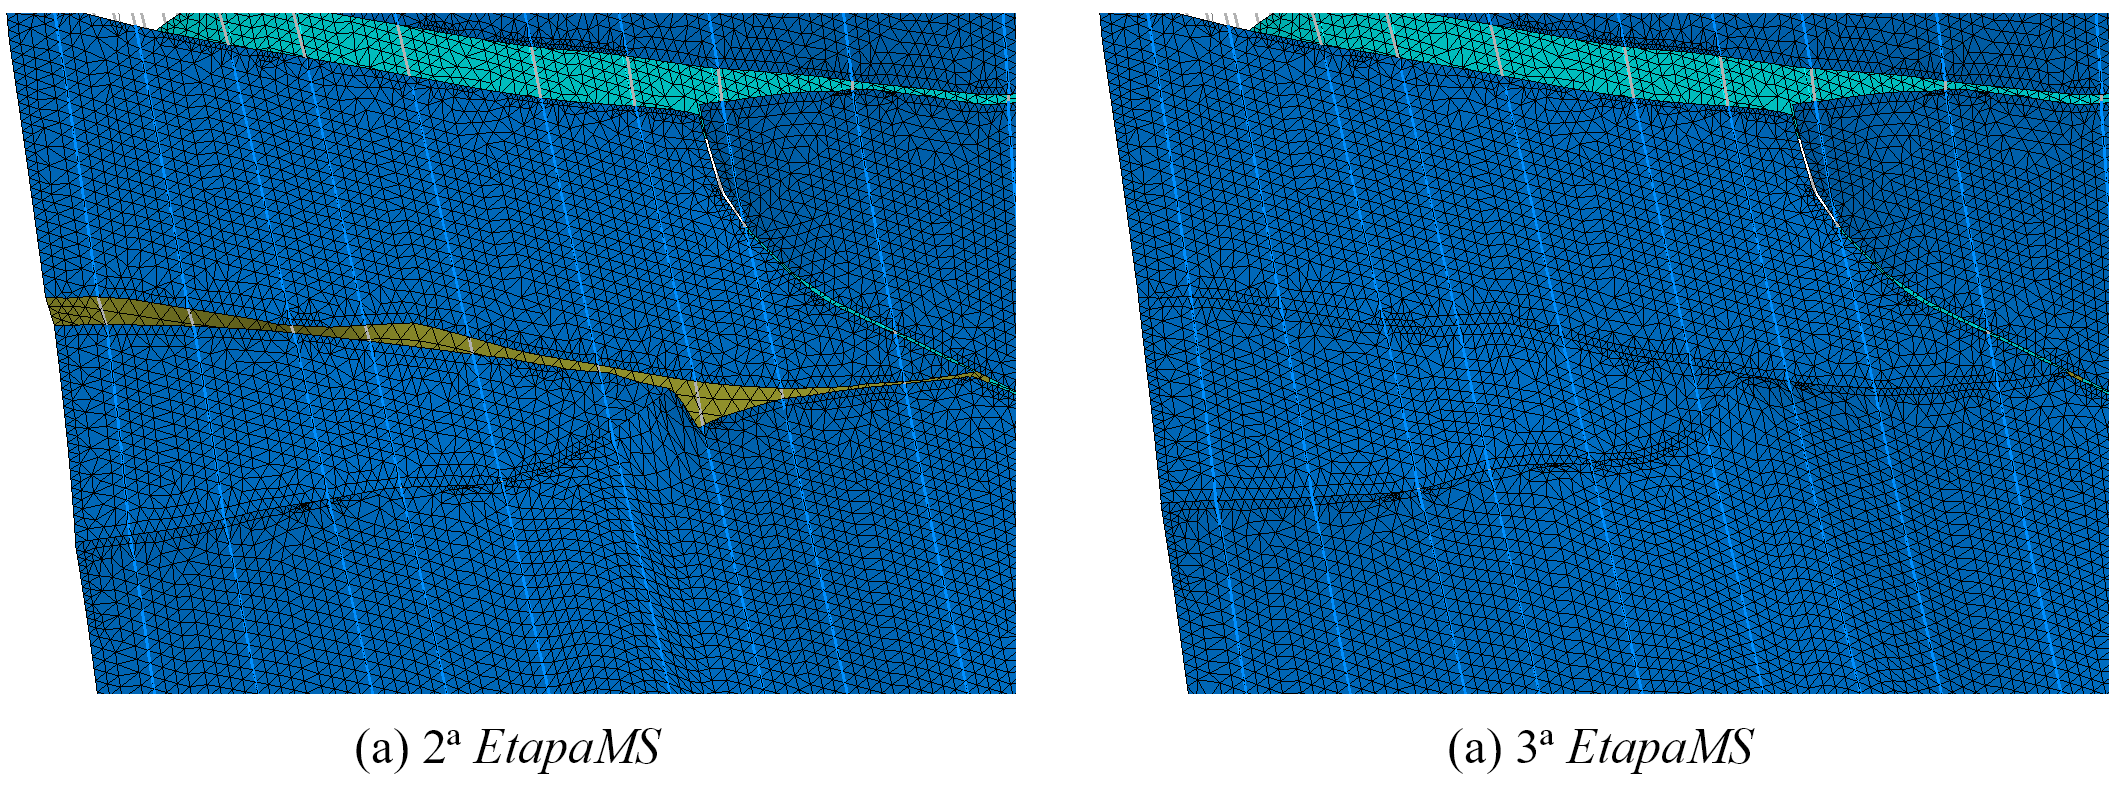
\includegraphics[width=\textwidth]{images/fig-example-2-9}
    \caption{Mapeamento da superfície conforme as seções da 2ª \textit{EtapaMS} (falha 6).}\label{fig-example-2-9}
  \end{center}
\end{figure}

\begin{figure} [H]
  \begin{center}
    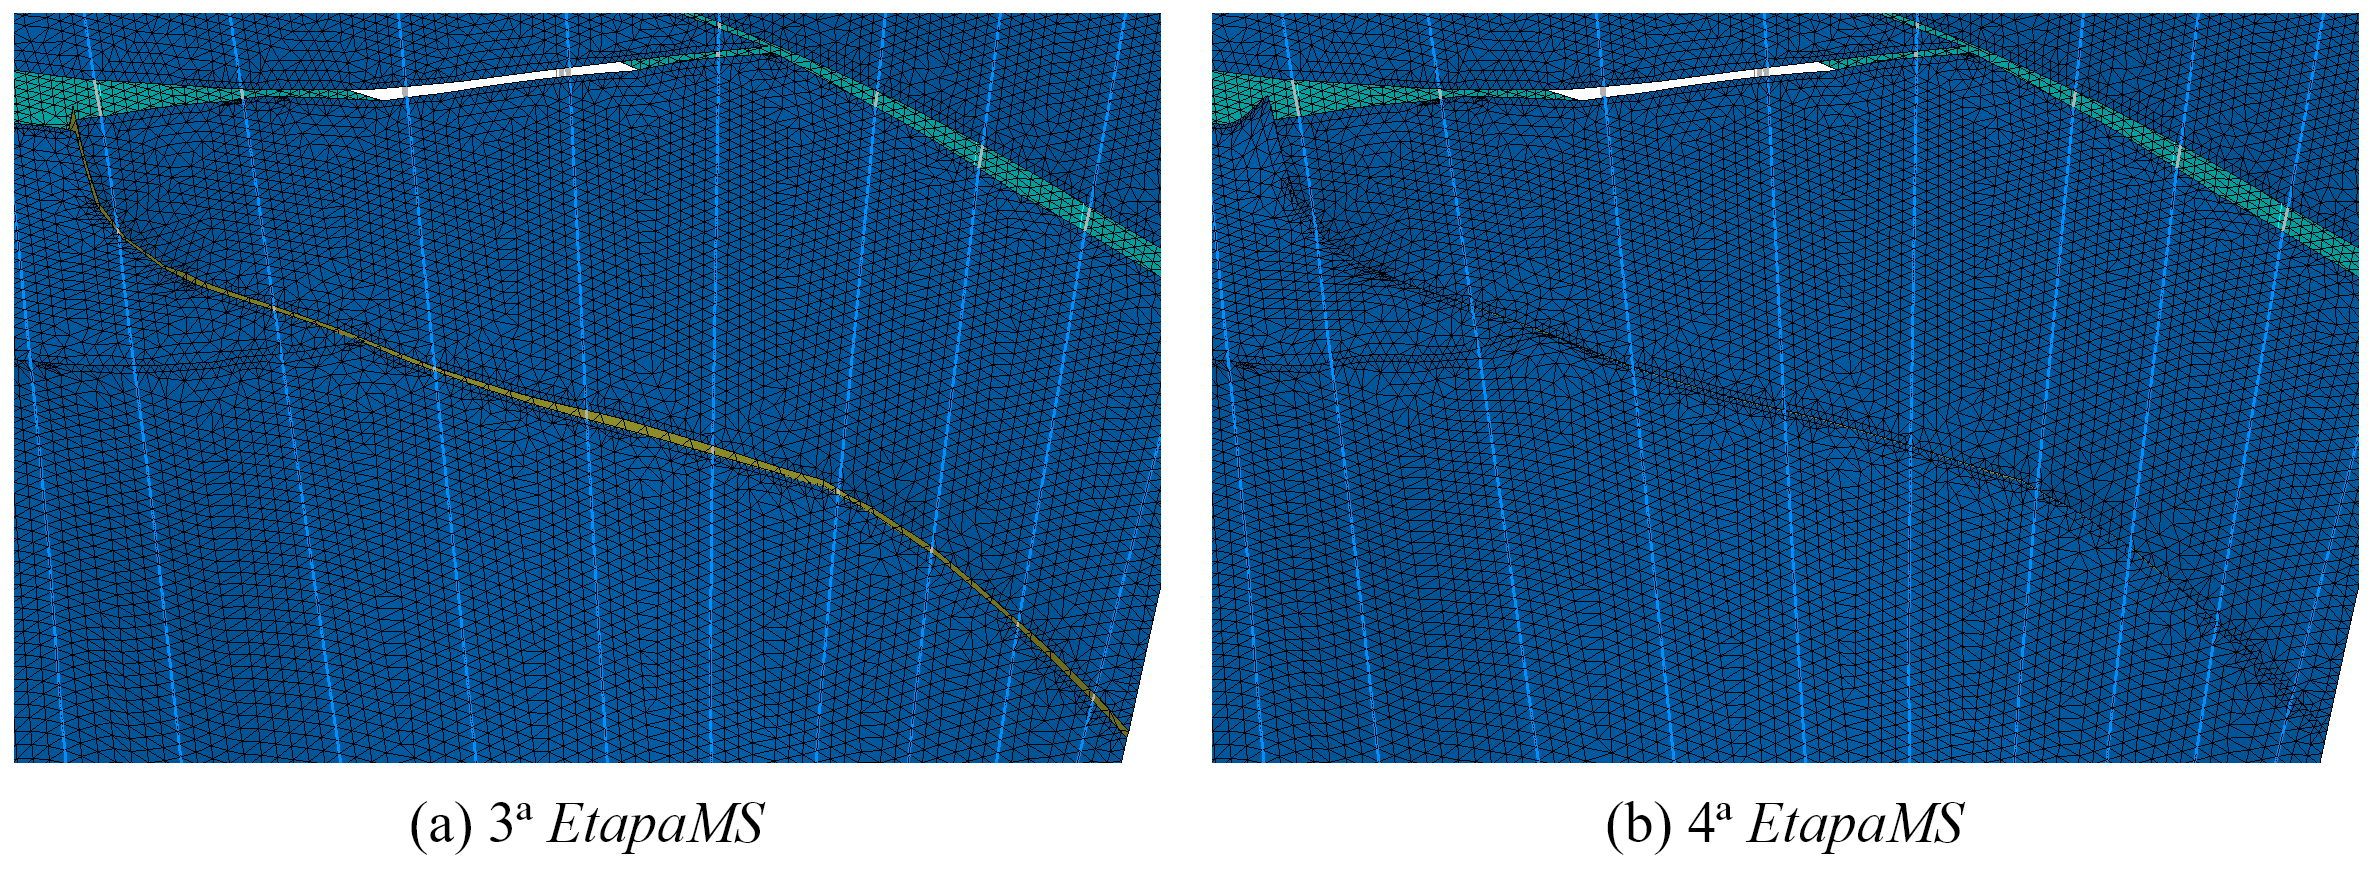
\includegraphics[width=\textwidth]{images/fig-example-2-10}
    \caption{Mapeamento da superfície conforme as seções da 3ª \textit{EtapaMS} (falha 5).}\label{fig-example-2-10}
  \end{center}
\end{figure}

\begin{figure} [H]
  \begin{center}
    \includegraphics[width=\textwidth]{images/fig-example-2-11}
    \caption{Mapeamento da superfície conforme as seções da 4ª \textit{EtapaMS} (falha 4).}\label{fig-example-2-11}
  \end{center}
\end{figure}

\begin{figure} [H]
  \begin{center}
    \includegraphics[width=\textwidth]{images/fig-example-2-12}
    \caption{Mapeamento da superfície conforme as seções da 5ª \textit{EtapaMS} (falha 3).}\label{fig-example-2-12}
  \end{center}
\end{figure}

A \textit{EtapaMS} seguinte seria com a ocorrência de uma descompactação da camada do topo, o que \quotes{alivia} a camada de baixo fazendo com que haja um soerguimento do horizonte mais antigo. Para o mapeamento, as \textit{LMModels} irão trazer essa informação e, consequentemente, todos os pontos sofrerão um deslocamento, logo, todos os nós da superfície de baixo serão marcados como \quotes{move}. Daí em diante, repete-se o processo de escolha de bordas conforme a falha da \textit{EtapaMS} corrente, com a diferença de que agora apenas a superfície de baixo existirá no modelo.

Uma última ilustração do mapeamento de superfícies nesse modelo pode ser vista na Figura~\ref{fig-example-2-13} sob um ponto de vista global.

\begin{figure} [H]
  \begin{center}
    \includegraphics[width=\textwidth]{images/fig-example-2-13}
    \caption{Mapeamento da superfície do modelo.(a) Etapa inicial, (b) falha 7, (c) falha 6, (d) falha 5, (e) falha 4 e (f) falha 5.}\label{fig-example-2-13}
  \end{center}
\end{figure}

Pela visualização do que acontece com as superfícies de horizonte se deformando a cada passo do conjunto de movimentações ocorrido nas seções, pode-se induzir que este processo, aqui chamado de mapeamento de superfícies, poderia ser nomeado de restauração de superfícies e uma breve discussão a respeito desses termos pode ser conferida no capítulo de conclusão deste trabalho.



  % -*- coding: utf-8; -*-

\chapter{Mapeamento do Volume}

No presente capítulo é apresentado o mapeamento da movimentação das seções no volume. A movimentação das seções em cada \emph{EtapaMS} de restauração acabará por determinar uma movimentação do volume. Tendo em vista que as superfícies do modelo foram mapeadas como apresentado anteriormente, a movimentação dessas superfícies também é mapeada no volume. 

Este mapeamento do volume tem o intuito de fornecer uma maneira de realizar o acompanhamento de pontos dispostos no domínio tridimensional do modelo geológico durante o processo de restauração. Com isso, é possível obter mais informações sobre o que ocorre fora das seções e superfícies geológicas.

Neste capítulo são apresentadas a metodologia para o mapeamento do volume e sua aplicação dentro do Sistema Recon, bem como detalhes sobre os requisitos para utilização do método. Uma breve discussão sobre a metodologia de mapeamento do volume também é descrita neste capítulo. A implementação computacional dessa metodologia foi realizada na biblioteca \emph{MGeo Deformer} por Müller~\cite{Muller}.

\section{Metodologia}\label{vol-metodology}

Nas últimas décadas vários métodos numéricos vêm sendo desenvolvidos para simulação de problemas físicos em modelos tridimensionais, dentre os quais destacam-se alguns, divididos em dois grupos e listados a seguir:

\renewcommand{\labelitemi}{•}
\begin{itemize}
  \item Métodos baseados em malhas tridimensionais: métodos de elementos finitos (FEM)\cite{MEF}; métodos de diferenças finitas (FDM)\cite{MDF}; métodos de volumes finitos (FVM)\cite{MVF}; métodos lagrangeanos euleriano arbitrário (ALE)\cite{ALE}.
  \item Métodos não baseados em malhas tridimensionais: método de partículas em células (PIC)\cite{PIC}; smooth particle hydrodynamics (SPH)\cite{SPH}; método de ponto material (MPM)\cite{MPM}; método de elementos discretos (DEM)\cite{DEM}; método de ponto material com interpolação generalizada (GIMP)\cite{GIMP,MullerGIMP}.
\end{itemize}

De maneira genérica, o problema físico-matemático para o mapeamento do volume baseado em restauração de seções e mapeamento de superfícies pode ser descrito por: dada a movimentação de um conjunto de seções e a movimentação de um conjunto de superfícies, movimentar um volume de forma compatível, respeitando restrições de movimentação nas falhas. Todos os métodos acima citados, além de outros não referenciados nesta lista, apresentam vantagens e desvantagens e poderiam ser utilizados para solucionar este problema. Todavia, a escolha de um método numérico deve contemplar as características do problema que por vezes demanda simplificações e/ou aprimoramentos além da avaliação da viabilidade de uso, por exemplo: tempo para simulação, geração de dados de entrada, estabilidade numérica, entre outros. De forma geral, modelos geológicos tridimensionais apresentam características de grande complexidade geométrica. Essa complexidade, por sua vez, acarreta grandes desafios para geração de malhas, especialmente quando devem ser consideradas restrições de horizontes e falhas. Além disso, de forma geral em Geologia, as etapas de modelagem e simulação tridimensionais apresentam soluções caras computacionalmente. Tendo em vista estes aspectos, Muller~\cite{Muller} desenvolveu uma metodologia de solução do problema matemático exposto anteriormente, baseada principalmente nos métodos GIMP e ALE, apresentada a seguir.

O problema físico-matemático é caracterizado pela movimentação do volume, que por sua vez é guiado pela movimentação de seções transversais e/ou superfícies. Dessa forma, as equações de conservação de massa e conservação de momento são suficientes para a solução do problema, Eqs.~\ref{eq-vol-1} e~\ref{eq-vol-2} respectivamente. Na conservação de momento, devido às características do problema, o termo relativo às forças de corpo (gravitacionais) pode ser desconsiderado.

\begin{align}
  &\frac{d\rho}{dt} + \rho \mathbf{\nabla}\cdot\boldsymbol{v} = 0\label{eq-vol-1}
\end{align}

\begin{align}
  &\rho\frac{d\boldsymbol{v}}{dt} - \mathbf{\nabla} \cdot \boldsymbol{\sigma} = 0\label{eq-vol-2}
\end{align}

Nas equações acima $\rho$ representa densidade, $\boldsymbol{v}$ velocidade e $\boldsymbol{\sigma}$ o tensor de tensões de Cauchy. Para evitar a necessidade de geração de malhas tridimensionais, a solução das Eqs.~\ref{eq-vol-1} e~\ref{eq-vol-2} será desenvolvida para um meio representado por pontos discretos arbitrários, em suas coordenadas $\boldsymbol{x}_p$, que por sua vez representam o volume $\Omega$ do modelo. A conectividade entre esses pontos será dada por uma grade volumétrica, em suas coordenadas $\boldsymbol{x}_i$.

A massa de cada ponto arbitrário pode ser descrita por:

\begin{align}
  &m_p =\int_{\Omega}\rho(\boldsymbol{x}_p)\chi(\boldsymbol{x}_p)\,d\Omega.
\end{align}

Sendo $\rho(\boldsymbol{x}_p)$ o campo de densidades e $\chi(\boldsymbol{x}_p)$ funções características. Para caracterizar a ligação entre os pontos e a grade são utilizadas funções peso $\boldsymbol{N}_{ip}$. Uma função $\boldsymbol{N}_{ip}$ representa o peso para o nó $i$ da grade avaliado na posição do ponto $p$, $\boldsymbol{N}_{ip} = \boldsymbol{N}(\boldsymbol{x}_p-\boldsymbol{x}_i)$ definido por:

\begin{align}
  &\boldsymbol{N}_{ip} = \frac{\displaystyle\int_{\Omega}\chi(\boldsymbol{x})\boldsymbol{\Phi}_i(\boldsymbol{x})\,d\Omega}{\displaystyle\int_{\Omega}\chi(\boldsymbol{x})\,d\Omega}.
\end{align}

Onde $\boldsymbol{\Phi}_i(\boldsymbol{x})$ é uma função de forma para o nó $i$. O gradiente da função peso pode ser definido por:

\begin{align}
  &\nabla\boldsymbol{N}_{ip} = \frac{\displaystyle\int_{\Omega}\chi(\boldsymbol{x})\nabla\boldsymbol{\Phi}_i(\boldsymbol{x})\,d\Omega}{\displaystyle\int_{\Omega}\chi(\boldsymbol{x})\,d\Omega}.
\end{align}

As funções características e de forma utilizadas na presente formulação são:

\begin{align}
  &\chi(\boldsymbol{x_p}) = 
    \begin{cases}
      1 &\text{se } |\boldsymbol{x_p}| < \cfrac{l}{2}\\
      0 &\text{em outro caso}
    \end{cases}\label{eq-vol-carac-1}
\end{align}

\makeatletter
\NewDocumentCommand{\eqmathbox}{o O{c} m}{%
  \IfValueTF{#1}
    {\def\eqmathbox@##1##2{\eqmakebox[#1][#2]{$##1##2$}}}
    {\def\eqmathbox@##1##2{\eqmakebox{$##1##2$}}}
  \mathpalette\eqmathbox@{#3}
}
\makeatother

\begin{align}
  &\Phi(\boldsymbol{x_p}) = 
    \begin{cases}
      \eqmathbox[eqn1]{1 - \cfrac{4\boldsymbol{x_p}^2+l}{4hl}} & \text{ se } |\boldsymbol{x_p}| < \cfrac{l}{2}\\
      \\
      \eqmathbox[eqn1]{1 - \cfrac{|\boldsymbol{x_p}|}{h}} & \text{ se } \cfrac{l}{2} \leqslant |\boldsymbol{x_p}| < h - \cfrac{l}{2}\\
      \\
      \eqmathbox[eqn1]{\cfrac{\left(h+\cfrac{l}{2}-|\boldsymbol{x_p}|\right)^2}{2hl}} & \text{ se } h-\cfrac{l}{2} \leqslant |\boldsymbol{x_p}| < h + \cfrac{l}{2}\\
      \\
      \eqmathbox[eqn1]{0} & \text{ em outro caso}
    \end{cases}\label{eq-vol-carac-2}
\end{align}

Nas Eqs.~\ref{eq-vol-carac-1} e~\ref{eq-vol-carac-2}, $h$ representa o tamanho da célula da grade e $l$ um tamanho característico definido inicialmente em função do número de pontos contidos na célula.

Como já mencionado, o volume é representado por pontos arbitrários. De forma semelhante, as seções e superfícies também serão representadas por pontos, entretanto para esses, são conhecidas suas posições iniciais e finais em cada etapa. A movimentação desses pontos, levada para os nós da grade será a responsável pela movimentação dos pontos do volume. A movimentação dos pontos de seções e superfícies pode ser convertida numa velocidade adimensional em relação ao tempo. Após isso, para um determinado tempo $t$ avalia-se em cada nó $i$ da grade a massa, momento e velocidade, respectivamente como segue:

\begin{align}
  &m_i^t = \textstyle\sum_p\boldsymbol{N}_{ip}m_p^t
\end{align}

\begin{align}
  &\boldsymbol{p}_i^t = \textstyle\sum_p\boldsymbol{N}_{ip}m_p^t\boldsymbol{v}_p^t
\end{align}

\begin{align}
  &\boldsymbol{v}_i^t = \frac{\boldsymbol{p}_i^t}{m_i^t}
\end{align}

$\sum_p$ representa a soma sobre todos os pontos que possuem contribuição para uma determinada célula da grade e $\sum_i$ representa a soma sobre todos os nós da grade que contribuem para um determinado ponto.

O passo seguinte consiste numa etapa de advecção Euleriana simples que definirá a nova posição dos pontos do volume baseada nas informações que previamente foram levadas aos nós da grade. Para isto é avaliado o gradiente da velocidade de cada ponto, o tensor gradiente de deformação de cada ponto $\boldsymbol{F}_p$, que possibilitará o cálculo de deformações no volume e a posição atualizada de cada ponto.

\begin{align}
  &\boldsymbol{v}_p^{t+\Delta t} = \textstyle\sum_i\boldsymbol{N}_{ip}\boldsymbol{v}_i^{t+\Delta t}
\end{align}

\begin{align}
  &\boldsymbol{F}_p^{t+\Delta t} = (\boldsymbol{I} + \nabla\boldsymbol{v}_p^{t+\Delta t}\Delta t) \boldsymbol{F}_p^t
\end{align}

\begin{align}
  &\boldsymbol{x}_p^{t+\Delta t} = (\boldsymbol{I} + \nabla\boldsymbol{v}_p^{t+\Delta t}\Delta t) \boldsymbol{F}_p^t
\end{align}

Os incrementos de tempo considerados para integração temporal deste problema, virtualmente transiente, consideram as condições de Courant-Friedrichs-Lewy (CFL)~\cite{CFL}, garantindo assim a estabilidade numérica da solução.

Como mencionado anteriormente, as seções e superfícies do modelo são responsáveis pela informação da movimentação que guiará a movimentação do volume. Essa movimentação, no espaço das seções e superfícies, honrou restrições de movimento dadas pelas falhas geológicas. Evidentemente, se deseja que a movimentação do volume também respeite essas restrições, ou seja, as superfícies das falhas devem ser consideradas como restrições para a movimentação do volume. Para isso, as superfícies de falha também são discretizadas por pontos. Aos pontos do volume que estarão em contato com as falhas são impostas condições especiais de movimentação. Se considerarmos em um nó $i$ da grade a velocidade de um ponto do volume $\boldsymbol{v}_i^v$ e a velocidade de um ponto da falha $\boldsymbol{v}_i^f$ teremos contato se $\left(\boldsymbol{v}_i^v-\boldsymbol{v}_i^f\right)\boldsymbol{n}_i>0$. Sendo $\boldsymbol{n}_i$ a normal da superfície da falha calculada em $i$. Se a condição de contato é satisfeita e a condição de momento garantida, as velocidade podem ser corrigidas por:

\begin{align}
  &\bar{\boldsymbol{v}}_i^v = \boldsymbol{v}^v_i - m_i^f(\boldsymbol{v}^v_i - \boldsymbol{v}^f_i)\boldsymbol{n}_i \cfrac{\boldsymbol{n}_i}{(m_i^v+m_i^f)}
\end{align}

\begin{align}
  &\bar{\boldsymbol{v}}_i^f = \boldsymbol{v}^f_i - m_i^v(\boldsymbol{v}^v_i - \boldsymbol{v}^f_i)\boldsymbol{n}_i \cfrac{\boldsymbol{n}_i}{(m_i^v+m_i^f)}
\end{align}

\iffalse
É criada um grid de células (para cálculo), cada célula tem 8 pontos.
Usa-se o GIMP, splines fruto de uma interpolação generalizada
Resolve-se a equação de momento. Tem-se as velocidades das seções e das superfícies. deslocamento/1 = velocidade.
VELOCIDADE vezes MASSA = MOMENTO

Em síntese, com 
\fi

\section{Preparação dos dados}

O uso desse procedimento dentro do Sistema Recon para realizar o mapeamento do volume requer uma série de dados extraídos da restauração das seções e do mapeamento de superfícies, nesta seção são apresentados os requisitos e o modo de tratamento dos dados.

Após isso, esse conjunto de informações é passado ao \emph{deformador de volume} que é a implementação computacional da metodologia apresentada anteriormente. O deformador de volume está presente na biblioteca \emph{MGeo Deformer}~\cite{Muller}.

Em síntese, o fluxo de trabalho para realizar o mapeamento do volume de um modelo geológico é apresentado na Figura~\ref{fig-volume-mapping-workflow} a seguir:

\begin{figure} [H]
  \begin{center}
    \includegraphics[width=\textwidth]{images/fig-volume-mapping-workflow}
    \caption{Fluxo de trabalho para executar o mapeamento do volume.}\label{fig-volume-mapping-workflow}
  \end{center}
\end{figure}

\subsection{Lista de falhas e \emph{EtapasMS}}

Assim como no mapeamento de superfícies, é preciso que o modelo esteja com a restauração das seções já finalizadas com \emph{EtapasMS} também prontas. Além disso, caso tenha sido feito o mapeamento de superfícies, é possível extrair dados desse mapeamento e assim ter ainda mais pontos contribuindo para a movimentação do volume\footnote{É possível realizar o mapeamento de superfícies em paralelo com o volume, bastando realizar a cada passo um e outro alternadamente.}.

Ao iniciar o mapeamento de volume, o primeiro passo é o levantamento de quantas \emph{EtapasMS} existem no modelo. Isso é necessário porque o mapeamento do volume também é feito por \emph{EtapaMS}, mais precisamente de uma \emph{EtapaMS} atual em relação à próxima. Ou seja, a entrada de dados vem principalmente das seções e superfícies em relação ao passo seguinte da restauração do modelo.

Após isso, busca-se todas as superfícies tridimensionais do modelo, incluindo as de falhas e horizontes. As superfícies são o principal parâmetro para a geração da nuvem de pontos que representam o volume discretizado\footnote{Para a geração da nuvem de pontos, as superfícies de horizonte precisam estar no estado original do modelo, ou seja, antes de haver deformação pelo mapeamento de superfícies. Nesse caso, são as superfícies da \emph{EtapaMS} inicial.}.

Com todos esses dados levantados, parte-se à geração da nuvem de pontos. Importante ressaltar que a geração da nuvem de pontos só é realizada uma única vez. Na etapa de descompactação serão removidos os pontos correspondentes à camada removida.

\subsection{Geração da nuvem de pontos}\label{cloud-points-generation}

A nuvem de pontos espaciais neste mapeamento, como já dito, é o volume geológico discretizado. Para sua criação, é preciso identificar o domínio tridimensional do modelo. Isto é feito com o cálculo da caixa envoltória de todo o modelo, em termos práticos, é a união das caixas envoltórias de todas as superfícies.

Com esta informação já é possível realizar a geração da grade volumétrica (Figura~\ref{fig-vol-grid}). Essa grade não é visualizada no modelo, apenas uma abstração utilizada no cálculo da movimentação e também para a geração dos pontos. Cada célula da grade é responsável por abrigar 8 pontos, como mostra a Figura~\ref{fig-vol-cell}.

\begin{figure} [H]
  \begin{center}
    \includegraphics[width=\textwidth]{images/fig-vol-grid}
    \caption{Caixa envoltória e grade volumétrica do modelo geológico.}\label{fig-vol-grid}
  \end{center}
\end{figure}

\begin{figure} [H]
  \begin{center}
    \includegraphics[width=\textwidth]{images/fig-vol-cell}
    \caption{Esquema de representação dos pontos em uma célula da grade.}\label{fig-vol-cell}
  \end{center}
\end{figure}

Cada célula possui as mesmas dimensões, na Figura~\ref{fig-vol-cell}, os comprimentos em $x$, $y$ e $z$ são obtidos pela divisão da caixa envoltória pelo número de subdivisões requerida e representados por $l_x$, $l_y$ e $l_z$ respectivamente. Os pontos internos são localizados segundo esses comprimentos; também na Figura~\ref{fig-vol-cell} as coordenadas são obtidas a partir de $a$, $b$ e $c$, que são, respectivamente, $l_x/4$, $l_z/4$ e $l_y/4$.

No entanto, apenas criar as células e então os pontos não é a única etapa. Os pontos que estão dentro da caixa envoltória mas fora do modelo geológico, precisam ser descartados. Ou seja, pontos acima da superfície de horizonte mais recente, precisam ser removidos. Além disso, dentre aqueles que restam é preciso que se defina a qual camada tal ponto pertence. Esta definição pode ser melhor explicada com uma ilustração em 2D, como na Figura~\ref{fig-vol-2d}. Cada ponto entre duas superfícies de horizonte é marcado como pertencente à camada de cima. Os pontos abaixo da última superfície (mais antiga) são definidos como pertencentes a esta.

\begin{figure} [H]
  \begin{center}
    \includegraphics[width=\textwidth]{images/fig-vol-2d}
    \caption{Esquema de representação dos pontos em uma célula da grade.}\label{fig-vol-2d}
  \end{center}
\end{figure}

Para calcular, a cada ponto, se está abaixo ou acima de uma determinada superfície, é feito uma projeção no eixo $z$ do ponto de interesse nas superfícies e a partir do resultado, são avaliadas a qual camada pertence, conforme já explicado. Nesta projeção, é feito uma busca a partir do ponto da interesse para identificar quais os elementos da superfície mais próximos a ele e então realizar a projeção. A busca é feita com o auxílio de uma estrutura de dados \emph{R-tree}~\cite{RTree} criada a partir da malha da superfície.

Apesar de todos esses recursos para se gerar os pontos, descartar os de fora do domínio e ainda marcar a qual camada ele pertence, dependendo do modelo, podem haver pontos inconsistentes ou com marcação de camada errada. Isso pode acontecer quando a superfície apresenta buracos e, portanto, naquela região não terá uma projeção em $z$ existente, com isso, o ponto recebe a marcação da superfície de baixo, incorretamente, o que faz a nuvem de pontos apresentar unidades erroneamente. Casos assim são mostrados na Figura~\ref{fig-vol-errors}.

\begin{figure} [H]
  \begin{center}
    \includegraphics[width=200pt]{images/fig-vol-errors}
    \caption{Erro passível de ocorrer na geração da nuvem de pontos.}\label{fig-vol-errors}
  \end{center}
\end{figure}

Entretanto, são casos muito isolados e tendem a se reduzir ainda mais conforme se aumente o número de células na grade volumétrica. Além do mais, são problemas que não interferem na movimentação dos pontos. É algo que deixa a nuvem de pontos menos fidedigna ao volume geológico mas nem um pouco crítico.

\subsection{Movimentação dos pontos}

Com a nuvem de pontos já criada, pode-se iniciar a movimentação desses pontos segundo o deslocamento apresentado pelas seções e superfícies entre uma \emph{EtapaMS} e outra. 

Como já dito, uma \emph{EtapaMS} é um conjunto de cenários, cada um pertencente a uma seção. Pela \emph{EtapaMS} seguinte também é possível fazer a ligação entre um cenário e outro de uma seção. Mais especificamente, pela lista de \emph{EtapasMS} pode-se ter o histórico de cenários da restauração de uma seção.

O objetivo neste passo é ter o deslocamento dos pontos das malhas da seção entre uma \emph{EtapaMS} e a próxima. Este cálculo é feito semelhantemente à interpolação das \emph{LMModels} apresentada no item~\ref{lmmodels-surface-map}. Dessa forma, para cada ponto de malha da seção na \emph{EtapaMS} $A$ vai possuir um correspondente na malha da seção na \emph{EtapaMS} $B$.

Estes pontos são colocados em uma estrutura de dados especial e cada um com um atributo armazenando o seu destino na \emph{EtapaMS} seguinte.

O mesmo é feito para as superfícies após o mapeamento delas, com a vantagem de não precisar de uma interpolação (já que a malha da superfície não muda de uma \emph{EtapaMS} a outra). Para cada ponto da malha de superfície, é registrado seu correspondente na \emph{EtapaMS} seguinte. Os pontos das superfícies são adicionados à mesma estrutura de dados dos pontos das seções.

O último dado depende do tipo de marco geológico ocorrido entre as \emph{EtapaMS}. Em caso de descompactação, só são levados em conta pontos de seções e superfícies excluindo aqueles da camada a ser removida. Já em caso de restauração de falha, é preciso pegar os nós da malha da falha que está sendo restaurada e enviar ao deformador de volume como restrição junto da estrutura de dados com os pontos das seções e superfícies. Um resumo destes passos é apresentado na Figura~\ref{fig-vol-algorithm}.

\begin{figure} [H]
  \begin{center}
    \includegraphics[width=350pt]{images/fig-vol-algorithm}
    \caption{Conjunto de dados para se fazer o mapeamento de volume.}\label{fig-vol-algorithm}
  \end{center}
\end{figure}

O resultado é uma nuvem de pontos atualizada que será usada no próximo passo do mapeamento e assim ter um volume coerente com o a movimentação tectônica das seções e superfícies.

\section{Exemplos e resultados}

Nesta seção é mostrado um exemplo de mapeamento do volume feito no mesmo modelo usado no mapeamento de superfície já apresentado no item~\ref{ex-2-surf}.

Para este exemplo foi adotada uma subdivisão para geração da grade volumétrica de $70$ unidades em $x$, $70$ unidades em $y$ e $60$ em $z$. Um total de $1.518.053$ pontos foram criados no domínio do modelo geológico\footnote{Ao realizar uma verificação simples, foram definidas $70\times70\times60=294.000$ células, cada uma contendo $8$ pontos, logo, aproximadamente $35\%$ dos pontos foram descartados por estarem fora do domínio do modelo.}. A Figura~\ref{fig-vol-ex-1} a seguir exibe o modelo geológico com apenas as superfícies de horizonte à esquerda e a nuvem de pontos gerada à direita.

\begin{figure} [H]
  \begin{center}
    \includegraphics[width=\textwidth]{images/fig-vol-ex-1}
    \caption{Superfícies do modelo geológico e nuvem de pontos gerada.}\label{fig-vol-ex-1}
  \end{center}
\end{figure}

Observa-se na imagem da direita da Figura~\ref{fig-vol-ex-1} que há pontos no topo marcados como sendo da camada geológica de baixo, isso acontece pela presença de buracos na superfície do topo, problema discutido na seção~\ref{cloud-points-generation} (Figura~\ref{fig-vol-errors}).

Neste modelo já estão feitas todas as restaurações de seções e também o mapeamento de superfície (como apresentado na seção~\ref{ex-2-surf}). A primeira \emph{EtapaMS} restaura a falha 7 do modelo. Essa falha intercepta apenas 6 seções geológicas (Figura~\ref{fig-example-2-5}), logo apenas estas seções irão contribuir com pontos, cujos deslocamentos são maiores que zero, para a movimentação do volume. 

De acordo com o apresentado anteriormente, os pontos das seções e das superfícies são unidos numa estrutura de dados onde cada ponto possui um atributo guardando sua posição final na \emph{EtapaMS} seguinte. A Figura~\ref{fig-vol-ex-2} mostra os pontos dessa estrutura para esse primeiro passo, evidenciando apenas aqueles próximo das seções cruzadas pela falha 7, além dos pontos da própria superfície de falha 7.

Conforme metodologia apresentada (seção~\ref{vol-metodology}), a movimentação conhecida dos pontos de seção e superfície é a responsável por fazer a movimentação dos pontos do volume. Para esta \emph{EtapaMS} é apresentada na Figura~\ref{fig-vol-ex-3} a nova nuvem de pontos com a execução do deformador de volume.

\begin{figure} [H]
  \begin{center}
    \includegraphics[width=\textwidth]{images/fig-vol-ex-2}
    \caption{Pontos com informação de movimentação da primeira etapa do mapeamento do volume: (a) e (c) antes do movimento, (b) e (d) após o movimento.}\label{fig-vol-ex-2}
  \end{center}
\end{figure}

\begin{figure} [H]
  \begin{center}
    \includegraphics[width=\textwidth]{images/fig-vol-ex-3}
    \caption{Movimentação da nuvem de pontos devido à primeira \emph{EtapaMS} de restauração do modelo.}\label{fig-vol-ex-3}
  \end{center}
\end{figure}

Diferente do mapeamento de superfícies, aqui no volume não há necessidade de uma interação, só é preciso que os requisitos estejam prontos (seções e superfícies). Nas Figuras~\ref{fig-vol-ex-4} a~\ref{fig-vol-ex-7} são mostrados o mapeamento do volume para cada \emph{EtapaMS} subsequente até que se tenha a camada do topo restaurada.

\begin{figure} [H]
  \begin{center}
    \includegraphics[width=\textwidth]{images/fig-vol-ex-4}
    \caption{Movimentação da nuvem de pontos devido à \emph{EtapaMS} que restaura a falha 6.}\label{fig-vol-ex-4}
  \end{center}
\end{figure}

\begin{figure} [H]
  \begin{center}
    \includegraphics[width=\textwidth]{images/fig-vol-ex-5}
    \caption{Movimentação da nuvem de pontos devido à \emph{EtapaMS} que restaura a falha 5.}\label{fig-vol-ex-5}
  \end{center}
\end{figure}

\begin{figure} [H]
  \begin{center}
    \includegraphics[width=\textwidth]{images/fig-vol-ex-6}
    \caption{Movimentação da nuvem de pontos devido à \emph{EtapaMS} que restaura a falha 4.}\label{fig-vol-ex-6}
  \end{center}
\end{figure}

\begin{figure} [H]
  \begin{center}
    \includegraphics[width=350pt]{images/fig-vol-ex-7}
    \caption{Movimentação da nuvem de pontos devido à \emph{EtapaMS} de descompactação da camada do topo.}\label{fig-vol-ex-7}
  \end{center}
\end{figure}

Quando há uma \emph{EtapaMS} de descompactação, os pontos de seções e superfícies continuam sendo guia de movimentação porém, os pontos da camada do topo são removidas da nuvem de pontos e assim manter o volume do modelo atualizado segundo o estado corrente da restauração. A Figura~\ref{fig-vol-ex-7} mostra o antes e depois da descompactação neste modelo usado como exemplo.

Conforme os resultados obtidos, a movimentação do volume pode ser vista como uma boa aproximação em relação à restauração das seções, respeitando, inclusive, a restrição das superfícies de falhas.

Este processo de mapeamento do volume apresenta facilidade de uso e representa bem modelos geológicos complexos, sem uma necessidade explícita de definição desse volume. Além do mais, o método numérico empregado é capaz de fornecer bons resultados com eficiência computacional.

Com esta metodologia tem-se a possibilidade de mapear um ponto qualquer no ambiente multisseções ao longo da restauração de um modelo geológico. Há ainda a chance de movimentar pontos de seções não restauradas com base na restauração das demais, uma forma de restaurar uma seção geológica passivamente.

  % -*- coding: utf-8; -*-

\chapter{Conclusão}

\section{Resumo}

Este trabalho propôs primeiramente uma metodologia para o mapeamento de superfícies geológicas. Uma vez atingido esse objetivo, propõe-se uma abordagem alternativa para o mapeamento volumétrico de modelos geológicos baseado em restauração de seções. Essa metodologia pode ser vista como uma estratégia visando levantar informações a respeito do comportamento de um modelo geológico tridimensional a partir da movimentação tectônica gerada pelo balanceamento de seções geológicas.

\subsection*{Sistema Recon MS}

Inicialmente foi apresentado uma breve caracterização do que se trata a restauração de seções geológicas com mais ênfase nos procedimentos que o Sistema Recon MS, base de desenvolvimento, oferece para realizar tal atividade. Dentre os recursos fornecidos, pode-se citar a estrutura de dados topológicos HED, geração de malhas em seções, transformações geométricas e as linhas de mapeamento. Para mapear as transformações geológicas sofridas pelas seções geológicas ao longo da restauração para as superfícies de horizontes, falhas e topos de sal, assim como para o volume do modelo tridimensional, são criadas nas seções as linhas de mapeamento do modelo (\emph{LMModel}). 

\subsection*{Mapeamento de superfícies}

Em relação ao mapeamento de superfícies geológicas, as seguintes atividades foram realizadas:

\renewcommand{\labelitemi}{•}
\begin{itemize}
  \item breve discussão acerca da metodologia para deformar a superfície;
  \item exportação e organização das \emph{LMModels} das seções para uso como pontos de controle na deformação das superfícies\footnote{Este item é realizado no início do mapeamento, após a restauração das seções geológicas.};
  \item recriação da malha de superfície para incluir os pontos de controle como nós da malha na etapa inicial de restauração\footnote{Esta atividade só ocorre na primeira etapa de restauração. A nova malha é mantida até o final do processo.};
  \item seleção de bordas origem e destino e cálculo da direção de movimentação de seus pontos para também serem usadas como pontos de controle;
  \item definição do conjunto de nós da malha de superfície considerados livres para se movimentar (e quais não estão) numa dada etapa de restauração;
  \item apresentação de exemplos de aplicação do mapeamento de superfícies.
\end{itemize}

\subsection*{Mapeamento do volume}

Para o mapeamento do volume, são listadas a seguir as atividades feitas:

\renewcommand{\labelitemi}{•}
\begin{itemize}
  \item apresentação da metodologia de movimentação da nuvem de pontos que representa o volume geológico;
  \item organização das \emph{EtapasMS} e levantamento das superfícies presentes no modelo;
  \item geração da nuvem de pontos na etapa inicial\footnote{A nuvem de pontos só é criada uma única vez tomando por base o estado das superfícies do modelo em seu estágio inicial.};
  \item levantamento e organização do deslocamento dos pontos da seções (e do mapeamento de superfícies) para realizar a movimentação do volume;
  \item apresentação de exemplo de uso do mapeamento de volume.
\end{itemize}

\section{Mapeamento x Restauração}

A restauração de seções geológicas é uma atividade já consagrada na interpretação estrutural e fornece resultados satisfatórios de maneira eficiente. No entanto, a consideração de apenas seções transversais de modelos geológicos, que são tridimensionais, na restauração pode acarretar na dissociação do comportamento real ocorrido. Em razão disso, pode-se partir a estudos que também levem em conta características 3D. Por outro lado, soluções tridimensionais para a restauração geológica pode ser considerado ainda hoje um problema aberto para a modelagem geológico-estrutural. Além disso, em geral tendem a ser custosos e fora do controle do geólogo no processo.

Este trabalho realizou uma busca e tratamento de informações provenientes da restauração de seções (atualmente mais entendida) e as aplicou para deformar as superfícies e movimentar uma nuvem de pontos. Esse processo foi chamado de mapeamento por tratar-se de levantamento e processamento de dados com o objetivo de caracterizar uma entidade geológica, assim como é feito no mapeamento geológico~\cite{Geoscan}. Nesse caso, o objetivo foi obter um padrão do comportamento das superfícies geológicas e do volume utilizando-se os resultados da restauração de seções.

A restauração de superfícies geológicas seria um processo análogo à restauração de seções, no entanto, com suas premissas geológicas e métodos próprios. É provável que não sejam necessárias o uso de seções transversais para esse objetivo. Mais especificamente no caso de se incluir o volume para uma restauração do modelo 3D, mais questões acerca da metodologia necessitarão ser elaboradas. 

Uma restauração 3D deve levar em conta ainda mais aspectos, como parâmetros geomecânicos além dos geométricos. Alguns autores~\cite{Santi_3dgeological, Massot, DURANDRIARD2010441} já apresentaram propostas para esta finalidade. Propostas estas que incluem uma malha volumétrica, uso de elementos finitos, caracterização do material e definição de condições de contorno entre outros aspectos.

O que foi apresentado neste trabalho foi uma proposta alternativa cujo propósito se baseou em restauração 2D para se obter uma mapeamento de informações tridimensionais a custo relativamente baixo computacionalmente.

\section{Observações}

A atividade chamada de fatiamento apresentada no item~\ref{item-section-creation} produz uma seção geológica a partir de um conjunto de superfícies tridimensionais. No entanto, a depender do estado do dado de entrada, as linhas de horizontes e falhas geradas podem não ser suficientes para que haja uma seção geológica apta para se realizar uma restauração. É comum que sejam feitas edições nas linhas como extensões e aparas a fim de fechar regiões e manter uma subdivisão planar contínua.

Estas edições acabam por gerar uma separação entre a superfície 3D e a seção bidimensional. Como as linhas de horizonte das seções são base das \emph{LMModels} usadas no mapeamento de superfícies, ao realizar a exportação dos dados para o deformador, podem ocorrer movimentações inesperadas e assim obter resultados não coerentes com a restauração de seções. Consequentemente, isto se estende à realização do mapeamento do volume.

\section{Propostas para trabalhos futuros}

Em primeiro lugar, sendo este trabalho uma maneira de utilizar informações 2D para obter resultados tridimensionais, é fundamental que sejam desenvolvidos mecanismos e ferramentas que estabeleçam e persistam conexões entre as duas estruturas do modelo (seções e superfícies). Isto garantirá uma maior consistência às informações presentes no modelo geológico.

A edição nas linhas pós-criação das seções geológicas são sempre passíveis de acontecer. Como são nas seções que todo o trabalho de restauração ocorre, o modelo geológico deve ser guiado por estas alterações feitas pelos geólogos. Em outros termos, edições nas linhas das seções devem ser propagadas às superfícies para manter a coesão entre essas partes, uma vez que representam a mesma entidade geológica sob pontos de vista diferentes.

Pode-se concluir que tanto para a restauração 3D baseada em seções transversais quanto em uma restauração 3D propriamente dita, é fundamental que os dados de entrada das superfícies geológicas iniciais para o processo de restauração tenham consistência geométrica. Esse pré-requisito justifica a necessidade de se desenvolver uma ferramenta adicional para compatibilizar geometricamente as superfícies de entrada, uma vez que essas superfícies iniciais, em quase toda a totalidade dos casos, apresentam inconsistências geométricas. Esta é uma importante proposta para trabalho futuro.

Em relação ao mapeamento do volume, como já citado, é dada a possibilidade de manter um acompanhamento de um ponto qualquer no domínio do modelo geológico ao longo de cada passo da restauração. Pode-se inclusive trabalhar na movimentação de uma seção geológica inteira a partir da restauração de seções vizinhas. Propõe-se ainda uma aplicação das transformações geológicas, que são usadas nas seções, no volume como uma maneira de movimentar a nuvem de pontos sem depender somente dos pontos das seções.

Para o mapeamento tridimensional (superfícies e volume) de maneira geral, deve-se atentar para uma aperfeiçoamento na metodologia adotada na definição da direção das seções geológicas. É provável que seja necessário o uso de seções com aspecto mais restrito quanto à presença de muitas falhas. Em outras palavras, seções mais locais, definidas individualmente na região de um rejeito de falha. É possível afirmar que seções geológicas corretamente definidas tendem a tornar o processo de mapeamento mais próximo ainda de uma restauração de superfícies e volume.

Um último trabalho sugerido é o desenvolvimento de uma solução 3D com controle do usuário para a restauração tridimensional. Neste caso, um trabalho baseado nas metodologias de deformação de superfícies e volume apresentadas nesta dissertação, porém, sem a necessidade de definir seções geológicas mas sim um manuseio direto no modelo 3D.
  \arial
  \bibliography{tiny}
  \normalfont
  %% -*- coding: utf-8; -*-

\appendix
\chapter{Published paper}

The following paper was published ...

\end{document}
